\documentclass[11pt]{article}
\usepackage[a4paper,margin=2.2cm]{geometry}
\usepackage[numbers]{natbib}
\usepackage{amsmath,amssymb,booktabs,graphicx,siunitx}
\usepackage{xr}
\externaldocument{main}
\renewcommand{\thesection}{S\arabic{section}}
\renewcommand{\thetable}{S\arabic{table}}
\renewcommand{\thefigure}{S\arabic{figure}}
\renewcommand{\theequation}{S\arabic{equation}}
% Generated by scripts/jpc_v6_numbers.py -- do not edit.
\newcommand{\vZNnone}{91.11}  % antiwindup_ablation
\newcommand{\vZNbc}{0.97}  % antiwindup_ablation
\newcommand{\vZNbccv}{0.88}  % antiwindup_ablation
\newcommand{\vZNsign}{104.12}  % antiwindup_ablation
\newcommand{\vZNamp}{22.10}  % antiwindup_ablation
\newcommand{\vZNrateunc}{0.93}  % antiwindup_ablation
\newcommand{\vZNdir}{0.94}  % antiwindup_ablation
\newcommand{\vZNsignMp}{842.5}  % antiwindup_ablation
\newcommand{\vZNatmax}{3.86}  % antiwindup_mechanism
\newcommand{\vZNdiscrep}{4474}  % antiwindup_mechanism
\newcommand{\vCCnone}{87.37}  % antiwindup_ablation
\newcommand{\vCCbc}{0.87}  % antiwindup_ablation
\newcommand{\vCCbccv}{0.82}  % antiwindup_ablation
\newcommand{\vCCsign}{102.67}  % antiwindup_ablation
\newcommand{\vCCamp}{20.60}  % antiwindup_ablation
\newcommand{\vCCrateunc}{1.10}  % antiwindup_ablation
\newcommand{\vCCdir}{1.02}  % antiwindup_ablation
\newcommand{\vCCsignMp}{842.5}  % antiwindup_ablation
\newcommand{\vCCatmax}{4.06}  % antiwindup_mechanism
\newcommand{\vCCdiscrep}{3540}  % antiwindup_mechanism
\newcommand{\vlatcherr}{-16.72}  % antiwindup_mechanism
\newcommand{\vlatchgap}{16.72}  % antiwindup_mechanism (|T(t_f) - T_sp|)
\newcommand{\vlatchTmin}{377.8}  % antiwindup_mechanism
\newcommand{\vZNnominal}{0.940}  % benchmark_table
\newcommand{\vscenampmin}{13.62}  % antiwindup_scenarios
\newcommand{\vscenampmax}{31.17}  % antiwindup_scenarios
\newcommand{\vscendirmin}{2.87}  % antiwindup_scenarios
\newcommand{\vscendirmax}{4.39}  % antiwindup_scenarios
\newcommand{\vZNfivesign}{205.97}  % antiwindup_scenarios
\newcommand{\vZNfivenone}{81.26}  % antiwindup_scenarios
\newcommand{\vCCfivesign}{224.77}  % antiwindup_scenarios
\newcommand{\vCCfivenone}{78.56}  % antiwindup_scenarios
\newcommand{\vZNloadsign}{77.21}  % antiwindup_scenarios
\newcommand{\vZNloadnone}{26.65}  % antiwindup_scenarios
\newcommand{\vCCloadsign}{72.02}  % antiwindup_scenarios
\newcommand{\vCCloadnone}{26.14}  % antiwindup_scenarios
\newcommand{\vsbZNlowtime}{5.38}  % smax_signblind_diagnostics
\newcommand{\vsbZNlowerr}{+54.2}  % smax_signblind_diagnostics
\newcommand{\vsbZNlowrate}{0.72}  % smax_signblind_diagnostics
\newcommand{\vTinf}{377.94}  % CSTRPlant.find_steady_state(q_j=300)
\newcommand{\vZNIstar}{945}  % u_max - u_bias + |Kp|(T_sp - T_inf); Kp from benchmark_table
\newcommand{\vCCIstar}{1050}  % u_max - u_bias + |Kp|(T_sp - T_inf); Kp from benchmark_table
\newcommand{\vZNtkzero}{6.16}  % latch_check
\newcommand{\vZNIkzero}{4506}  % latch_check
\newcommand{\vZNDbar}{1754}  % latch_check (D bound from Eq. 10 and the band)
\newcommand{\vZNdelta}{0.13}  % latch_check
\newcommand{\vZNlatchmargin}{1801}  % latch_check
\newcommand{\vCCtkzero}{5.96}  % latch_check
\newcommand{\vCCIkzero}{3546}  % latch_check
\newcommand{\vCCDbar}{1419}  % latch_check (D bound from Eq. 10 and the band)
\newcommand{\vCCdelta}{0.13}  % latch_check
\newcommand{\vCClatchmargin}{1070}  % latch_check
\newcommand{\vttmmmax}{1.02}  % antiwindup_tt_summary
\newcommand{\vttmmmin}{0.90}  % antiwindup_tt_summary
\newcommand{\vttmmmaxpct}{2}  % antiwindup_tt_summary
\newcommand{\vttmmminpct}{10}  % antiwindup_tt_summary
\newcommand{\vttsqrtmax}{1.37}  % antiwindup_tt_summary
\newcommand{\vttsqrtmin}{0.98}  % antiwindup_tt_summary
\newcommand{\vttsqrtmaxpct}{37}  % antiwindup_tt_summary
\newcommand{\vttsqrtminpct}{2}  % antiwindup_tt_summary
\newcommand{\vtttimax}{1.97}  % antiwindup_tt_summary
\newcommand{\vtttimin}{0.90}  % antiwindup_tt_summary
\newcommand{\vtttimaxpct}{97}  % antiwindup_tt_summary
\newcommand{\vtttiminpct}{10}  % antiwindup_tt_summary
\newcommand{\vttcvmax}{1.02}  % antiwindup_tt_summary
\newcommand{\vttcvmin}{0.86}  % antiwindup_tt_summary
\newcommand{\vttcvmaxpct}{2}  % antiwindup_tt_summary
\newcommand{\vttcvminpct}{14}  % antiwindup_tt_summary
\newcommand{\vttoutside}{ZN, CC and SIMC}  % antiwindup_tt_summary (unrestricted T_t^sel outside [T_d, T_i])
\newcommand{\vttfreemaxgain}{0.00}  % antiwindup_tt_summary (largest drop of the +-5 K worst ratio when leaving the range)
\newcommand{\vttfreemaxloss}{0.08}  % antiwindup_tt_summary (largest rise of the +-5 K worst ratio when leaving the range)
\newcommand{\vttcvlower}{ZN and CC}  % antiwindup_tt_summary (T_t^sel = T_d)
\newcommand{\vttcvupper}{SIMC}  % antiwindup_tt_summary (T_t^sel = T_i)
\newcommand{\vttfreeZN}{0.020}  % antiwindup_tt_summary
\newcommand{\vttfreeCC}{0.020}  % antiwindup_tt_summary
\newcommand{\vttfreexZN}{0.009}  % antiwindup_tt_summary (free choice, exact factor)
\newcommand{\vttfreexCC}{0.008}  % antiwindup_tt_summary (free choice, exact factor)
\newcommand{\vttfreediffmax}{0.08}  % antiwindup_tt_summary (largest |free - cv| of the +-5 K worst ratio)
\newcommand{\vttfreediffloop}{SIMC}  % antiwindup_tt_summary
\newcommand{\vttfreediffrest}{0.01}  % antiwindup_tt_summary (other loops)
\newcommand{\vttfreexgain}{0.01}  % antiwindup_tt_summary (largest drop of the +-5 K worst ratio, exact free choice vs T_t^sel)
\newcommand{\vttfreeSIMCovTi}{10}  % antiwindup_tt_summary (free T_t^sel / T_i)
\newcommand{\vSIMCcvtwo}{1.15}  % antiwindup_tt_sweep
\newcommand{\vSIMCtitwo}{1.15}  % antiwindup_tt_sweep
\newcommand{\vSIMCcvm}{3.80}  % antiwindup_tt_sweep
\newcommand{\vSIMCtim}{3.80}  % antiwindup_tt_sweep
\newcommand{\vSIMCcvp}{3.17}  % antiwindup_tt_sweep
\newcommand{\vSIMCtip}{3.17}  % antiwindup_tt_sweep
\newcommand{\vempTVlower}{5}  % antiwindup_tt_tvmp (ZN and CC cases with lower TV under BC)
\newcommand{\vempMplower}{5}  % antiwindup_tt_tvmp (ZN and CC cases with lower overshoot under BC)
\newcommand{\vempcases}{6}  % antiwindup_tt_tvmp
\newcommand{\vCCfiveTVdir}{241.9}  % antiwindup_tt_tvmp
\newcommand{\vCCfiveTVbc}{101.2}  % antiwindup_tt_tvmp
\newcommand{\vCCfiveMpdir}{40.8}  % antiwindup_tt_tvmp
\newcommand{\vCCfiveMpbc}{11.3}  % antiwindup_tt_tvmp
\newcommand{\vrestcases}{9}  % antiwindup_tt_tvmp (TL, SIMC, Optimal ITAE)
\newcommand{\vrestTVhigher}{6}  % antiwindup_tt_tvmp (TL, SIMC, Optimal ITAE cases with higher TV under BC)
\newcommand{\vrestMphigher}{6}  % antiwindup_tt_tvmp (TL, SIMC, Optimal ITAE cases with higher overshoot under BC)
\newcommand{\vSIMCfiveTVdir}{30.7}  % antiwindup_tt_tvmp
\newcommand{\vSIMCfiveTVbc}{42.5}  % antiwindup_tt_tvmp
\newcommand{\vOPTfiveMpdir}{8.7}  % antiwindup_tt_tvmp
\newcommand{\vOPTfiveMpbc}{12.5}  % antiwindup_tt_tvmp
\newcommand{\vTLfiveMpdir}{11.1}  % antiwindup_tt_tvmp
\newcommand{\vTLfiveMpbc}{13.0}  % antiwindup_tt_tvmp
\newcommand{\vSIMCtvincmin}{20}  % antiwindup_tt_tvmp
\newcommand{\vSIMCtvincmax}{38}  % antiwindup_tt_tvmp
\newcommand{\vmapZNmin}{7.9}  % smax_regime_map
\newcommand{\vmapZNmax}{38.3}  % smax_regime_map
\newcommand{\vmapZNtwenty}{7.9}  % smax_regime_map
\newcommand{\vmapZNeighty}{23.5}  % smax_regime_map
\newcommand{\vmapZNlast}{36.3}  % smax_regime_map
\newcommand{\vmapCCmin}{7.4}  % smax_regime_map
\newcommand{\vmapCCmax}{37.7}  % smax_regime_map
\newcommand{\vmapCCtwenty}{7.4}  % smax_regime_map
\newcommand{\vmapCCeighty}{20.3}  % smax_regime_map
\newcommand{\vmapCClast}{37.7}  % smax_regime_map
\newcommand{\vmapTLmin}{1.2}  % smax_regime_map
\newcommand{\vmapTLmax}{2.1}  % smax_regime_map
\newcommand{\vmapTLtwenty}{2.1}  % smax_regime_map
\newcommand{\vmapTLeighty}{1.4}  % smax_regime_map
\newcommand{\vmapTLlast}{1.2}  % smax_regime_map
\newcommand{\vmapAMIGOmin}{1.1}  % smax_regime_map
\newcommand{\vmapAMIGOmax}{14.7}  % smax_regime_map
\newcommand{\vmapAMIGOtwenty}{11.5}  % smax_regime_map
\newcommand{\vmapAMIGOeighty}{1.7}  % smax_regime_map
\newcommand{\vmapAMIGOlast}{1.1}  % smax_regime_map
\newcommand{\vmapSIMCmin}{0.8}  % smax_regime_map
\newcommand{\vmapSIMCmax}{1.0}  % smax_regime_map
\newcommand{\vmapSIMCtwenty}{1.0}  % smax_regime_map
\newcommand{\vmapSIMCeighty}{0.8}  % smax_regime_map
\newcommand{\vmapSIMClast}{0.9}  % smax_regime_map
\newcommand{\vmapOptimalITAEmin}{1.3}  % smax_regime_map
\newcommand{\vmapOptimalITAEmax}{9.6}  % smax_regime_map
\newcommand{\vmapOptimalITAEtwenty}{9.3}  % smax_regime_map
\newcommand{\vmapOptimalITAEeighty}{1.8}  % smax_regime_map
\newcommand{\vmapOptimalITAElast}{1.3}  % smax_regime_map
\newcommand{\vlatchfromZN}{60}  % smax_regime_map (final error -16.7 K)
\newcommand{\vlatchfromCC}{60}  % smax_regime_map (final error -16.7 K)
\newcommand{\vretunedfirst}{11.3}  % smax_retuned
\newcommand{\vretunedlast}{1.3}  % smax_retuned
\newcommand{\vdbAMIGOdirthree}{1.22}  % antiwindup_deadband
\newcommand{\vdbZNsignthree}{105.66}  % antiwindup_deadband
\newcommand{\vdbZNampthree}{23.44}  % antiwindup_deadband
\newcommand{\vdbZNdirthree}{1.28}  % antiwindup_deadband
\newcommand{\vdbCCsignthree}{102.78}  % antiwindup_deadband
\newcommand{\vdbCCampthree}{22.12}  % antiwindup_deadband
\newcommand{\vdbCCdirthree}{1.36}  % antiwindup_deadband
\newcommand{\vdbAMIGOdirsix}{1.54}  % antiwindup_deadband
\newcommand{\vdbZNsignsix}{106.99}  % antiwindup_deadband
\newcommand{\vdbZNampsix}{24.82}  % antiwindup_deadband
\newcommand{\vdbZNdirsix}{1.65}  % antiwindup_deadband
\newcommand{\vdbCCsignsix}{104.69}  % antiwindup_deadband
\newcommand{\vdbCCampsix}{23.01}  % antiwindup_deadband
\newcommand{\vdbCCdirsix}{1.76}  % antiwindup_deadband
\newcommand{\vdbsixworstpct}{10}  % antiwindup_deadband
\newcommand{\vdbampratiomin}{13}  % antiwindup_deadband (amp-only / rate, ZN and CC)
\newcommand{\vdbsixworstpctcv}{19}  % antiwindup_deadband (rate rule vs BC T_t^sel)
\newcommand{\vopZNnone}{55.58}  % antiwindup_second_op
\newcommand{\vopZNsign}{61.48}  % antiwindup_second_op
\newcommand{\vopZNamp}{16.13}  % antiwindup_second_op
\newcommand{\vopZNdir}{1.00}  % antiwindup_second_op
\newcommand{\vopCCnone}{54.19}  % antiwindup_second_op
\newcommand{\vopCCsign}{59.68}  % antiwindup_second_op
\newcommand{\vopCCamp}{15.42}  % antiwindup_second_op
\newcommand{\vopCCdir}{1.05}  % antiwindup_second_op
\newcommand{\vopAMIGOnone}{2.16}  % antiwindup_second_op
\newcommand{\vopAMIGOsign}{2.16}  % antiwindup_second_op
\newcommand{\vopAMIGOamp}{2.16}  % antiwindup_second_op
\newcommand{\vopAMIGOdir}{1.07}  % antiwindup_second_op
\newcommand{\vopSIMCnone}{1.16}  % antiwindup_second_op
\newcommand{\vopSIMCsign}{1.16}  % antiwindup_second_op
\newcommand{\vopSIMCamp}{1.16}  % antiwindup_second_op
\newcommand{\vopSIMCdir}{1.42}  % antiwindup_second_op
\newcommand{\vSlinZN}{1.57}  % exact_robustness_table
\newcommand{\vCSZN}{490}  % exact_robustness_table
\newcommand{\vMsFZN}{4.14}  % benchmark_table
\newcommand{\vSlinCC}{1.75}  % exact_robustness_table
\newcommand{\vCSCC}{559}  % exact_robustness_table
\newcommand{\vMsFCC}{4.54}  % benchmark_table
\newcommand{\vSlinTL}{1.15}  % exact_robustness_table
\newcommand{\vCSTL}{309}  % exact_robustness_table
\newcommand{\vMsFTL}{2.32}  % benchmark_table
\newcommand{\vSlinAMIGO}{1.26}  % exact_robustness_table
\newcommand{\vCSAMIGO}{196}  % exact_robustness_table
\newcommand{\vMsFAMIGO}{1.45}  % benchmark_table
\newcommand{\vSlinSIMC}{1.11}  % exact_robustness_table
\newcommand{\vCSSIMC}{77}  % exact_robustness_table
\newcommand{\vMsFSIMC}{1.13}  % benchmark_table
\newcommand{\vSlinOptimalITAE}{1.31}  % exact_robustness_table
\newcommand{\vCSOptimalITAE}{259}  % exact_robustness_table
\newcommand{\vMsFOptimalITAE}{1.60}  % benchmark_table
\newcommand{\vfiltfactmin}{1.8}  % noise_chattering_table
\newcommand{\vfiltfactmax}{3.3}  % noise_chattering_table
\newcommand{\vNcut}{64}  % n_design_sweep
\newcommand{\vSIMCnone}{1.09}  % antiwindup_ablation
\newcommand{\vSIMCfivemnone}{3.78}  % antiwindup_scenarios
\newcommand{\vSIMCfivepnone}{3.59}  % antiwindup_scenarios
\newcommand{\vdbSIMCnonesix}{1.55}  % antiwindup_deadband
\newcommand{\vSIMCdir}{1.29}  % antiwindup_ablation
\newcommand{\vSIMCfivemdir}{4.41}  % antiwindup_scenarios
\newcommand{\vSIMCfivepdir}{3.69}  % antiwindup_scenarios
\newcommand{\vdbSIMCdirsix}{1.92}  % antiwindup_deadband
\newcommand{\vSIMCratiotwenty}{1.05}  % rate_demand_grid (IAE_amp/IAE_rate, -2 K)
\newcommand{\vSIMCratioff}{0.86}  % rate_demand_grid (IAE_amp/IAE_rate, -2 K)
\newcommand{\vSIMCratioeighty}{0.85}  % rate_demand_grid (IAE_amp/IAE_rate, -2 K)
\newcommand{\vSIMCratiolast}{0.94}  % rate_demand_grid (IAE_amp/IAE_rate, -2 K)
\newcommand{\vTrlSIMC}{0.14}  % rate_demand_grid (time slew-limited, -2 K, S_max = 80)
\newcommand{\vTrlothersmin}{0.28}  % rate_demand_grid
\newcommand{\vTrlothersmax}{1.10}  % rate_demand_grid
\newcommand{\vrhoSIMCmaxeighty}{0.52}  % rate_demand_grid
\newcommand{\vrhoothersmineighty}{0.83}  % rate_demand_grid
\newcommand{\vncases}{162}  % rate_demand_grid (6 loops x 3 steps x 9 S_max)
\newcommand{\vnrhohi}{124}  % rate_demand_grid (cases with rho >= 1)
\newcommand{\vnrhohihelp}{123}  % rate_demand_grid (rho >= 1, ratio > 1)
\newcommand{\vrhohiratiomin}{0.99}  % rate_demand_grid (worst ratio with rho >= 1)
\newcommand{\vrholoratiomin}{0.81}  % rate_demand_grid (ratio range with rho < 1)
\newcommand{\vrholoratiomax}{1.73}  % rate_demand_grid (ratio range with rho < 1)
\newcommand{\vnrholohurt}{19}  % rate_demand_grid (rho < 1, ratio < 1: all SIMC)
\newcommand{\vrhohelplow}{0.21}  % rate_demand_grid (lowest rho of a helped case)
\newcommand{\vrhohelplowratio}{1.14}  % rate_demand_grid
\newcommand{\vrhohelplowloop}{AMIGO}  % rate_demand_grid
\newcommand{\vrhohelplowsmax}{320}  % rate_demand_grid
\newcommand{\vchkcases}{17}  % rate_demand_check
\newcommand{\vchkrhohi}{12}  % rate_demand_check (rho >= 1)
\newcommand{\vchkrhohihelp}{12}  % rate_demand_check (rho >= 1, ratio > 1)
\newcommand{\vchkrholo}{5}  % rate_demand_check (rho < 1)
\newcommand{\vchkloAMIGOmin}{1.75}  % rate_demand_check (rho < 1)
\newcommand{\vchkloAMIGOmax}{1.75}  % rate_demand_check (rho < 1)
\newcommand{\vchkloSIMCmin}{0.81}  % rate_demand_check (rho < 1)
\newcommand{\vchkloSIMCmax}{0.87}  % rate_demand_check (rho < 1)
\newcommand{\vchkhiloops}{5}  % rate_demand_check (loops with a rho >= 1 case)
\newcommand{\vchkhilooplist}{ZN, CC, TL, AMIGO and Optimal ITAE}  % rate_demand_check
\newcommand{\vchknear}{3}  % rate_demand_check (rho >= 1 cases with rho < 2)
\newcommand{\vchknearlist}{AMIGO $\rho = 1.16$; Optimal ITAE $\rho = 1.62$ and $1.68$}  % rate_demand_check (cases near the threshold, rho < 2)
\newcommand{\vnzbclomin}{0.90}  % noise_policies (IAE BC / IAE directional)
\newcommand{\vnzbclomax}{1.09}  % noise_policies (IAE BC / IAE directional)
\newcommand{\vnzbclomaxpct}{9}  % noise_policies
\newcommand{\vnzbchimin}{0.85}  % noise_policies (IAE BC / IAE directional)
\newcommand{\vnzbchimax}{1.51}  % noise_policies (IAE BC / IAE directional)
\newcommand{\vnzbchimaxpct}{51}  % noise_policies
\newcommand{\vnzbcworse}{ZN, CC, AMIGO and Optimal ITAE}  % noise_policies (BC worse than the rule, sigma 0.05)
\newcommand{\vnzbcbetter}{TL and SIMC}  % noise_policies (BC better than the rule, sigma 0.05)
\newcommand{\vnzSIMCdir}{1.44}  % noise_policies (sigma 0.05)
\newcommand{\vnzSIMCnone}{1.13}  % noise_policies (sigma 0.05)
\newcommand{\vnzempnonemin}{57}  % noise_policies (IAE none / IAE directional, ZN and CC)
\newcommand{\vnzttchanged}{ZN, CC and AMIGO}  % noise_ttcv (loops whose T_t changes under noise)
\newcommand{\vnzttbeforemax}{1.51}  % noise_ttcv (-2 K, BC/dir, noise-free T_t)
\newcommand{\vnzttaftermax}{1.29}  % noise_ttcv (-2 K, BC/dir, noise T_t)
\newcommand{\vnzttfiveaftermax}{1.19}  % noise_ttcv (+-5 K, BC/dir, noise T_t)
\newcommand{\vmechcutmin}{0.87}  % noise_mechanism (ZN, CC)
\newcommand{\vmechrmsratiomin}{5}  % noise_mechanism (ZN, CC)
\newcommand{\vmechrmsratiomax}{7}  % noise_mechanism (ZN, CC)
\newcommand{\vmechtrackmin}{2.9}  % noise_mechanism (ZN, CC)
\newcommand{\vmechtrackmax}{4.0}  % noise_mechanism (ZN, CC)
\newcommand{\vrhonzfreewrong}{0}  % rho_noise_grid (rho >= 1 but the trigger makes the loop worse)
\newcommand{\vrhonzfreeSIMCmax}{0.52}  % rho_noise_grid
\newcommand{\vrhonzrawwrong}{3}  % rho_noise_grid (rho >= 1 but the trigger makes the loop worse)
\newcommand{\vrhonzrawSIMCmax}{2.92}  % rho_noise_grid
\newcommand{\vrhonzfiltwrong}{0}  % rho_noise_grid (rho >= 1 but the trigger makes the loop worse)
\newcommand{\vrhonzfiltSIMCmax}{0.84}  % rho_noise_grid
\newcommand{\vrhonzcases}{18}  % rho_noise_grid
\newcommand{\vextrawmax}{1.50}  % noise_policies_ext_full (BC/dir, 0.05 K, raw)
\newcommand{\vextfiltmax}{1.15}  % noise_policies_ext_full (BC/dir, filtered)
\newcommand{\vextempnonemin}{19}  % noise_policies_ext_full (none/dir, ZN and CC)
\newcommand{\vorderOnedIAE}{6.3}  % order_variants
\newcommand{\vorderOnerank}{same}  % order_variants
\newcommand{\vorderTwodIAE}{44.2}  % order_variants
\newcommand{\vorderTworank}{changes}  % order_variants
\newcommand{\vorderThreedIAE}{13.9}  % order_variants
\newcommand{\vorderThreerank}{same}  % order_variants
\newcommand{\vorderThreeNoisydIAE}{58.0}  % order_variants
\newcommand{\vorderThreeNoisyrank}{changes}  % order_variants
\newcommand{\vorderFourdIAE}{24.2}  % order_variants
\newcommand{\vorderFourrank}{changes}  % order_variants
\newcommand{\vorderFourNoisydIAE}{21.5}  % order_variants
\newcommand{\vorderFourNoisyrank}{changes}  % order_variants
\newcommand{\vdtwopolflips}{11}  % order_variants_flips (policy-order swaps, all variants)
\newcommand{\vdtwoworkflips}{9}  % order_variants_flips (swaps among Rate, BC, BC^sel)
\newcommand{\vdtwosbmin}{22}  % order_variants_full (SB/Rate, ZN and CC, every variant)
\newcommand{\vdtwoampmin}{3.9}  % order_variants_full (Amp/Rate, ZN and CC, every variant)
\newcommand{\vhxK}{-0.204}  % hx_model
\newcommand{\vhxtau}{0.657}  % hx_model
\newcommand{\vhxtheta}{0.224}  % hx_model
\newcommand{\vhxr}{0.34}  % hx_model
\newcommand{\vhxTss}{355.9}  % hx_model
\newcommand{\vhxTinf}{331.3}  % hx_model
\newcommand{\vhxeigfast}{-6.29}  % hx_model
\newcommand{\vhxeigslow}{-1.66}  % hx_model
\newcommand{\vhxampratemin}{9}  % hx_ablation (Amp/Rate, ZN and CC, +-5 K)
\newcommand{\vhxsbnonemin}{1.03}  % hx_ablation (SB/None, ZN and CC, +-5 K)
\newcommand{\vhxsbnonemax}{1.23}  % hx_ablation (SB/None, ZN and CC, +-5 K)
\newcommand{\vhxTLratemin}{1.35}  % hx_ablation (TL rate/none)
\newcommand{\vhxTLratemax}{1.62}  % hx_ablation (TL rate/none)
\newcommand{\vhxSIMCworse}{2}  % hx_ablation (steps where the rule worsens SIMC)
\newcommand{\vhxbcmin}{0.84}  % hx_ablation (BC T_t^sel / rate, all loops and steps)
\newcommand{\vhxbcmax}{1.01}  % hx_ablation (BC T_t^sel / rate, all loops and steps)
\newcommand{\vhxnrhohi}{129}  % hx_rate_demand_grid (rho >= 1)
\newcommand{\vhxnrhohihelp}{104}  % hx_rate_demand_grid (rho >= 1, R > 1)
\newcommand{\vhxbadloops}{TL and SIMC}  % hx_rate_demand_grid (rho >= 1, R <= 1)
\newcommand{\vhxbadrhomax}{25}  % hx_rate_demand_grid
\newcommand{\vhxbadRmin}{0.60}  % hx_rate_demand_grid
\newcommand{\vhxncases}{162}  % hx_rate_demand_grid
\newcommand{\vstickmoderatehunt}{86}  % stiction_full (share of hunting runs, policies other than SB)
\newcommand{\vstickseverehunt}{92}  % stiction_full (share of hunting runs, policies other than SB)
\newcommand{\vsticksbmin}{46}  % stiction_full (SB/Rate, ZN and CC)
\newcommand{\vstickampmin}{6.9}  % stiction_full (Amp/Rate, ZN and CC)
\newcommand{\vstickbcmin}{0.37}  % stiction_full (BC^sel/Rate)
\newcommand{\vstickbcmax}{1.61}  % stiction_full (BC^sel/Rate)
\newcommand{\vstickSIMCmin}{0.61}  % stiction_full (SIMC Rate/Amp = Rate/None)
\newcommand{\vstickSIMCmax}{3.50}  % stiction_full (SIMC Rate/Amp = Rate/None)
\newcommand{\vposspurmin}{49}  % measured_position_full (spurious freezes, no band)
\newcommand{\vposspurmax}{54}  % measured_position_full (spurious freezes, no band)
\newcommand{\vposspurbandmax}{16}  % measured_position_full (spurious freezes, band)
\newcommand{\vposworstpct}{77}  % measured_position_full (largest IAE rise, no band)
\newcommand{\vposworstloop}{SIMC}  % measured_position_full
\newcommand{\vposbandpct}{3}  % measured_position_full (largest |IAE change| with the band)
\newcommand{\vposbcpct}{10}  % measured_position_full (largest IAE rise of BC with u_meas)
\newcommand{\vctwoq}{250}  % c2_candidates (selected point)
\newcommand{\vctwoslack}{0.17}  % c2_candidates
\newcommand{\vctwoureq}{355}  % CSTRPlant.required_coolant_flow(T_ss - 5) at the C2 point
\newcommand{\vctwosbmin}{1.32}  % c2_ablation
\newcommand{\vctwoampmin}{3.7}  % c2_ablation
\newcommand{\vctwoampmax}{4.7}  % c2_ablation
\newcommand{\vctworhohi}{9}  % c2_rate_demand (rho >= 1)
\newcommand{\vctworhohelp}{6}  % c2_rate_demand (rho >= 1, R > 1.005)
\newcommand{\vctworhotie}{2}  % c2_rate_demand (rho >= 1, |R - 1| <= 0.005)
\newcommand{\vctwoTLrho}{1.24}  % c2_rate_demand
\newcommand{\vctwoTLR}{0.96}  % c2_rate_demand
\newcommand{\vlitcandidates}{66}  % literature_audit (candidates screened)
\newcommand{\vlitcounted}{12}  % literature_audit (full text read and included)
\newcommand{\vlitabstract}{14}  % literature_audit (abstract only)
\newcommand{\vlitactuatormodel}{11}  % literature_audit (actuator_model = yes)
\newcommand{\vlitactuatormodelna}{0}  % literature_audit (actuator_model = not applicable)
\newcommand{\vlitactuatormodelapp}{12}  % literature_audit (actuator_model applicable)
\newcommand{\vlitratelimit}{0}  % literature_audit (rate_limit = yes)
\newcommand{\vlitratelimitna}{0}  % literature_audit (rate_limit = not applicable)
\newcommand{\vlitratelimitapp}{12}  % literature_audit (rate_limit applicable)
\newcommand{\vlitbacklash}{0}  % literature_audit (backlash = yes)
\newcommand{\vlitbacklashna}{0}  % literature_audit (backlash = not applicable)
\newcommand{\vlitbacklashapp}{12}  % literature_audit (backlash applicable)
\newcommand{\vlitantiwindup}{2}  % literature_audit (anti_windup = yes)
\newcommand{\vlitantiwindupna}{5}  % literature_audit (anti_windup = not applicable)
\newcommand{\vlitantiwindupapp}{7}  % literature_audit (anti_windup applicable)
\newcommand{\vlitloopsign}{0}  % literature_audit (loop_sign = yes)
\newcommand{\vlitloopsignna}{0}  % literature_audit (loop_sign = not applicable)
\newcommand{\vlitloopsignapp}{12}  % literature_audit (loop_sign applicable)
\newcommand{\vlitdtandmethod}{2}  % literature_audit (dt_and_method = yes)
\newcommand{\vlitdtandmethodna}{0}  % literature_audit (dt_and_method = not applicable)
\newcommand{\vlitdtandmethodapp}{12}  % literature_audit (dt_and_method applicable)
\newcommand{\vlitmeasurementpath}{1}  % literature_audit (measurement_path = yes)
\newcommand{\vlitmeasurementpathna}{0}  % literature_audit (measurement_path = not applicable)
\newcommand{\vlitmeasurementpathapp}{12}  % literature_audit (measurement_path applicable)
\newcommand{\vpcZNmaxpct}{5.9}  % predictive_clamping (largest |dIAE| over 3 steps)
\newcommand{\vpcZNfiveold}{3.65}  % predictive_clamping
\newcommand{\vpcZNfivenew}{3.44}  % predictive_clamping
\newcommand{\vpcCCmaxpct}{7.1}  % predictive_clamping (largest |dIAE| over 3 steps)
\newcommand{\vpcCCfiveold}{4.39}  % predictive_clamping
\newcommand{\vpcCCfivenew}{4.08}  % predictive_clamping
\newcommand{\vpcnommaxpct}{1.4}  % predictive_clamping (largest |dIAE| on the nominal -2 K step)
\newcommand{\vpcrestmaxpct}{1.4}  % predictive_clamping (largest |dIAE| of TL, AMIGO, SIMC, Optimal ITAE)
\newcommand{\vpcttcvmin}{0.87}  % antiwindup_tt_tvmp / predictive_clamping (+-5 K worst ratio)
\newcommand{\vpcttcvmax}{1.01}  % antiwindup_tt_tvmp / predictive_clamping (+-5 K worst ratio)
\newcommand{\vexZNratio}{2.14}  % exact_backcalc
\newcommand{\vexZNeuler}{18.56}  % exact_backcalc
\newcommand{\vexZNexact}{0.87}  % exact_backcalc
\newcommand{\vexZNTVeuler}{802}  % exact_backcalc
\newcommand{\vexCCratio}{2.36}  % exact_backcalc
\newcommand{\vexCCeuler}{18.56}  % exact_backcalc
\newcommand{\vexCCexact}{0.82}  % exact_backcalc
\newcommand{\vexCCTVeuler}{802}  % exact_backcalc
\newcommand{\vshapIAEeamin}{0.03}  % sobol_shapley (mean over seeds, IAE)
\newcommand{\vshapIAEeamax}{0.20}  % sobol_shapley (mean over seeds, IAE)
\newcommand{\vshapIAEuamin}{0.33}  % sobol_shapley (mean over seeds, IAE)
\newcommand{\vshapIAEuamax}{0.39}  % sobol_shapley (mean over seeds, IAE)
\newcommand{\vshapIAEcafmin}{0.43}  % sobol_shapley (mean over seeds, IAE)
\newcommand{\vshapIAEcafmax}{0.61}  % sobol_shapley (mean over seeds, IAE)
\newcommand{\vshapIAEthmin}{0.00}  % sobol_shapley (mean over seeds, IAE)
\newcommand{\vshapIAEthmax}{0.04}  % sobol_shapley (mean over seeds, IAE)
\newcommand{\vshapIAErtwomin}{0.92}  % sobol_shapley (mean over seeds, IAE)
\newcommand{\vshapIAErtwomax}{0.97}  % sobol_shapley (mean over seeds, IAE)
\newcommand{\vshapTVZNth}{0.51}  % sobol_shapley (TV)
\newcommand{\vshapTVCCth}{0.37}  % sobol_shapley (TV)
\newcommand{\vshapTVCCea}{0.30}  % sobol_shapley (TV)
\newcommand{\vshapTVgroupeamin}{0.45}  % sobol_shapley (TV, TL and optimal tunings)
\newcommand{\vshapTVgroupeamax}{0.53}  % sobol_shapley (TV, TL and optimal tunings)
\newcommand{\vshapTVSIMCcaf}{0.71}  % sobol_shapley (TV)
\newcommand{\vshapTVrtwomin}{0.77}  % sobol_shapley (TV)
\newcommand{\vshapTVrtwomax}{0.97}  % sobol_shapley (TV)
\newcommand{\vshaphwmax}{0.006}  % sobol_shapley_halfwidth (largest 95 % half-width over seeds)
\newcommand{\vloadZN}{2.04}  % disturbance_rejection_table
\newcommand{\vloadCC}{1.98}  % disturbance_rejection_table
\newcommand{\vloadTL}{3.02}  % disturbance_rejection_table
\newcommand{\vloadAMIGO}{2.42}  % disturbance_rejection_table
\newcommand{\vloadSIMC}{5.70}  % disturbance_rejection_table
\newcommand{\vloadOptimalITAE}{2.43}  % disturbance_rejection_table
\newcommand{\vloadpeakmin}{2.49}  % disturbance_rejection_table
\newcommand{\vloadpeakmax}{2.86}  % disturbance_rejection_table
\newcommand{\vloadvalvemin}{162.4}  % disturbance_rejection_table
\newcommand{\vloadvalvemax}{180.0}  % disturbance_rejection_table

\title{Supplementary Material for ``Anti-Windup under Amplitude and Slew-Rate Limits in Reverse-Acting Process Loops: An Implementation Study on an Exothermic CSTR''}
\author{Gabriel Marques de Andrade \and Elilton Rodrigues Edwards}
\date{}
\begin{document}
\maketitle
\sloppy  % long file paths in \texttt would otherwise overrun the margin
This supplement holds the analyses that are specific to the PID tunings of the test bed, and the full versions of tables condensed in the main text. Equation, table and figure numbers without the prefix S refer to the main text. Every table is generated by \texttt{experiments/build\_paper\_assets.py} from the released code; the CSV mirrors are in \texttt{results/jpc/}.

\section{Plant details}\label{supp:plant}
Moved from Section~\ref{sec:model} of the main text.

The Jacobian of Eqs.~\eqref{eq:cstr_ca}--\eqref{eq:cstr_tj} confirms it:
\begin{equation}
    \setlength{\arraycolsep}{5pt}
    \mathbf{A} = \begin{bmatrix}
        -19.923 & -0.0528 & 0 \\
        1892.33 & 3.282 & 1.0 \\
        0 & 5.000 & -10.00
    \end{bmatrix}, \quad
    \mathbf{B} = \begin{bmatrix} 0 \\ 0 \\ -2.416 \end{bmatrix},
    \label{eq:jacobian_matrices}
\end{equation}

Local stability does not guarantee global controllability. With the valve fully open, the jacket temperature cannot fall below
\begin{equation}
    T_{j,\min}(T) = \frac{u_{\max} T_{jf} + (UA/\rho_j C_{pj})\,T}{u_{\max} + UA/\rho_j C_{pj}} > T_{jf},
    \label{eq:tj_min_bound}
\end{equation}
so the heat that the reactor can reject is bounded by $Q_{r,\max}(T) = q \rho C_p (T - T_f) + UA\,(T - T_{j,\min}(T))$. Whenever a disturbance or a loss of heat-transfer capacity raises the required heat removal above $Q_{r,\max}$, no control law acting through this valve can hold the temperature; this bound is the physical controllability limit against which the PID loops are evaluated. The same balances solved backwards give the steady coolant flow that holds a temperature $T$,
\begin{equation}
    \begin{gathered}
    C_A^\star = \frac{(q/V)\,C_{Af}}{q/V + k(T)}, \\
    T_j^\star = T - \frac{V\rho C_p}{UA}\!\left[\frac{q}{V}(T_f - T) + \frac{(-\Delta H)}{\rho C_p}\,k(T)\,C_A^\star\right], \\
    u_{\mathrm{req}}(T) = \frac{UA\,(T - T_j^\star)}{\rho_j C_{pj}\,(T_j^\star - T_{jf})},
    \end{gathered}
    \label{eq:u_req}
\end{equation}
with $k(T) = k_0\exp(-E/(R\,T))$. The setpoint is attainable at steady state only if $u_{\mathrm{req}} \le u_{\max}$; Section~\ref{subsec:sobol_results} uses $u_{\mathrm{req}}$ as the heat-removal demand of a perturbed plant. Conversely, a valve held at the upper stop settles the reactor at $T_\infty = T_{eq}(u_{\max})$, the steady temperature at full cooling ($377.94$~K for the nominal plant); $T_\infty$ is the offset equilibrium used in Section~\ref{subsec:clamping_rule}.

\section{Tuning study: the optimal ITAE design}\label{supp:tuning}
These analyses concern the tunings, not the anti-windup logic, and are not used by the conclusions of the main text. The Optimal ITAE gains minimize, by Nelder--Mead, the ITAE of a $-2$~K step on the nonlinear plant and the benchmark valve with the penalty $10^4\max(0, M_s - 1.6)^2$ and $M_s$ evaluated on the identified dead-time loop of Eq.~\eqref{eq:foptd}, started from a default guess and from the analytical tunings inside the robust set (AMIGO, SIMC); the retained optimum has $M_s^{\mathrm{FOPTD}} = 1.60$, so the constraint is active on the design model. The FOPTD overstates the high-frequency lag, which makes the bound conservative: on the exact linearization the same gains have $M_s^{\mathrm{lin}} = 1.31$ and a phase margin of $57.1^\circ$, and Table~\ref{tab:testbed} of the main text compares the two peaks for every loop. Imposing $M_s^{\mathrm{lin}} \le 1.6$ on the exact loop instead (Table~\ref{tab:constraint_cost}) gives an interior optimum ($M_s^{\mathrm{lin}} = 1.20$) that lowers the design ITAE from $0.204$ to $0.181$~K$\cdot$min$^2$ ($-11.3\%$) but raises the ITAE on the $-5$ and $+5$~K steps by $2.3\%$ and $3.3\%$ and the high-frequency gain from $259$ to $456$~(L/min)/K: an in-sample gain paid for in noise gain. The 2-DOF variants of Fig.~\ref{fig:classical_benchmark} weight the reference by $\beta = 0.5$ in the proportional path and $\gamma = 0$ in the derivative path, on deviations from the steady state, which leaves the loop transfer function unchanged. The nominal-step table with the setpoint-weighted variants, the frequency-domain margins, a model-error test, the out-of-sample ITAE, the SIMC locus and the joint optimization of the setpoint weights are in \texttt{papers/01\_journal\_of\_process\_control/repository/S2\_tuning\_extended.tex} of the code repository, generated by the same scripts.

\begin{table*}[t]
\centering
\footnotesize
\caption{Cost of the design-model constraint. Each tuning minimizes the ITAE of the $-2$~K step ($6$~min) subject to $M_s \le 1.6$ evaluated on the dead-time FOPTD ($M_s^{\mathrm{FOPTD}}$) or on the exact Jacobian loop with the half-sample zero-order hold ($M_s^{\mathrm{lin}}$); ``joint'' rows optimize $(K_p, T_i, T_d, \beta, \gamma)$ together, the 2-DOF row with $\beta = 0.5$ is the fixed-weight variant of Table~\ref{tab:classical_benchmark}. ITAE in K$\cdot$min$^2$, IAE in K$\cdot$min, TV in L/min, $K_{\mathrm{hf}}$ in L/min/K, PM at the highest gain crossover.}
\label{tab:constraint_cost}
\resizebox{\ifdim\width>\textwidth\textwidth\else\width\fi}{!}{%
\begin{tabular}{lccccccccccccccc}
\toprule
Tuning & \(K_p\) & \(T_i\) (min) & \(T_d\) (min) & \(\beta\) & \(\gamma\) & \(M_s^{\mathrm{FOPTD}}\) & \(M_s^{\mathrm{lin}}\) & PM$^{\mathrm{lin}}$ ($^\circ$) & \(K_{\mathrm{hf}}\) & IAE & ITAE & \(M_p\) (\%) & TV & ITAE $-5$ K & ITAE $+5$ K \\
\midrule
Optimal ITAE ($M_s^{\mathrm{FOPTD}} \leq 1.6$) & -23.55 & 0.465 & 0.032 & 1.00 & 0.00 & 1.60 & 1.31 & 57.1 & 259 & 0.827 & 0.204 & 2.2 & 48.6 & 1.292 & 1.200 \\
2-DOF Optimal ITAE & -23.55 & 0.465 & 0.032 & 0.50 & 0.00 & 1.60 & 1.31 & 57.1 & 259 & 1.084 & 0.424 & 0.0 & 25.0 & 1.756 & 1.564 \\
Joint 2-DOF ITAE ($M_s^{\mathrm{FOPTD}} \leq 1.6$) & -23.55 & 0.464 & 0.032 & 1.00 & 0.00 & 1.60 & 1.31 & 57.1 & 259 & 0.827 & 0.204 & 2.2 & 48.6 & 1.289 & 1.197 \\
Optimal ITAE ($M_s^{\mathrm{lin}} \leq 1.6$) & -41.41 & 0.597 & 0.093 & 1.00 & 0.00 & 13.86 & 1.20 & 75.5 & 456 & 0.799 & 0.181 & 0.7 & 59.6 & 1.322 & 1.239 \\
Joint 2-DOF ITAE ($M_s^{\mathrm{lin}} \leq 1.6$) & -46.23 & 0.558 & 0.099 & 0.98 & 0.09 & 12.95 & 1.24 & 74.4 & 508 & 0.799 & 0.181 & 0.8 & 60.7 & 1.307 & 1.257 \\
\bottomrule
\end{tabular}%
}
\end{table*}


\begin{figure*}[t]
    \centering
    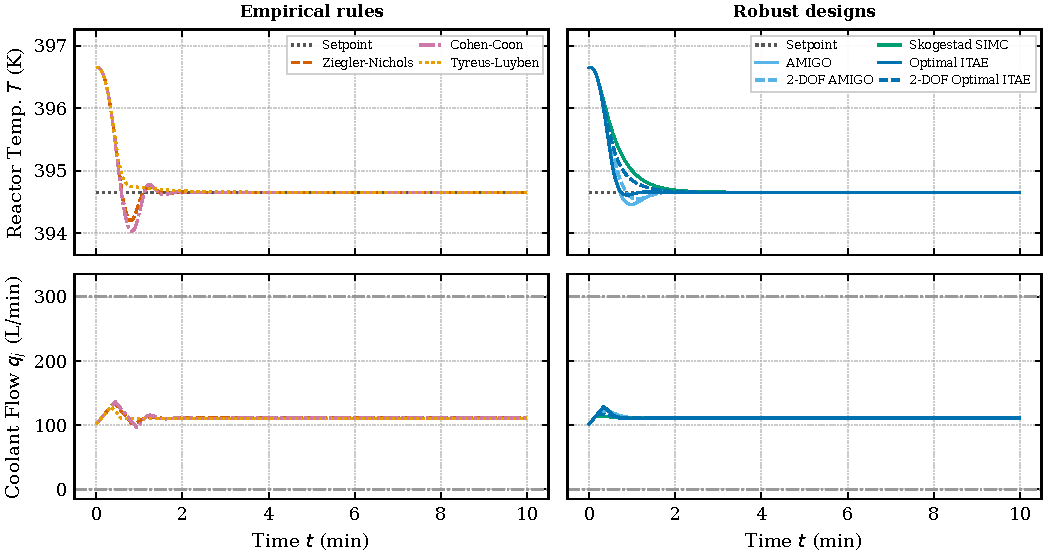
\includegraphics[width=0.92\textwidth]{figures/fig1_classical_benchmark.pdf}
    \caption{Nominal $-2$~K setpoint step (noise-free) under the valve limits $[0, 300]$~L/min and $80$~L/min$^2$, directional rule: empirical rules (left) and robust designs (right); reactor temperature (top) and coolant flow (bottom). The setpoint-weighted variants use $\beta = 0.5$, $\gamma = 0$ (Supplementary Section~\ref{supp:tuning}).}
    \label{fig:classical_benchmark}
\end{figure*}

\section{Anti-windup: full tables and discussion}\label{supp:aw}
Full versions of the results condensed in Section~\ref{subsec:ablation} of the main text.

\paragraph{Bound on the derivative term in Proposition~\ref{prop:latch}.} With $a = \tau_f/(\tau_f + \Delta t) \in (0, 1)$ and $K_p < 0$, Eq.~\eqref{eq:derivative_filtered} reads $D_k = a D_{k-1} + |K_p|T_d(T_k - T_{k-1})/(\tau_f + \Delta t)$. Since $(1-a)(\tau_f + \Delta t) = \Delta t$, induction gives, for $k > k_0$,
\begin{equation}
    |D_k| \le a^{k-k_0}|D_{k_0}| + (1 - a^{k-k_0})\,\frac{|K_p| T_d \bar\Delta}{\Delta t} \le \max\!\left(|D_{k_0}|, \frac{|K_p| T_d \bar\Delta}{\Delta t}\right) = \bar D,
    \label{eq:dbar}
\end{equation}
where $\bar\Delta$ bounds $|T_k - T_{k-1}|$; if $T_{k_0}$ also lies in the band of (H2), $\bar\Delta \le T_{sp} - T_\infty + \delta$. Hypothesis (H3) is therefore implied by (H2); \texttt{results/jpc/latch\_check.csv} evaluates $\bar D$ with this band bound.

\begin{table*}[t]
\centering
\footnotesize
\caption{Windup mechanism of the empirical rules on the $-2$~K step: lowest reactor temperature, time with the valve at its upper stop, final tracking error and largest command--valve discrepancy $\max|u_{\text{raw}}-u_{\text{act}}|$.}
\label{tab:antiwindup_mechanism}
\resizebox{\ifdim\width>\textwidth\textwidth\else\width\fi}{!}{%
\begin{tabular}{lccccc}
\toprule
Method & Anti-windup & \(T_{\min}\) (K) & Time at \(u_{\max}\) (min) & \(T(t_f)-T_{sp}\) (K) & \(\max|u_{\mathrm{raw}}-u_{\mathrm{act}}|\) (L/min) \\
\midrule
Ziegler-Nichols & None & 382.0 & 0.00 & +17.15 & 7775 \\
Ziegler-Nichols & Textbook & 377.8 & 3.86 & -16.72 & 4474 \\
Ziegler-Nichols & Directional (proposed) & 394.2 & 0.00 & +0.00 & 92 \\
Cohen-Coon & None & 382.8 & 0.00 & +8.52 & 8022 \\
Cohen-Coon & Textbook & 377.8 & 4.06 & -16.72 & 3540 \\
Cohen-Coon & Directional (proposed) & 394.0 & 0.00 & -0.00 & 105 \\
\bottomrule
\end{tabular}%
}
\end{table*}


\begin{table*}[t]
\centering
\footnotesize
\caption{IAE (K$\cdot$min) of the seven integrator policies of Table~\ref{tab:antiwindup_ablation} on a $-5$~K step, a $+5$~K step ($10$~min) and the noise-free load profile of Section~\ref{subsec:load_results} ($15$~min); valve $[0, 300]$~L/min, $S_{\max} = 80$~L/min$^2$; BC with $T_t = \sqrt{T_iT_d}$ and with the $T_t^{\mathrm{sel}}$ of Table~\ref{tab:antiwindup_tt_summary}.}
\label{tab:antiwindup_scenarios}
\resizebox{\ifdim\width>\textwidth\textwidth\else\width\fi}{!}{%
\begin{tabular}{lccccccccc}
\toprule
Scenario & Method & None & BC ($\sqrt{T_iT_d}$) & BC ($T_t^{\mathrm{sel}}$) & Sign-blind amp. & Amp. uncond. & Amp.+rate uncond. & Amp. direct. & Amp.+rate direct. (Eq.~\ref{eq:clamping_antiwindup}) \\
\midrule
$-5$ K step & Ziegler-Nichols & 81.26 & 3.63 & 3.42 & 205.97 & 22.50 & 3.56 & 22.50 & 3.33 \\
 & Cohen-Coon & 78.56 & 3.39 & 3.25 & 224.77 & 20.91 & 3.72 & 20.91 & 3.44 \\
 & Tyreus-Luyben & 5.51 & 4.42 & 3.32 & 5.51 & 5.51 & 4.01 & 5.51 & 3.55 \\
 & AMIGO & 41.34 & 3.32 & 3.32 & 43.74 & 31.17 & 3.32 & 31.17 & 3.32 \\
 & Skogestad SIMC & 3.78 & 4.94 & 3.80 & 3.78 & 3.78 & 4.41 & 3.78 & 4.41 \\
 & Optimal ITAE ($M_s^{\mathrm{FOPTD}} \leq 1.6$) & 14.29 & 3.53 & 3.16 & 14.29 & 14.29 & 3.26 & 14.29 & 3.26 \\
$+5$ K step & Ziegler-Nichols & 118.83 & 3.65 & 3.13 & 167.55 & 28.20 & 3.91 & 28.20 & 3.65 \\
 & Cohen-Coon & 116.02 & 3.28 & 2.91 & 166.99 & 26.00 & 4.58 & 26.00 & 4.39 \\
 & Tyreus-Luyben & 7.50 & 4.07 & 3.00 & 7.50 & 3.76 & 3.53 & 3.76 & 3.25 \\
 & AMIGO & 89.28 & 2.88 & 2.88 & 107.21 & 29.57 & 3.23 & 29.57 & 2.87 \\
 & Skogestad SIMC & 3.59 & 4.23 & 3.17 & 3.59 & 3.59 & 3.69 & 3.59 & 3.69 \\
 & Optimal ITAE ($M_s^{\mathrm{FOPTD}} \leq 1.6$) & 72.41 & 3.29 & 2.96 & 84.36 & 13.62 & 3.28 & 13.62 & 3.01 \\
Load (deterministic) & Ziegler-Nichols & 26.65 & 2.09 & 2.04 & 77.21 & 11.74 & 2.57 & 11.74 & 2.04 \\
 & Cohen-Coon & 26.14 & 1.99 & 1.97 & 72.02 & 11.29 & 2.56 & 11.29 & 1.98 \\
 & Tyreus-Luyben & 2.42 & 3.15 & 2.73 & 2.42 & 2.42 & 3.02 & 2.42 & 3.02 \\
 & AMIGO & 3.02 & 2.24 & 2.24 & 3.02 & 3.02 & 2.42 & 3.02 & 2.42 \\
 & Skogestad SIMC & 5.70 & 5.70 & 5.70 & 5.70 & 5.70 & 5.70 & 5.70 & 5.70 \\
 & Optimal ITAE ($M_s^{\mathrm{FOPTD}} \leq 1.6$) & 2.77 & 2.35 & 2.19 & 2.77 & 2.77 & 2.43 & 2.77 & 2.43 \\
\bottomrule
\end{tabular}%
}
\end{table*}


\paragraph{Why sign-blind clamping locks the valve at full cooling.} For ZN and CC the sign-blind rule is not merely ineffective, it is worse than no anti-windup (IAE $104.12$ and $102.67$ against $91.11$ and $87.37$~K$\cdot$min), and it fails in two steps. First, the slew limit lets the command run away from the valve position (by up to $4474$~L/min for ZN) while the valve is far from its stops. The condition ``$u_{\text{raw}} \ge u_{\max}$ and $e_k > 0$'' was written for a direct-acting loop. With $K_p < 0$, an overheated reactor ($T > T_{sp}$, $e_k < 0$) pushes the command \emph{up} towards $u_{\max}$; the product of the conditions is never true in that situation, so the integrator is never frozen when it should be and it winds up (the amplitude-only rule also misses the slew-rate cut). Second, the wound-up command drives the reactor below the setpoint ($e_k > 0$) while $u_{\text{raw}} \gg u_{\max}$ (the discrepancy is $3.5$--$4.5\times 10^{3}$~L/min); now both conditions hold and the rule \emph{freezes} the integrator, precisely when it must unwind. The valve reaches $u_{\max} = 300$~L/min at $t = 6.16$~min (ZN) and stays there until $t_f$, $3.86$ and $4.06$~min at the upper stop in Table~\ref{tab:antiwindup_mechanism}, and the reactor settles at the open-loop steady state of $q_j = 300$~L/min, $377.94$~K ($T(t_f) - T_{sp} = -16.72$~K for both rules, independent of the tuning, which is why both overshoot by the same $842.5\%$). With no anti-windup there is no latch: the valve never rests at its stop, but the wound-up integrator sustains a large oscillation (final error $+17.15$ and $+8.52$~K). The latch is the offset equilibrium $(T_\infty, u_{\max})$ of Proposition~\ref{prop:latch}: for ZN, $I^\star = 945$~L/min and the integrator of Fig.~\ref{fig:mechanism} settles above $3\times10^{3}$~L/min, so the condition of the proposition holds with a wide margin, whereas the directional rule is not frozen in that state (end of Section~\ref{subsec:clamping_rule}) and unwinds.

\paragraph{Factorial reading: the trigger, not the sign, restores the loop.} On the nominal step the amplitude-only variants, whether unconditional or directional, avoid the latch but still integrate through the rate-limited moves: IAE $22.10$ (ZN) and $20.60$~K$\cdot$min (CC), overshoots of $189.2\%$ and $181.2\%$. For TL, AMIGO, SIMC and Optimal ITAE the amplitude limit is never reached on this step, so every amplitude-triggered variant coincides with no anti-windup (and with sign-blind clamping); the equal columns of Table~\ref{tab:antiwindup_ablation} are not an artefact. Rate-aware triggers recover the tracking ($0.93$ and $1.10$~K$\cdot$min with the unconditional freeze, $0.94$ and $1.02$ with the directional one). Sign awareness is second order once the trigger is rate-aware: overshoots coincide for ZN, CC, AMIGO, SIMC and Optimal ITAE, the directional rule is faster for TL ($0.92$ against $1.07$) and for CC ($1.02$ against $1.10$), and the unconditional freeze is marginally faster for ZN ($0.93$ against $0.94$). The conclusion that the slew-rate trigger is the decisive ingredient does not depend on the step: Table~\ref{tab:antiwindup_scenarios} shows that on the $-5$~K step the amplitude-only variants leave ZN, CC, AMIGO and Optimal ITAE at IAE $22.50$, $20.91$, $31.17$ and $14.29$~K$\cdot$min against $3.33$, $3.44$, $3.32$ and $3.26$ with the rate-aware directional rule, and on the $+5$~K step at $28.20$, $26.00$, $29.57$ and $13.62$ against $3.65$, $4.39$, $2.87$ and $3.01$. Hence AMIGO and Optimal ITAE, whose nominal step does not expose the problem, are also affected by large moves. Sign-blind clamping is worse than no anti-windup for the empirical rules at both signs ($205.97$ and $224.77$ against $81.26$ and $78.56$ at $-5$~K) and also on the load profile ($77.21$ and $72.02$ against $26.65$ and $26.14$).

\paragraph{Back-calculation and its tracking constant.} Fig.~\ref{fig:tt_curve} scans $T_t$ from $0.525\,\Delta t$ to $10\,T_i$ for the three steps. The physical range of the tracking constant is $T_d \le T_t \le T_i$; outside it the scheme is either not meant to work or numerically degenerate, because the discrete update multiplies $I$ by $1 - \Delta t/T_t$, which over-corrects for $T_t < \Delta t$ and diverges below $\Delta t/2$. A scan at $0.1\,T_t$ (nominal IAE $18.56$~K$\cdot$min for both ZN and CC, \texttt{results/jpc/antiwindup\_tt\_curve.csv}) and at $10\,T_t$ lies outside that range and is not evidence against back-calculation: at $0.1\,T_t$ the ratio $\Delta t/T_t$ is $2.14$ (ZN) and $2.36$ (CC), the valve stays within $1.6$~L/min of its bias for the whole step for both rules and the IAE is the same ($18.56$), and at $10\,T_t$ the constant exceeds $T_i$. These two limits belong to the explicit Euler discretization of Eq.~\eqref{eq:back_calculation}. With the exact zero-order-hold factor, $I_k = I_{k-1} + \delta I_k + (1 - e^{-\Delta t/T_t})(u_{\text{act},k-1} - u_{\text{raw},k-1})$, the factor stays in $(0, 1)$ for every $T_t > 0$ and the scheme neither over-corrects nor diverges: at $0.1\sqrt{T_iT_d}$ the IAE of ZN and CC on the $-2$~K step falls from $\vexZNeuler$ and $\vexCCeuler$ (Euler, valve chattering at the slew limit, TV $\vexZNTVeuler$~L/min) to $\vexZNexact$ and $\vexCCexact$~K$\cdot$min, and the loops with $1 < \Delta t/T_t < 2$ also improve (Table~\ref{tab:exact_backcalc}). A fair comparison needs one $T_t$ per loop, not the best $T_t$ per step, which uses information a practitioner does not have. Two declared criteria are used (Table~\ref{tab:antiwindup_tt_summary}): $T_t^{\mathrm{mm}}$ minimizes, inside $[T_d, T_i]$, the largest ratio of the back-calculation IAE to the directional-rule IAE over the three steps (minimax), and $T_t^{\mathrm{cv}}$ is chosen on the $-2$~K design step only and judged on $\pm 5$~K. With $T_t^{\mathrm{mm}}$ the worst ratio is $1.02$, $0.94$, $0.94$, $1.00$, $0.90$ and $1.01$ for ZN, CC, TL, AMIGO, SIMC and Optimal ITAE: a back-calculation with one well-chosen constant per loop is at most $2\%$ worse than the directional rule in any step and up to $10\%$ better. The design-step choice $T_t^{\mathrm{cv}}$ coincides with $T_t^{\mathrm{mm}}$ for five of the six loops (AMIGO: $0.121$ against $0.139$~min) and its worst ratio on $\pm 5$~K is $1.02$ or lower, so the choice transfers. The usual defaults are worse: $T_t = \sqrt{T_iT_d}$ gives worst ratios of $1.09$, $0.98$, $1.37$, $1.00$, $1.15$ and $1.20$ and $T_t = T_i$, the value associated with conditioning techniques \cite{peng1996nonlinear}, $1.97$, $1.90$, $1.01$, $1.26$, $0.90$ and $1.18$ (Table~\ref{tab:antiwindup_tt_sweep} lists the IAE per step). The directional rule is therefore not better than a back-calculation whose constant was chosen with care, and the choice of $T_t$ matters by up to a factor of two among the usual defaults; the advantage of the directional rule is that it needs no per-loop constant. It is not free of assumptions either: its behaviour depends on the slew limit $S_{\max}$ and on the sampling interval $\Delta t$ through $u_{\text{act}}$, which the next paragraphs map. Dynamic compensators designed by LMI \cite{galeani2009tutorial, lerch2021antiwindup} are not part of the comparison: they need a plant model and a design step that are outside the scope of an implementation study of PID loops.

\begin{table*}[t]
\centering
\footnotesize
\caption{IAE (K$\cdot$min) of the directional rule (``dir.'') and of back-calculation with $T_t^{\mathrm{mm}}$ and $T_t^{\mathrm{sel}}$ (Table~\ref{tab:antiwindup_tt_summary}), $T_t = \sqrt{T_iT_d}$ and $T_t = T_i$ (the value associated with conditioning techniques \cite{peng1996nonlinear}). The full curves are in Fig.~\ref{fig:tt_curve}.}
\label{tab:antiwindup_tt_sweep}
\resizebox{\ifdim\width>\textwidth\textwidth\else\width\fi}{!}{%
\begin{tabular}{lcccccc}
\toprule
Method & Step & IAE dir. & IAE $T_t^{\mathrm{mm}}$ & IAE $\sqrt{T_iT_d}$ & IAE $T_t=T_i$ & IAE $T_t^{\mathrm{sel}}$ \\
\midrule
Ziegler-Nichols & $-2$ K & 0.94 & 0.88 & 0.97 & 1.66 & 0.88 \\
 & $-5$ K & 3.33 & 3.42 & 3.63 & 4.92 & 3.42 \\
 & $+5$ K & 3.65 & 3.13 & 3.65 & 7.20 & 3.13 \\
Cohen-Coon & $-2$ K & 1.02 & 0.82 & 0.87 & 1.81 & 0.82 \\
 & $-5$ K & 3.44 & 3.25 & 3.39 & 4.99 & 3.25 \\
 & $+5$ K & 4.39 & 2.91 & 3.28 & 8.36 & 2.91 \\
Tyreus-Luyben & $-2$ K & 0.92 & 0.83 & 1.26 & 0.87 & 0.83 \\
 & $-5$ K & 3.55 & 3.32 & 4.42 & 3.30 & 3.32 \\
 & $+5$ K & 3.25 & 3.00 & 4.07 & 3.29 & 3.00 \\
AMIGO & $-2$ K & 0.93 & 0.92 & 0.92 & 1.00 & 0.92 \\
 & $-5$ K & 3.32 & 3.32 & 3.32 & 3.51 & 3.32 \\
 & $+5$ K & 2.87 & 2.88 & 2.88 & 3.61 & 2.88 \\
Skogestad SIMC & $-2$ K & 1.29 & 1.15 & 1.47 & 1.15 & 1.15 \\
 & $-5$ K & 4.41 & 3.80 & 4.94 & 3.80 & 3.80 \\
 & $+5$ K & 3.69 & 3.17 & 4.23 & 3.17 & 3.17 \\
Optimal ITAE ($M_s^{\mathrm{FOPTD}} \leq 1.6$) & $-2$ K & 0.83 & 0.83 & 0.99 & 0.92 & 0.83 \\
 & $-5$ K & 3.26 & 3.16 & 3.53 & 3.44 & 3.16 \\
 & $+5$ K & 3.01 & 2.96 & 3.29 & 3.56 & 2.96 \\
\bottomrule
\end{tabular}%
}
\end{table*}


\begin{table*}[t]
\centering
\footnotesize
\caption{Back-calculation with $T_t^{\mathrm{cv}}$ (BC) against the directional rule (dir., Eq.~\eqref{eq:clamping_antiwindup}) on the three steps: IAE (K$\cdot$min), valve travel TV and overshoot $M_p$.}
\label{tab:antiwindup_tt_tvmp}
\resizebox{\ifdim\width>\textwidth\textwidth\else\width\fi}{!}{%
\begin{tabular}{lccccccc}
\toprule
Method & Step & IAE dir. & IAE BC & TV dir. (L/min) & TV BC (L/min) & \(M_p\) dir. (\%) & \(M_p\) BC (\%) \\
\midrule
Ziegler-Nichols & $-2$ K & 0.94 & 0.88 & 81.9 & 70.8 & 22.6 & 15.0 \\
 & $-5$ K & 3.33 & 3.42 & 123.2 & 130.6 & 11.9 & 14.9 \\
 & $+5$ K & 3.65 & 3.13 & 161.2 & 117.6 & 33.6 & 20.6 \\
Cohen-Coon & $-2$ K & 1.02 & 0.82 & 104.0 & 61.9 & 31.0 & 6.0 \\
 & $-5$ K & 3.44 & 3.25 & 150.1 & 115.2 & 15.6 & 9.1 \\
 & $+5$ K & 4.39 & 2.91 & 241.9 & 101.2 & 40.8 & 11.3 \\
Tyreus-Luyben & $-2$ K & 0.92 & 0.83 & 48.8 & 52.1 & 0.0 & 0.0 \\
 & $-5$ K & 3.55 & 3.32 & 90.8 & 89.5 & 0.0 & 0.0 \\
 & $+5$ K & 3.25 & 3.00 & 112.4 & 103.9 & 11.1 & 13.0 \\
AMIGO & $-2$ K & 0.93 & 0.92 & 40.4 & 36.8 & 9.7 & 8.0 \\
 & $-5$ K & 3.32 & 3.32 & 70.3 & 72.1 & 4.9 & 5.6 \\
 & $+5$ K & 2.87 & 2.88 & 70.0 & 65.5 & 3.1 & 3.1 \\
Skogestad SIMC & $-2$ K & 1.29 & 1.15 & 15.7 & 18.9 & 0.0 & 0.3 \\
 & $-5$ K & 4.41 & 3.80 & 30.7 & 42.5 & 0.0 & 0.0 \\
 & $+5$ K & 3.69 & 3.17 & 35.4 & 47.8 & 0.0 & 0.9 \\
Optimal ITAE ($M_s^{\mathrm{FOPTD}} \leq 1.6$) & $-2$ K & 0.83 & 0.83 & 48.6 & 50.1 & 2.2 & 4.4 \\
 & $-5$ K & 3.26 & 3.16 & 76.7 & 84.1 & 0.0 & 0.5 \\
 & $+5$ K & 3.01 & 2.96 & 105.0 & 100.8 & 8.7 & 12.5 \\
\bottomrule
\end{tabular}%
}
\end{table*}


\begin{table*}[t]
\centering
\footnotesize
\caption{Back-calculation at $T_t = 0.1\sqrt{T_iT_d}$, below the physical range: tracking term discretized by explicit Euler, $(\Delta t/T_t)(u_{\text{act},k-1} - u_{\text{raw},k-1})$ (Eq.~\eqref{eq:back_calculation}), and by the exact zero-order-hold factor $(1 - e^{-\Delta t/T_t})(u_{\text{act},k-1} - u_{\text{raw},k-1})$; IAE in K$\cdot$min.}
\label{tab:exact_backcalc}
\resizebox{\ifdim\width>\textwidth\textwidth\else\width\fi}{!}{%
\begin{tabular}{lccccccc}
\toprule
Method & \(T_t\) (min) & \(\Delta t/T_t\) & Step & IAE Euler & IAE exact & TV Euler (L/min) & TV exact (L/min) \\
\midrule
Ziegler-Nichols & 0.0093 & 2.14 & $-2$ K & 18.56 & 0.87 & 801.6 & 67.2 \\
 &  &  & $-5$ K & 48.56 & 3.39 & 801.6 & 125.9 \\
 &  &  & $+5$ K & 48.54 & 3.04 & 801.6 & 108.2 \\
Cohen-Coon & 0.0085 & 2.36 & $-2$ K & 18.56 & 0.82 & 801.6 & 60.9 \\
 &  &  & $-5$ K & 48.56 & 3.24 & 801.6 & 113.5 \\
 &  &  & $+5$ K & 48.54 & 2.90 & 801.6 & 98.6 \\
Tyreus-Luyben & 0.0209 & 0.96 & $-2$ K & 1.81 & 1.76 & 10.9 & 11.2 \\
 &  &  & $-5$ K & 4.98 & 4.98 & 30.0 & 30.0 \\
 &  &  & $+5$ K & 4.75 & 4.75 & 23.7 & 23.8 \\
AMIGO & 0.0121 & 1.65 & $-2$ K & 1.16 & 0.96 & 36.3 & 29.6 \\
 &  &  & $-5$ K & 3.92 & 3.33 & 76.4 & 66.9 \\
 &  &  & $+5$ K & 3.51 & 2.92 & 66.2 & 56.8 \\
Skogestad SIMC & 0.0141 & 1.42 & $-2$ K & 2.22 & 1.98 & 14.1 & 10.9 \\
 &  &  & $-5$ K & 6.17 & 5.68 & 34.7 & 30.0 \\
 &  &  & $+5$ K & 5.46 & 4.97 & 28.5 & 23.8 \\
Optimal ITAE ($M_s^{\mathrm{FOPTD}} \leq 1.6$) & 0.0122 & 1.65 & $-2$ K & 1.36 & 1.13 & 30.4 & 21.3 \\
 &  &  & $-5$ K & 4.27 & 3.61 & 58.2 & 48.7 \\
 &  &  & $+5$ K & 4.06 & 3.40 & 53.4 & 44.0 \\
\bottomrule
\end{tabular}%
}
\end{table*}


\paragraph{Freeze test at the current sample.} Eq.~\eqref{eq:clamping_antiwindup} decides the freeze on the residual of the previous sample. A predictor-corrector variant decides it at the current sample without an algebraic loop: it forms the trial command $\hat u_{\text{raw},k} = u_{\text{bias}} + P_k + I_{k-1} + \delta I_k + D_k$, passes it through the valve map from the previous position, $\hat u_{\text{act},k} = \operatorname{rate}(\operatorname{sat}(\hat u_{\text{raw},k}))$, and sets $I_k = I_{k-1}$ if $(\hat u_{\text{raw},k} - \hat u_{\text{act},k})\,\delta I_k > 0$ (\texttt{AntiWindupMethod.CLAMPING\_PREDICTIVE}). Table~\ref{tab:predictive_clamping} compares the two on the three steps. For TL, AMIGO, SIMC and Optimal ITAE the IAE changes by at most $\vpcrestmaxpct\%$; for ZN and CC the one-sample delay matters on the $+5$~K step, where the test at $k$ lowers the IAE from $\vpcZNfiveold$ to $\vpcZNfivenew$ and from $\vpcCCfiveold$ to $\vpcCCfivenew$~K$\cdot$min (largest changes $\vpcZNmaxpct\%$ and $\vpcCCmaxpct\%$). The conclusions do not change: SIMC remains worse than no anti-windup on all three steps, and with the test at $k$ as reference the worst ratio of back-calculation with $T_t^{\mathrm{cv}}$ on $\pm 5$~K lies between $\vpcttcvmin$ and $\vpcttcvmax$ (against $\vttcvmin$ and $\vttcvmax$ with Eq.~\eqref{eq:clamping_antiwindup}).

\begin{table*}[t]
\centering
\footnotesize
\caption{Directional rule with the freeze decision taken on the residual of the previous sample (Eq.~\eqref{eq:clamping_antiwindup}, ``$k-1$'') and on a predictor-corrector trial at the current sample (``$k$''): IAE (K$\cdot$min), TV (L/min) and overshoot (\%) on the three steps, valve $[0, 300]$~L/min, $S_{\max} = 80$~L/min$^2$.}
\label{tab:predictive_clamping}
\resizebox{\ifdim\width>\textwidth\textwidth\else\width\fi}{!}{%
\begin{tabular}{lcccccccc}
\toprule
Method & Step & IAE, \(k-1\) & IAE, \(k\) & TV, \(k-1\) & TV, \(k\) & \(M_p\), \(k-1\) & \(M_p\), \(k\) & \(\Delta\)IAE (\%) \\
\midrule
Ziegler-Nichols & $-2$ K & 0.940 & 0.936 & 81.9 & 80.7 & 22.6 & 22.2 & -0.34 \\
 & $-5$ K & 3.333 & 3.388 & 123.2 & 125.4 & 11.9 & 13.9 & +1.67 \\
 & $+5$ K & 3.652 & 3.435 & 161.2 & 154.4 & 33.6 & 26.5 & -5.94 \\
Cohen-Coon & $-2$ K & 1.017 & 1.007 & 104.0 & 105.8 & 31.0 & 29.2 & -0.98 \\
 & $-5$ K & 3.443 & 3.360 & 150.1 & 148.2 & 15.6 & 11.9 & -2.39 \\
 & $+5$ K & 4.389 & 4.078 & 241.9 & 223.2 & 40.8 & 33.6 & -7.08 \\
Tyreus-Luyben & $-2$ K & 0.917 & 0.912 & 48.8 & 48.9 & 0.0 & 0.0 & -0.59 \\
 & $-5$ K & 3.547 & 3.551 & 90.8 & 89.6 & 0.0 & 0.0 & +0.13 \\
 & $+5$ K & 3.249 & 3.248 & 112.4 & 112.9 & 11.1 & 10.9 & -0.05 \\
AMIGO & $-2$ K & 0.925 & 0.928 & 40.4 & 41.7 & 9.7 & 10.3 & +0.24 \\
 & $-5$ K & 3.324 & 3.324 & 70.3 & 68.3 & 4.9 & 5.0 & +0.02 \\
 & $+5$ K & 2.873 & 2.879 & 70.0 & 66.9 & 3.1 & 3.4 & +0.20 \\
Skogestad SIMC & $-2$ K & 1.288 & 1.270 & 15.7 & 16.1 & 0.0 & 0.0 & -1.40 \\
 & $-5$ K & 4.405 & 4.370 & 30.7 & 31.2 & 0.0 & 0.0 & -0.80 \\
 & $+5$ K & 3.687 & 3.653 & 35.4 & 35.5 & 0.0 & 0.0 & -0.92 \\
Optimal ITAE ($M_s^{\mathrm{FOPTD}} \leq 1.6$) & $-2$ K & 0.827 & 0.832 & 48.6 & 46.4 & 2.2 & 0.9 & +0.54 \\
 & $-5$ K & 3.262 & 3.264 & 76.7 & 76.7 & 0.0 & 0.0 & +0.05 \\
 & $+5$ K & 3.007 & 3.009 & 105.0 & 105.0 & 8.7 & 8.4 & +0.05 \\
\bottomrule
\end{tabular}%
}
\end{table*}


\paragraph{Regime map: where the slew-rate trigger matters.} The gains were designed at $S_{\max} = 80$~L/min$^2$; Fig.~\ref{fig:smax_map} and Table~\ref{tab:smax_map} repeat the $-2$~K step for $S_{\max}$ from $20$ to $320$~L/min$^2$ ($S_{\max} = 320$ is a full stroke in $0.94$~min) with the gains fixed. For ZN and CC the amplitude-only variants are $7.4$ to $38$ times worse than the rate-aware rule at every $S_{\max}$, because the amplitude limit is reached and the integrator winds up during the rate-limited ramp; sign-blind clamping latches at $-16.7$~K for $S_{\max} \ge 60$ (at $45$: $-14.9$ and $-16.0$~K) and oscillates at $20$~L/min$^2$ (ZN: $+32.5$~K). The ZN value of $+54.2$~K at $240$~L/min$^2$ is not an oscillation: the command overshoots below $u_{\min}$ while the reactor is above the setpoint, the condition ``$u_{\text{raw}} \le u_{\min}$ and $e_k < 0$'' freezes the integrator, and the valve stays closed for $\vsbZNlowtime$~min, the mirror image at the lower stop of the latch of Proposition~\ref{prop:latch}; the reactor heats towards its closed-valve state and is still rising at $\vsbZNlowrate$~K/min at $t_f$ (\texttt{results/jpc/smax\_signblind\_diagnostics.csv}). For AMIGO and Optimal ITAE the ratio is $11.5$ and $9.3$ at $20$~L/min$^2$, $1.7$ and $1.8$ at the benchmark value and $1.1$ and $1.3$ at $320$: the trigger matters when the valve is slow compared with what the loop demands, and fades as $S_{\max}$ grows. The AMIGO ratio is not monotone ($11.5$, $14.7$, $14.4$ at $20$, $30$, $45$ and then $2.7$ at $60$~L/min$^2$): the valve never reaches an amplitude stop for AMIGO (largest opening $153.5$~L/min, \texttt{results/jpc/smax\_amigo\_diagnostics.csv}), the amplitude-only IAE ($18.0$, $19.22$, $16.02$) is set by a large oscillation of the loop wound up during the ramp, while the rate-aware IAE falls smoothly; between $45$ and $60$~L/min$^2$ the command--valve discrepancy drops from $111$ to $41$~L/min and the oscillation disappears (IAE $2.71$). The threshold is a property of this loop and step, not a general value. For TL the ratio is between $1.2$ and $2.1$. For SIMC the trigger helps only at $20$~L/min$^2$ (ratio $\vSIMCratiotwenty$) and makes the loop worse at every faster valve ($\vSIMCratioff$, $\vSIMCratioeighty$ and $\vSIMCratiolast$ at $45$, $80$ and $320$~L/min$^2$): SIMC is the counterexample discussed in Section~\ref{subsec:regime}. Re-optimizing the Optimal ITAE gains at each $S_{\max}$ (Table~\ref{tab:smax_retuned}) keeps $K_p$ near $-23.5$ and moves $T_i$ from $0.36$ to $0.63$~min; the ratio is $11.3$, $14.9$, $6.0$, $3.0$, $1.8$, $1.5$, $1.5$, $1.3$ and $1.3$, larger than with fixed gains at $45$ and $60$~L/min$^2$ ($6.0$ and $3.0$ against $3.5$ and $2.4$) and equal from $80$ up, so the conclusion does not depend on the gains having been designed at $80$~L/min$^2$. The rate-aware rule is therefore free of a tuning constant but not of its environment: its benefit is a function of $S_{\max}$ and of the loop.

\begin{table*}[t]
\centering
\footnotesize
\caption{Regime map over the valve slew-rate limit ($-2$~K step, gains designed at $S_{\max} = 80$~L/min$^2$). First row of each tuning: IAE of amplitude-only directional clamping over IAE of the rate-aware rule (values near $1$: the rate trigger is irrelevant); second: IAE of the rate-aware rule; third: final error of sign-blind clamping ($\approx -16.7$~K: valve latched at full cooling).}
\label{tab:smax_map}
\resizebox{\ifdim\width>\textwidth\textwidth\else\width\fi}{!}{%
\begin{tabular}{lcccccccccc}
\toprule
Method & Quantity & $S_{\max}=20$ & $S_{\max}=30$ & $S_{\max}=45$ & $S_{\max}=60$ & $S_{\max}=80$ & $S_{\max}=120$ & $S_{\max}=160$ & $S_{\max}=240$ & $S_{\max}=320$ \\
\midrule
Ziegler-Nichols & $\mathrm{IAE}_{\mathrm{amp}}/\mathrm{IAE}_{\mathrm{rate}}$ & 7.9 & 11.5 & 15.6 & 19.7 & 23.5 & 30.8 & 35.7 & 38.3 & 36.3 \\
 & IAE rate-aware (K$\cdot$min) & 1.62 & 1.38 & 1.16 & 1.06 & 0.94 & 0.77 & 0.70 & 0.63 & 0.60 \\
 & Sign-blind $T(t_f)-T_{sp}$ (K) & +32.5 & +1.9 & -14.9 & -16.7 & -16.7 & -16.7 & -16.7 & +54.2 & -16.7 \\
Cohen-Coon & $\mathrm{IAE}_{\mathrm{amp}}/\mathrm{IAE}_{\mathrm{rate}}$ & 7.4 & 10.2 & 13.5 & 16.8 & 20.3 & 26.6 & 32.7 & 35.5 & 37.7 \\
 & IAE rate-aware (K$\cdot$min) & 1.70 & 1.47 & 1.26 & 1.17 & 1.02 & 0.85 & 0.72 & 0.62 & 0.55 \\
 & Sign-blind $T(t_f)-T_{sp}$ (K) & +30.6 & -3.3 & -16.0 & -16.7 & -16.7 & -16.7 & -16.7 & -16.3 & -16.7 \\
Tyreus-Luyben & $\mathrm{IAE}_{\mathrm{amp}}/\mathrm{IAE}_{\mathrm{rate}}$ & 2.1 & 1.8 & 1.5 & 1.4 & 1.4 & 1.3 & 1.3 & 1.3 & 1.2 \\
 & IAE rate-aware (K$\cdot$min) & 1.67 & 1.39 & 1.16 & 1.04 & 0.92 & 0.79 & 0.69 & 0.59 & 0.55 \\
 & Sign-blind $T(t_f)-T_{sp}$ (K) & -0.0 & -0.0 & -0.0 & -0.0 & -0.0 & -0.0 & -0.0 & -0.0 & -0.0 \\
AMIGO & $\mathrm{IAE}_{\mathrm{amp}}/\mathrm{IAE}_{\mathrm{rate}}$ & 11.5 & 14.7 & 14.4 & 2.7 & 1.7 & 1.4 & 1.3 & 1.2 & 1.1 \\
 & IAE rate-aware (K$\cdot$min) & 1.57 & 1.30 & 1.11 & 1.01 & 0.93 & 0.84 & 0.79 & 0.75 & 0.72 \\
 & Sign-blind $T(t_f)-T_{sp}$ (K) & +2.5 & -0.4 & -2.5 & -0.0 & -0.0 & -0.0 & -0.0 & -0.0 & -0.0 \\
Skogestad SIMC & $\mathrm{IAE}_{\mathrm{amp}}/\mathrm{IAE}_{\mathrm{rate}}$ & 1.0 & 0.9 & 0.9 & 0.8 & 0.8 & 0.9 & 0.9 & 0.9 & 0.9 \\
 & IAE rate-aware (K$\cdot$min) & 1.94 & 1.69 & 1.48 & 1.36 & 1.29 & 1.17 & 1.13 & 1.06 & 1.06 \\
 & Sign-blind $T(t_f)-T_{sp}$ (K) & -0.0 & -0.0 & -0.0 & -0.0 & -0.0 & -0.0 & -0.0 & -0.0 & -0.0 \\
Optimal ITAE ($M_s^{\mathrm{FOPTD}} \leq 1.6$) & $\mathrm{IAE}_{\mathrm{amp}}/\mathrm{IAE}_{\mathrm{rate}}$ & 9.3 & 9.6 & 3.5 & 2.4 & 1.8 & 1.5 & 1.5 & 1.3 & 1.3 \\
 & IAE rate-aware (K$\cdot$min) & 1.59 & 1.30 & 1.07 & 0.93 & 0.83 & 0.72 & 0.66 & 0.61 & 0.58 \\
 & Sign-blind $T(t_f)-T_{sp}$ (K) & +0.3 & +0.2 & +0.0 & -0.0 & +0.0 & -0.0 & -0.0 & -0.0 & -0.0 \\
\bottomrule
\end{tabular}%
}
\end{table*}


\begin{figure*}[t]
    \centering
    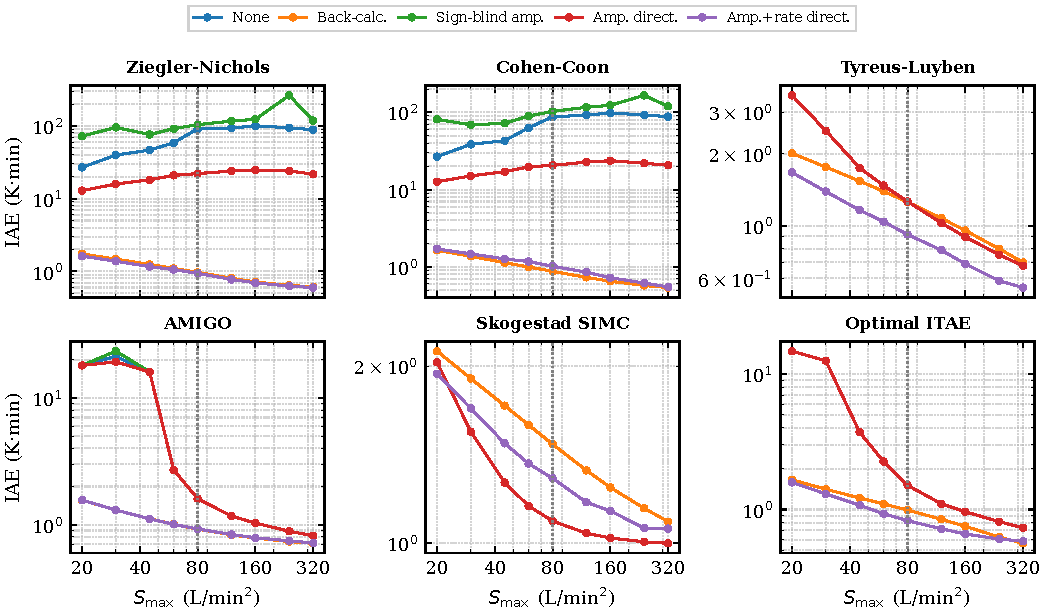
\includegraphics[width=0.92\textwidth]{figures/fig_smax_map.pdf}
    \caption{IAE of the $-2$~K step against the valve slew-rate limit for five integrator policies and six loops (gains fixed; dotted: benchmark $S_{\max} = 80$~L/min$^2$).}
    \label{fig:smax_map}
\end{figure*}

\begin{table*}[t]
\centering
\footnotesize
\caption{Optimal ITAE ($M_s^{\mathrm{FOPTD}} \le 1.6$) re-optimized at each slew-rate limit (multi-start from the $S_{\max} = 80$ optimum and the default guess, one restart): gains and IAE ($-2$~K step) of amplitude-only directional clamping and of the rate-aware rule. Compare with the fixed-gain map of Table~\ref{tab:smax_map}.}
\label{tab:smax_retuned}
\resizebox{\ifdim\width>\textwidth\textwidth\else\width\fi}{!}{%
\begin{tabular}{lcccccc}
\toprule
\(S_{\max}\) (L/min$^2$) & \(K_p\) & \(T_i\) (min) & \(T_d\) (min) & IAE amp.-only & IAE rate-aware & ratio \\
\midrule
20 & -22.9 & 0.364 & 0.036 & 17.26 & 1.53 & 11.3 \\
30 & -23.3 & 0.382 & 0.033 & 18.70 & 1.26 & 14.9 \\
45 & -23.2 & 0.417 & 0.036 & 6.28 & 1.05 & 6.0 \\
60 & -23.5 & 0.429 & 0.032 & 2.78 & 0.93 & 3.0 \\
80 & -23.6 & 0.465 & 0.032 & 1.51 & 0.83 & 1.8 \\
120 & -23.5 & 0.499 & 0.033 & 1.09 & 0.72 & 1.5 \\
160 & -23.5 & 0.501 & 0.032 & 0.95 & 0.65 & 1.5 \\
240 & -23.3 & 0.564 & 0.034 & 0.78 & 0.58 & 1.3 \\
320 & -23.4 & 0.626 & 0.033 & 0.69 & 0.54 & 1.3 \\
\bottomrule
\end{tabular}%
}
\end{table*}


\paragraph{Rate demand.} Table~\ref{tab:rate_demand} gives, for the six loops and the three steps at the benchmark limit, the ratio of the regime map and the rate demand $\rho = \max_k|u_k - u_{k-1}|/(S_{\max}\Delta t)$ of the same loop simulated with the slew limit removed and the amplitude limit kept (the setpoint kick at $t = 0$, common to every loop, is excluded). $\rho$ is an ex-ante quantity: it uses the IAE of neither rule and needs only one simulation of the loop without the slew limit. At $S_{\max} = 80$~L/min$^2$ the demand of SIMC is at most $\vrhoSIMCmaxeighty$ and that of the other loops at least $\vrhoothersmineighty$, but over the whole grid of $\vncases$ cases ($\texttt{results/jpc/rate\_demand\_grid.csv}$) the demand does not separate SIMC: with $\rho \ge 1$ the trigger improved the loop in $\vnrhohihelp$ of $\vnrhohi$ cases (worst ratio $\vrhohiratiomin$), whereas with $\rho < 1$ the ratio ranged from $\vrholoratiomin$ to $\vrholoratiomax$; every one of the $\vnrholohurt$ cases made worse with $\rho < 1$ is SIMC, yet \vrhohelplowloop{} at $\vrhohelplowsmax$~L/min$^2$ still gains ($\vrhohelplowratio$) with $\rho = \vrhohelplow$. The demand thus gives a heuristic that was sufficient on this reactor ($\rho \ge 1$: switch the trigger on), not a separating criterion; it is model-based and was observed without measurement noise. Table~\ref{tab:rate_demand_check} applies it to conditions not used to draw it: all $\vchkrhohi$ loops with $\rho \ge 1$ improve with the trigger, and of the $\vchkrholo$ with $\rho < 1$, AMIGO gains and SIMC loses.

\begin{table*}[t]
\centering
\footnotesize
\caption{The rate-demand rule outside the conditions on which it was observed: $-2$~K step, $S_{\max} = 80$~L/min$^2$, at the second operating point (re-tuned loops) and with valve deadbands of $3$ and $6$~L/min. $\rho$ as in Table~\ref{tab:rate_demand} (deadband kept, slew limit removed); ratio above $1$: the rate trigger improves the loop.}
\label{tab:rate_demand_check}
\resizebox{\ifdim\width>\textwidth\textwidth\else\width\fi}{!}{%
\begin{tabular}{lccc}
\toprule
Condition & Method & \(\rho\) & \(\mathrm{IAE}_{\mathrm{amp}}/\mathrm{IAE}_{\mathrm{rate}}\) \\
\midrule
$q_{j,ss} = 150$ & Ziegler-Nichols & 4.63 & 16.07 \\
 & Cohen-Coon & 6.27 & 14.72 \\
 & Tyreus-Luyben & 2.90 & 1.18 \\
 & AMIGO & 1.16 & 2.03 \\
 & Skogestad SIMC & 0.35 & 0.82 \\
deadband 3 L/min & Ziegler-Nichols & 5.22 & 18.35 \\
 & Cohen-Coon & 6.84 & 16.28 \\
 & Tyreus-Luyben & 2.82 & 1.38 \\
 & AMIGO & 0.87 & 1.75 \\
 & Skogestad SIMC & 0.21 & 0.87 \\
 & Optimal ITAE ($M_s^{\mathrm{FOPTD}} \leq 1.6$) & 1.62 & 1.88 \\
deadband 6 L/min & Ziegler-Nichols & 5.35 & 15.03 \\
 & Cohen-Coon & 6.96 & 13.10 \\
 & Tyreus-Luyben & 2.84 & 1.41 \\
 & AMIGO & 0.94 & 1.75 \\
 & Skogestad SIMC & 0.22 & 0.81 \\
 & Optimal ITAE ($M_s^{\mathrm{FOPTD}} \leq 1.6$) & 1.68 & 2.09 \\
\bottomrule
\end{tabular}%
}
\end{table*}


\begin{table*}[t]
\centering
\footnotesize
\caption{Rate demand and the slew-rate trigger at $S_{\max} = 80$~L/min$^2$: IAE of amplitude-only over that of rate-aware directional clamping (below $1$: the trigger makes the loop worse), peak rate demanded by the same loop with the slew limit removed relative to the limit, $\rho = \max_k |u_k - u_{k-1}|/(S_{\max}\Delta t)$ (setpoint kick at $t = 0$ excluded), and time spent slew-limited under the rate-aware rule. The full grid over $S_{\max}$ is in \texttt{results/jpc/rate\_demand\_grid.csv}.}
\label{tab:rate_demand}
\resizebox{\ifdim\width>\textwidth\textwidth\else\width\fi}{!}{%
\begin{tabular}{lcccc}
\toprule
Method & Step & \(\mathrm{IAE}_{\mathrm{amp}}/\mathrm{IAE}_{\mathrm{rate}}\) & \(\rho\) & slew-limited (min) \\
\midrule
Ziegler-Nichols & $-2$ K & 23.52 & 5.11 & 0.76 \\
 & $-5$ K & 6.75 & 15.36 & 1.28 \\
 & $+5$ K & 7.72 & 10.63 & 1.76 \\
Cohen-Coon & $-2$ K & 20.26 & 6.72 & 1.10 \\
 & $-5$ K & 6.07 & 11.03 & 1.66 \\
 & $+5$ K & 5.92 & 13.99 & 2.80 \\
Tyreus-Luyben & $-2$ K & 1.38 & 2.75 & 0.54 \\
 & $-5$ K & 1.55 & 5.89 & 1.04 \\
 & $+5$ K & 1.16 & 8.70 & 1.32 \\
AMIGO & $-2$ K & 1.73 & 0.83 & 0.28 \\
 & $-5$ K & 9.38 & 2.10 & 0.58 \\
 & $+5$ K & 10.29 & 3.73 & 0.58 \\
Skogestad SIMC & $-2$ K & 0.85 & 0.21 & 0.14 \\
 & $-5$ K & 0.86 & 0.52 & 0.34 \\
 & $+5$ K & 0.97 & 0.51 & 0.34 \\
Optimal ITAE ($M_s^{\mathrm{FOPTD}} \leq 1.6$) & $-2$ K & 1.82 & 1.55 & 0.32 \\
 & $-5$ K & 4.38 & 2.93 & 0.64 \\
 & $+5$ K & 4.53 & 5.37 & 1.06 \\
\bottomrule
\end{tabular}%
}
\end{table*}


\paragraph{Valve deadband.} The deadband is a backlash (play) operator of width $b$ placed after the amplitude and slew limits, exactly as \texttt{\_Deadband} in \texttt{experiments/build\_paper\_assets.py} implements it:
\begin{equation}
    p_k = \begin{cases}
        u_{\text{act},k} - b/2, & u_{\text{act},k} > p_{k-1} + b/2, \\
        u_{\text{act},k} + b/2, & u_{\text{act},k} < p_{k-1} - b/2, \\
        p_{k-1}, & \text{otherwise},
    \end{cases}
    \qquad p_0 = u_{\text{bias}},
    \label{eq:backlash}
\end{equation}
with $u_{\text{act},k} = \operatorname{rate}(\operatorname{sat}(u_{\text{raw},k}))$ as in Algorithm~\ref{alg:integrator}; the plant receives $q_j = p_k$ on $[t_k, t_{k+1})$. The composition is therefore saturation, then slew limit, then backlash, and the operator has one state, the position $p_{k-1}$ (besides the slew limiter's own state $u_{\text{act},k-1}$). Once the valve has moved, $p_k \in [u_{\min} + b/2, u_{\max} - b/2]$, so the plant never receives $u_{\max}$ itself. The anti-windup logic uses $u_{\text{raw}}$ and $u_{\text{act}}$ of the controller, whose output block contains the amplitude and slew limits; the backlash is a mechanical defect outside the controller, which has no position feedback, so $u_{\text{act}}$ includes the slew limit but not the backlash, and $p_k$ is never seen by the integrator logic. A deadband of $3$ and $6$~L/min (Table~\ref{tab:antiwindup_deadband}) raises every IAE (AMIGO with the rate-aware rule: $0.93$, $1.22$, $1.54$), but the ordering persists: sign-blind clamping still latches ZN and CC (IAE $105.66$ and $102.78$ at $3$~L/min), amplitude-only clamping leaves them at $23.44$ and $22.12$ against $1.28$ and $1.36$ with the rate-aware rule, and at $6$~L/min the rate-aware rule stays within $\vdbsixworstpct\%$ of back-calculation with $T_t = \sqrt{T_iT_d}$ (CC: $1.76$ against $1.60$; SIMC: $1.92$ against $1.75$) but is up to $\vdbsixworstpctcv\%$ worse than back-calculation with $T_t^{\mathrm{cv}}$. Stiction was not modelled.

\begin{table*}[t]
\centering
\footnotesize
\caption{IAE (K$\cdot$min) of the seven integrator policies on the $-2$~K step with a valve deadband (backlash, Eq.~\eqref{eq:backlash}) of $0$, $3$ and $6$~L/min after the amplitude and slew limits; the anti-windup logic sees $u_{\text{act}}$, not the backlash position. Valve $[0, 300]$~L/min, $S_{\max} = 80$~L/min$^2$; BC with $T_t = \sqrt{T_iT_d}$ and with the $T_t^{\mathrm{cv}}$ of Table~\ref{tab:antiwindup_tt_summary}. Stiction is not modelled.}
\label{tab:antiwindup_deadband}
\resizebox{\ifdim\width>\textwidth\textwidth\else\width\fi}{!}{%
\begin{tabular}{lccccccccc}
\toprule
Deadband (L/min) & Method & None & BC ($\sqrt{T_iT_d}$) & BC ($T_t^{\mathrm{cv}}$) & Sign-blind amp. & Amp. uncond. & Amp.+rate uncond. & Amp. direct. & Amp.+rate direct. (Eq.~\ref{eq:clamping_antiwindup}) \\
\midrule
0 & Ziegler-Nichols & 91.11 & 0.97 & 0.88 & 104.12 & 22.10 & 0.93 & 22.10 & 0.94 \\
 & Cohen-Coon & 87.37 & 0.87 & 0.82 & 102.67 & 20.60 & 1.10 & 20.60 & 1.02 \\
 & Tyreus-Luyben & 1.26 & 1.26 & 0.83 & 1.26 & 1.26 & 1.07 & 1.26 & 0.92 \\
 & AMIGO & 1.60 & 0.92 & 0.92 & 1.60 & 1.60 & 0.93 & 1.60 & 0.93 \\
 & Skogestad SIMC & 1.09 & 1.47 & 1.15 & 1.09 & 1.09 & 1.29 & 1.09 & 1.29 \\
 & Optimal ITAE ($M_s^{\mathrm{FOPTD}} \leq 1.6$) & 1.51 & 0.99 & 0.83 & 1.51 & 1.51 & 0.83 & 1.51 & 0.83 \\
3 & Ziegler-Nichols & 86.23 & 1.37 & 1.25 & 105.66 & 23.44 & 1.30 & 23.44 & 1.28 \\
 & Cohen-Coon & 89.97 & 1.22 & 1.15 & 102.78 & 22.12 & 1.46 & 22.12 & 1.36 \\
 & Tyreus-Luyben & 1.38 & 1.33 & 0.91 & 1.38 & 1.38 & 1.17 & 1.38 & 1.00 \\
 & AMIGO & 2.14 & 1.24 & 1.24 & 2.14 & 2.14 & 1.22 & 2.14 & 1.22 \\
 & Skogestad SIMC & 1.24 & 1.68 & 1.27 & 1.24 & 1.24 & 1.41 & 1.24 & 1.41 \\
 & Optimal ITAE ($M_s^{\mathrm{FOPTD}} \leq 1.6$) & 1.94 & 1.10 & 1.04 & 1.94 & 1.94 & 1.03 & 1.94 & 1.03 \\
6 & Ziegler-Nichols & 79.44 & 1.83 & 1.63 & 106.99 & 24.82 & 1.77 & 24.82 & 1.65 \\
 & Cohen-Coon & 82.43 & 1.60 & 1.48 & 104.69 & 23.01 & 2.01 & 23.01 & 1.76 \\
 & Tyreus-Luyben & 1.50 & 1.40 & 1.02 & 1.50 & 1.50 & 1.21 & 1.50 & 1.06 \\
 & AMIGO & 2.71 & 1.54 & 1.54 & 2.71 & 2.71 & 1.54 & 2.71 & 1.54 \\
 & Skogestad SIMC & 1.55 & 1.75 & 1.67 & 1.55 & 1.55 & 1.92 & 1.55 & 1.92 \\
 & Optimal ITAE ($M_s^{\mathrm{FOPTD}} \leq 1.6$) & 2.58 & 1.22 & 1.26 & 2.58 & 2.58 & 1.39 & 2.58 & 1.23 \\
\bottomrule
\end{tabular}%
}
\end{table*}


\paragraph{Second operating point.} The ablation was repeated at $q_{j,ss} = 150$~L/min, with the FOPTD re-identified and the five analytical rules re-tuned (Table~\ref{tab:antiwindup_second_op}). The pattern is the same: sign-blind clamping is worse than no anti-windup for ZN and CC ($61.48$ and $59.68$ against $55.58$ and $54.19$~K$\cdot$min), the amplitude-only variants leave them at $16.13$ and $15.42$, and the rate-aware directional rule recovers $1.00$ and $1.05$; AMIGO needs the rate-aware trigger ($2.16 \rightarrow 1.07$), while SIMC does not ($1.16$ without, $1.42$ with). The findings are therefore not specific to the nominal point, but both operating points belong to one reactor model.

\begin{table*}[t]
\centering
\footnotesize
\caption{Anti-windup ablation at a second operating point ($q_{j,ss} = 150$~L/min, $T_{ss} = 389.05$~K; FOPTD $K = -0.1144$~K/(L/min), $\tau = 0.529$~min, $\theta = 0.1040$~min, re-identified; analytical rules re-tuned). $-2$~K step, same valve; IAE (K$\cdot$min) / overshoot (\%).}
\label{tab:antiwindup_second_op}
\resizebox{\ifdim\width>\textwidth\textwidth\else\width\fi}{!}{%
\begin{tabular}{lcccccccc}
\toprule
Method & \(K_p\) & None & Back-calc. & Sign-blind amp. & Amp. uncond. & Amp.+rate uncond. & Amp. direct. & Amp.+rate direct. (Eq.~\ref{eq:clamping_antiwindup}) \\
\midrule
Ziegler-Nichols & -53.33 & 55.58 / 404.3 & 1.06 / 17.5 & 61.48 / 462.1 & 16.13 / 118.9 & 1.08 / 10.2 & 16.13 / 118.9 & 1.00 / 10.2 \\
Cohen-Coon & -61.44 & 54.19 / 393.2 & 0.99 / 9.5 & 59.68 / 462.0 & 15.42 / 106.9 & 1.15 / 16.5 & 15.42 / 106.9 & 1.05 / 16.5 \\
Tyreus-Luyben & -34.31 & 1.41 / 30.0 & 1.56 / 0.0 & 1.41 / 30.0 & 1.41 / 30.0 & 1.40 / 0.0 & 1.41 / 30.0 & 1.20 / 0.0 \\
AMIGO & -21.75 & 2.16 / 75.2 & 1.07 / 8.4 & 2.16 / 75.2 & 2.16 / 75.2 & 1.07 / 8.5 & 2.16 / 75.2 & 1.07 / 8.5 \\
Skogestad SIMC & -9.17 & 1.16 / 2.9 & 1.56 / 0.0 & 1.16 / 2.9 & 1.16 / 2.9 & 1.42 / 0.0 & 1.16 / 2.9 & 1.42 / 0.0 \\
\bottomrule
\end{tabular}%
}
\end{table*}


\paragraph{A third operating point chosen by a declared criterion.} The candidates $q_{j,ss} \in \{40, 55, 70, 200, 250\}$~L/min are all open-loop stable with a unique steady state (\texttt{results/jpc/c2\_candidates.csv}); the criterion fixed before any policy was simulated, the least slack $(u_{\max} - q_{j,ss})/u_{\max}$, selects $q_{j,ss} = \vctwoq$~L/min (slack $\vctwoslack$). Table~\ref{tab:c2_ablation} repeats the ablation there. The $-5$~K setpoint requires $\vctwoureq$~L/min of coolant, beyond the valve, so the valve saturates and every policy returns the same IAE: this step tests the heat-removal limit, not the anti-windup logic. On $+5$~K the ordering of the nominal point holds. The rate demand gives $\rho \ge 1$ in $\vctworhohi$ cases, followed by an improvement in $\vctworhohelp$, a tie in $\vctworhotie$ (ZN and CC on $-2$~K) and a loss for TL on $-2$~K ($R = \vctwoTLR$ with $\rho = \vctwoTLrho$).

\begin{table*}[t]
\centering
\footnotesize
\caption{Operating point chosen by the declared criterion (smallest slack to the upper stop): $q_{j,ss} = 250$~L/min, $T_{ss} = 380.61$~K, FOPTD $K = -0.0595$~K/(L/min), $\tau = 0.380$~min, $\theta = 0.1437$~min, analytical rules re-tuned (Optimal ITAE not re-optimized). IAE (K$\cdot$min) of the policies of Table~\ref{tab:antiwindup_ablation} on three steps, BC$^{\mathrm{cv}}$ re-chosen here, and $\rho$ / $R$ at $S_{\max} = 80$~L/min$^2$.}
\label{tab:c2_ablation}
\resizebox{\ifdim\width>\textwidth\textwidth\else\width\fi}{!}{%
\begin{tabular}{lcccccccccc}
\toprule
Method & Step & None & BC ($\sqrt{T_iT_d}$) & BC ($T_t^{\mathrm{cv}}$) & Sign-blind amp. & Amp. uncond. & Amp.+rate uncond. & Amp. direct. & Amp.+rate direct. (Eq.~\ref{eq:clamping_antiwindup}) & \(\rho\) / \(R\) \\
\midrule
Ziegler-Nichols & $-2$ K & 2.38 & 1.34 & 1.33 & 7.24 & 1.32 & 1.32 & 1.32 & 1.32 & 2.12 / 1.00 \\
 & $-5$ K & 25.24 & 25.24 & 25.24 & 25.24 & 25.24 & 25.24 & 25.24 & 25.24 & 0.00 / 1.00 \\
 & $+5$ K & 49.55 & 4.46 & 4.45 & 65.32 & 17.92 & 4.45 & 17.92 & 4.45 & 13.77 / 4.02 \\
Cohen-Coon & $-2$ K & 2.37 & 1.30 & 1.29 & 7.24 & 1.29 & 1.29 & 1.29 & 1.29 & 1.56 / 1.00 \\
 & $-5$ K & 25.24 & 25.24 & 25.24 & 25.24 & 25.24 & 25.24 & 25.24 & 25.24 & 0.00 / 1.00 \\
 & $+5$ K & 48.70 & 4.43 & 4.49 & 65.32 & 16.62 & 5.20 & 16.62 & 4.48 & 20.12 / 3.71 \\
Tyreus-Luyben & $-2$ K & 1.40 & 2.44 & 1.72 & 1.40 & 1.92 & 2.01 & 1.92 & 2.01 & 1.24 / 0.96 \\
 & $-5$ K & 25.24 & 25.24 & 25.24 & 25.24 & 25.24 & 25.24 & 25.24 & 25.24 & 0.00 / 1.00 \\
 & $+5$ K & 6.76 & 7.11 & 5.01 & 6.76 & 6.76 & 6.57 & 6.76 & 5.89 & 8.63 / 1.15 \\
AMIGO & $-2$ K & 2.16 & 1.44 & 1.43 & 7.24 & 1.46 & 1.43 & 1.46 & 1.43 & 1.09 / 1.02 \\
 & $-5$ K & 25.24 & 25.24 & 25.24 & 25.24 & 25.24 & 25.24 & 25.24 & 25.24 & 0.00 / 1.00 \\
 & $+5$ K & 41.24 & 4.56 & 4.55 & 58.57 & 21.79 & 5.36 & 21.79 & 4.64 & 3.77 / 4.70 \\
Skogestad SIMC & $-2$ K & 1.44 & 1.67 & 1.49 & 1.44 & 1.44 & 1.66 & 1.44 & 1.66 & 0.66 / 0.87 \\
 & $-5$ K & 25.24 & 25.24 & 25.24 & 25.24 & 25.24 & 25.24 & 25.24 & 25.24 & 0.46 / 1.00 \\
 & $+5$ K & 7.02 & 4.79 & 4.60 & 7.02 & 7.02 & 4.87 & 7.02 & 4.87 & 1.65 / 1.44 \\
\bottomrule
\end{tabular}%
}
\end{table*}


\paragraph{Order of evaluation and discretization.} Table~\ref{tab:order_variants} changes one implementation choice at a time: (i) the slew limit applied to the raw command before the saturation, whose rate state can then pass a stop (\texttt{ActuatorLimits(order="rate\_sat")}); (ii) the $6$~L/min backlash before the slew limit, with the controller's $u_{\text{act}}$ unchanged; (iii) the derivative computed on the unfiltered measurement while P and I use the filtered one; (iv) the measurement filter discretized by explicit Euler, factor $\Delta t/\tau_m$, instead of $1 - e^{-\Delta t/\tau_m}$. Variant (i) changes the IAE by at most $\vorderOnedIAE\%$ and no ranking. Variants (ii), (iii) with noise and (iv) change the ranking of loops and, for single loops and steps, the best of the rate rule and the two back-calculations ($\vdtwoworkflips$ of $\vdtwopolflips$ policy swaps). None reverses the conclusions of the main text: sign-blind and amplitude-only clamping remain at least $\vdtwosbmin$ and $\vdtwoampmin$ times worse than the rate rule for ZN and CC. Euler against the exact factor in the tracking term is in Table~\ref{tab:exact_backcalc} and is not repeated.

\begin{table*}[t]
\centering
\footnotesize
\caption{Order of evaluation and discretization (six loops, five policies of Table~\ref{tab:robustness_ext}, three steps). Largest relative change of IAE against the base implementation, and whether the ranking of the loops under a policy or of the policies for a loop changes (a pair swapping order by more than $1\%$ in both cases). (i) base: saturation then slew limit; (ii) base: backlash ($6$~L/min) after the slew limit; (iii)--(iv) base: filter ($\tau_m = 0.05$~min, exact) before all three terms; noisy rows: 30 realizations. The anti-windup sees the controller's $u_{\text{act}}$ in every variant. Every swapped pair is listed in \texttt{results/jpc/order\_variants\_flips.csv}.}
\label{tab:order_variants}
\resizebox{\ifdim\width>\textwidth\textwidth\else\width\fi}{!}{%
\begin{tabular}{lcccc}
\toprule
Variant & \(\sigma\) (K) & max \(|\Delta\)IAE\(|\) (\%) & loop ranking & policy ranking \\
\midrule
(i) slew limit before saturation & 0 & 6.3 & same & same \\
(ii) backlash before the slew limit & 0 & 44.2 & changes & changes \\
(iii) derivative on the unfiltered measurement & 0 & 13.9 & same & same \\
(iii) derivative on the unfiltered measurement & 0.05 & 58.0 & changes & changes \\
(iv) measurement filter by explicit Euler & 0 & 24.2 & changes & changes \\
(iv) measurement filter by explicit Euler & 0.05 & 21.5 & changes & changes \\
\bottomrule
\end{tabular}%
}
\end{table*}


\paragraph{Valve stiction.} The two-parameter model of Choudhury, Thornhill and Shah \cite{choudhury2005modelling} (\texttt{StictionValve} in \texttt{src/sim\_core/actuators.py}) acts on $u_{\text{act}}$, after the amplitude and slew limits, and the anti-windup still sees $u_{\text{act}}$, as for the deadband. $S$ (deadband plus stickband) and $J$ (slip jump) are $2\%$ and $1\%$ of the $300$~L/min span (moderate) or $4\%$ and $2\%$ (severe). The runs last $20$~min so that a limit cycle can show; hunting is declared, before looking at the results, when the reactor temperature varies by more than $0.05$~K peak to peak and the valve slips at least twice in the last $10$~min. Hunting appears in $\vstickmoderatehunt\%$ (moderate) and $\vstickseverehunt\%$ (severe) of the runs with the four working policies; sign-blind clamping hunts less only because it holds ZN and CC at the stop. The latch and the amplitude-only windup survive (at least $\vsticksbmin$ and $\vstickampmin$ times the IAE of the rate rule for ZN and CC), whereas the ratio of back-calculation with $T_t^{\mathrm{cv}}$ to the rate rule spreads from $\vstickbcmin$ to $\vstickbcmax$ and the rate rule changes the SIMC IAE by a factor of $\vstickSIMCmin$ to $\vstickSIMCmax$ against amplitude-only clamping, which for SIMC equals no anti-windup.

\begin{table*}[t]
\centering
\footnotesize
\caption{Valve stiction (two-parameter model of Choudhury et al., applied after the amplitude and slew limits; the anti-windup sees $u_{\text{act}}$): IAE (K$\cdot$min, $20$~min horizon) of sign-blind clamping, the rate-aware rule and back-calculation with $T_t^{\mathrm{cv}}$ on the $-2$~K step without stiction, moderate ($S = 6$, $J = 3$~L/min) and severe ($S = 12$, $J = 6$~L/min). *: hunting (peak-to-peak reactor temperature above $0.05$~K and at least two valve slips in the last $10$~min). All five policies and the $\pm 5$~K steps are in \texttt{results/jpc/stiction\_full.csv}.}
\label{tab:stiction}
\resizebox{\ifdim\width>\textwidth\textwidth\else\width\fi}{!}{%
\begin{tabular}{lccccccccc}
\toprule
Method & SB, none & Rate, none & BC$^{\mathrm{cv}}$, none & SB, moderate & Rate, moderate & BC$^{\mathrm{cv}}$, moderate & SB, severe & Rate, severe & BC$^{\mathrm{cv}}$, severe \\
\midrule
Ziegler-Nichols & 271.30 & 0.94 & 0.88 & 272.16 & 1.96* & 1.93* & 274.68 & 3.08* & 3.05* \\
Cohen-Coon & 269.85 & 1.02 & 0.82 & 269.54 & 2.00* & 1.79* & 271.22 & 3.23* & 2.83* \\
Tyreus-Luyben & 1.26 & 0.92 & 0.83 & 2.39* & 2.02* & 1.98* & 3.62* & 3.20* & 3.20* \\
AMIGO & 1.60 & 0.93 & 0.92 & 3.52* & 2.65* & 2.67* & 5.87* & 4.43* & 4.46* \\
Skogestad SIMC & 1.09 & 1.29 & 1.15 & 1.23 & 4.31* & 2.76* & 6.94* & 6.55* & 7.34* \\
Optimal ITAE ($M_s^{\mathrm{FOPTD}} \leq 1.6$) & 1.51 & 0.83 & 0.83 & 3.17* & 2.27* & 2.28* & 5.19* & 3.74* & 3.76* \\
\bottomrule
\end{tabular}%
}
\end{table*}


\paragraph{Measured valve position.} In the main text the anti-windup uses $u_{\text{act}}$, the output of a copy of the amplitude and slew limits at the controller. Table~\ref{tab:measured_position} replaces it by a measured position, a first-order lag of $u_{\text{act}}$ ($\tau_v = 0.01$~min) plus Gaussian noise ($\sigma_v = 0.3$~L/min), fed back to Eq.~\eqref{eq:clamping_antiwindup} and to Eq.~\eqref{eq:back_calculation} at the next sample (\texttt{PIDController.set\_feedback\_position}). Because $u_{\text{raw},k-1} \ne u_{\text{meas},k-1}$ even when no limit acts, the rule without a band freezes the integrator in $\vposspurmin$ to $\vposspurmax\%$ of the samples of the linear regime, about half, as the sign of the residual follows the noise, and the slow loops lose most (\vposworstloop{}: $+\vposworstpct\%$ IAE). With the band $|u_{\text{raw},k-1} - u_{\text{meas},k-1}| > \varepsilon_u$ the spurious freezes fall to at most $\vposspurbandmax\%$ and the IAE stays within $\vposbandpct\%$ of the internal-$u_{\text{act}}$ rule. Back-calculation integrates the measurement noise through its tracking term but loses at most $\vposbcpct\%$ of IAE here.

\begin{table*}[t]
\centering
\footnotesize
\caption{Anti-windup fed with a measured valve position, $u_{\text{meas},k} = e^{-\Delta t/\tau_v}u_{\text{meas},k-1} + (1 - e^{-\Delta t/\tau_v})u_{\text{act},k} + \eta_k$ with $\tau_v = 0.01$~min and $\sigma_v = 0.3$~L/min (30 realizations), instead of the internal $u_{\text{act}}$: IAE (K$\cdot$min) and, in parentheses, the share of the samples in the linear regime in which the rate rule froze the integrator although no limit cut the command; $\varepsilon_u = 3\sigma_v + S_{\max}\tau_v = 1.7$~L/min.}
\label{tab:measured_position}
\resizebox{\ifdim\width>\textwidth\textwidth\else\width\fi}{!}{%
\begin{tabular}{lcccccc}
\toprule
Method & Step & Rate, $u_{\text{act}}$ & Rate, $u_{\text{meas}}$ & Rate, $u_{\text{meas}}$, $\varepsilon_u$ & BC$^{\mathrm{cv}}$, $u_{\text{act}}$ & BC$^{\mathrm{cv}}$, $u_{\text{meas}}$ \\
\midrule
Ziegler-Nichols & $-2$ K & 0.94 & 0.93 (54\%) & 0.94 (16\%) & 0.88 & 0.94 \\
 & $-5$ K & 3.33 & 3.32 (52\%) & 3.33 (0\%) & 3.42 & 3.46 \\
 & $+5$ K & 3.65 & 3.65 (52\%) & 3.67 (0\%) & 3.13 & 3.18 \\
Cohen-Coon & $-2$ K & 1.02 & 1.02 (50\%) & 1.02 (0\%) & 0.82 & 0.90 \\
 & $-5$ K & 3.44 & 3.43 (50\%) & 3.44 (5\%) & 3.25 & 3.32 \\
 & $+5$ K & 4.39 & 4.38 (50\%) & 4.34 (1\%) & 2.91 & 2.98 \\
Tyreus-Luyben & $-2$ K & 0.92 & 1.05 (50\%) & 0.92 (0\%) & 0.83 & 0.84 \\
 & $-5$ K & 3.55 & 3.94 (50\%) & 3.53 (0\%) & 3.32 & 3.33 \\
 & $+5$ K & 3.25 & 3.63 (50\%) & 3.25 (0\%) & 3.00 & 3.01 \\
AMIGO & $-2$ K & 0.93 & 0.90 (50\%) & 0.93 (0\%) & 0.92 & 0.99 \\
 & $-5$ K & 3.32 & 3.37 (50\%) & 3.32 (0\%) & 3.32 & 3.38 \\
 & $+5$ K & 2.87 & 2.86 (50\%) & 2.88 (0\%) & 2.88 & 2.95 \\
Skogestad SIMC & $-2$ K & 1.29 & 2.27 (50\%) & 1.25 (0\%) & 1.15 & 1.18 \\
 & $-5$ K & 4.41 & 7.03 (50\%) & 4.34 (0\%) & 3.80 & 3.83 \\
 & $+5$ K & 3.69 & 5.38 (49\%) & 3.60 (0\%) & 3.17 & 3.20 \\
Optimal ITAE ($M_s^{\mathrm{FOPTD}} \leq 1.6$) & $-2$ K & 0.83 & 0.90 (50\%) & 0.83 (0\%) & 0.83 & 0.86 \\
 & $-5$ K & 3.26 & 3.50 (50\%) & 3.26 (0\%) & 3.16 & 3.18 \\
 & $+5$ K & 3.01 & 3.20 (50\%) & 3.01 (0\%) & 2.96 & 2.97 \\
\bottomrule
\end{tabular}%
}
\end{table*}


\section{Sensor noise, measurement filter and derivative filter}\label{supp:noise}
\subsection{Sensor noise and measurement filtering}
\label{subsec:noise_results}
Gaussian thermocouple noise $\sigma \in \{0, 0.01, 0.05, 0.1\}$~K was applied to the nominal step with $30$ independent realizations per level and tuning, without and with the measurement filter of Section~\ref{subsec:meas_filter} ($\tau_m = 0$ and $0.05$~min), i.e. $1920$ closed-loop runs, of which the $480$ with $\sigma = 0$ are deterministic and repeat the same trajectory (Fig.~\ref{fig:noise_sensitivity}, Table~\ref{tab:noise_sensitivity}); the table reports the mean and the half-width of its $95\%$ $t$-interval over the $30$ seeds. Because filtered and unfiltered runs share the noise realizations, the filter effect is tested with paired Wilcoxon signed-rank tests (Table~\ref{tab:noise_filter_paired}).

\begin{figure}[t]
    \centering
    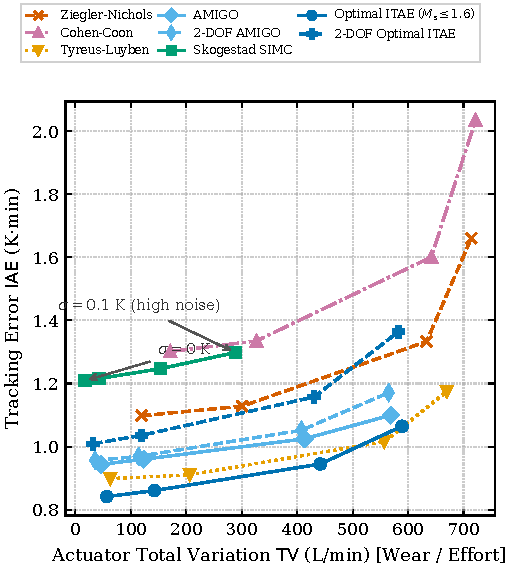
\includegraphics[width=0.55\textwidth]{figures/fig_noise_sensitivity.pdf}
    \caption{Mean true-temperature IAE versus mean valve travel as the sensor noise grows from $\sigma = 0$ to $0.1$~K, with the measurement filter $\tau_m = 0.05$~min ($30$ runs per point).}
    \label{fig:noise_sensitivity}
\end{figure}

{\renewcommand{\footnotesize}{\scriptsize}\begin{table*}[t]
\centering
\footnotesize
\caption{Sensitivity of tracking error (IAE) and actuator effort (TV) to measurement noise levels across $30$ Monte Carlo runs; $\tau_m$ is the time constant of the first-order measurement filter ($0$ = unfiltered).}
\label{tab:noise_sensitivity}
\resizebox{\ifdim\width>\textwidth\textwidth\else\width\fi}{!}{%
\begin{tabular}{lcccc}
\toprule
Method & $\tau_m$ (min) & Noise $\sigma$ (K) & IAE (mean $\pm$ std) & TV (L/min) \\
\midrule
Ziegler-Nichols & 0.00 & 0.0 & 0.94 $\pm$ 0.00 & 81.9 $\pm$ 0.0 \\
Ziegler-Nichols & 0.00 & 0.01 & 1.00 $\pm$ 0.02 & 585.3 $\pm$ 11.4 \\
Ziegler-Nichols & 0.00 & 0.05 & 1.43 $\pm$ 0.08 & 748.9 $\pm$ 5.6 \\
Ziegler-Nichols & 0.00 & 0.1 & 2.03 $\pm$ 0.18 & 773.7 $\pm$ 4.6 \\
Ziegler-Nichols & 0.05 & 0.0 & 1.10 $\pm$ 0.00 & 119.5 $\pm$ 0.0 \\
Ziegler-Nichols & 0.05 & 0.01 & 1.13 $\pm$ 0.01 & 300.6 $\pm$ 5.5 \\
Ziegler-Nichols & 0.05 & 0.05 & 1.33 $\pm$ 0.08 & 633.5 $\pm$ 9.7 \\
Ziegler-Nichols & 0.05 & 0.1 & 1.66 $\pm$ 0.10 & 714.0 $\pm$ 9.0 \\
Cohen-Coon & 0.00 & 0.0 & 1.02 $\pm$ 0.00 & 104.0 $\pm$ 0.0 \\
Cohen-Coon & 0.00 & 0.01 & 1.08 $\pm$ 0.03 & 583.4 $\pm$ 12.4 \\
Cohen-Coon & 0.00 & 0.05 & 1.54 $\pm$ 0.11 & 749.3 $\pm$ 4.4 \\
Cohen-Coon & 0.00 & 0.1 & 2.12 $\pm$ 0.15 & 773.1 $\pm$ 4.4 \\
Cohen-Coon & 0.05 & 0.0 & 1.30 $\pm$ 0.00 & 171.0 $\pm$ 0.0 \\
Cohen-Coon & 0.05 & 0.01 & 1.34 $\pm$ 0.01 & 326.3 $\pm$ 5.2 \\
Cohen-Coon & 0.05 & 0.05 & 1.60 $\pm$ 0.08 & 641.8 $\pm$ 10.7 \\
Cohen-Coon & 0.05 & 0.1 & 2.04 $\pm$ 0.15 & 721.8 $\pm$ 7.3 \\
Tyreus-Luyben & 0.00 & 0.0 & 0.92 $\pm$ 0.00 & 48.8 $\pm$ 0.0 \\
Tyreus-Luyben & 0.00 & 0.01 & 0.96 $\pm$ 0.01 & 511.3 $\pm$ 11.9 \\
Tyreus-Luyben & 0.00 & 0.05 & 1.21 $\pm$ 0.04 & 722.5 $\pm$ 7.3 \\
Tyreus-Luyben & 0.00 & 0.1 & 1.51 $\pm$ 0.07 & 759.4 $\pm$ 7.5 \\
Tyreus-Luyben & 0.05 & 0.0 & 0.90 $\pm$ 0.00 & 62.9 $\pm$ 0.0 \\
Tyreus-Luyben & 0.05 & 0.01 & 0.91 $\pm$ 0.01 & 206.3 $\pm$ 4.2 \\
Tyreus-Luyben & 0.05 & 0.05 & 1.02 $\pm$ 0.03 & 557.2 $\pm$ 11.5 \\
Tyreus-Luyben & 0.05 & 0.1 & 1.17 $\pm$ 0.05 & 669.7 $\pm$ 8.1 \\
AMIGO & 0.00 & 0.0 & 0.93 $\pm$ 0.00 & 40.4 $\pm$ 0.0 \\
AMIGO & 0.00 & 0.01 & 0.94 $\pm$ 0.01 & 372.3 $\pm$ 10.5 \\
AMIGO & 0.00 & 0.05 & 1.05 $\pm$ 0.03 & 666.5 $\pm$ 9.1 \\
AMIGO & 0.00 & 0.1 & 1.24 $\pm$ 0.05 & 727.0 $\pm$ 7.7 \\
AMIGO & 0.05 & 0.0 & 0.94 $\pm$ 0.00 & 45.9 $\pm$ 0.0 \\
AMIGO & 0.05 & 0.01 & 0.96 $\pm$ 0.00 & 123.3 $\pm$ 2.4 \\
AMIGO & 0.05 & 0.05 & 1.02 $\pm$ 0.02 & 413.4 $\pm$ 9.0 \\
AMIGO & 0.05 & 0.1 & 1.10 $\pm$ 0.04 & 568.9 $\pm$ 10.7 \\
2-DOF AMIGO & 0.00 & 0.0 & 0.96 $\pm$ 0.00 & 29.3 $\pm$ 0.0 \\
2-DOF AMIGO & 0.00 & 0.01 & 1.00 $\pm$ 0.02 & 366.7 $\pm$ 10.6 \\
2-DOF AMIGO & 0.00 & 0.05 & 1.26 $\pm$ 0.05 & 664.4 $\pm$ 9.7 \\
2-DOF AMIGO & 0.00 & 0.1 & 1.53 $\pm$ 0.07 & 725.8 $\pm$ 7.3 \\
2-DOF AMIGO & 0.05 & 0.0 & 0.96 $\pm$ 0.00 & 35.5 $\pm$ 0.0 \\
2-DOF AMIGO & 0.05 & 0.01 & 0.97 $\pm$ 0.01 & 113.9 $\pm$ 2.6 \\
2-DOF AMIGO & 0.05 & 0.05 & 1.05 $\pm$ 0.02 & 407.7 $\pm$ 9.1 \\
2-DOF AMIGO & 0.05 & 0.1 & 1.17 $\pm$ 0.04 & 565.1 $\pm$ 10.8 \\
Skogestad SIMC & 0.00 & 0.0 & 1.29 $\pm$ 0.00 & 15.7 $\pm$ 0.0 \\
Skogestad SIMC & 0.00 & 0.01 & 1.29 $\pm$ 0.00 & 133.2 $\pm$ 4.5 \\
Skogestad SIMC & 0.00 & 0.05 & 1.44 $\pm$ 0.05 & 474.1 $\pm$ 12.0 \\
Skogestad SIMC & 0.00 & 0.1 & 1.71 $\pm$ 0.07 & 603.0 $\pm$ 11.4 \\
Skogestad SIMC & 0.05 & 0.0 & 1.21 $\pm$ 0.00 & 17.2 $\pm$ 0.0 \\
Skogestad SIMC & 0.05 & 0.01 & 1.22 $\pm$ 0.00 & 42.7 $\pm$ 0.8 \\
Skogestad SIMC & 0.05 & 0.05 & 1.25 $\pm$ 0.01 & 153.0 $\pm$ 4.1 \\
Skogestad SIMC & 0.05 & 0.1 & 1.30 $\pm$ 0.02 & 288.3 $\pm$ 7.6 \\
Optimal ITAE ($M_s \leq 1.6$) & 0.00 & 0.0 & 0.83 $\pm$ 0.00 & 48.6 $\pm$ 0.0 \\
Optimal ITAE ($M_s \leq 1.6$) & 0.00 & 0.01 & 0.85 $\pm$ 0.00 & 400.6 $\pm$ 11.2 \\
Optimal ITAE ($M_s \leq 1.6$) & 0.00 & 0.05 & 1.03 $\pm$ 0.03 & 677.9 $\pm$ 9.7 \\
Optimal ITAE ($M_s \leq 1.6$) & 0.00 & 0.1 & 1.27 $\pm$ 0.05 & 734.1 $\pm$ 6.8 \\
Optimal ITAE ($M_s \leq 1.6$) & 0.05 & 0.0 & 0.84 $\pm$ 0.00 & 56.6 $\pm$ 0.0 \\
Optimal ITAE ($M_s \leq 1.6$) & 0.05 & 0.01 & 0.86 $\pm$ 0.00 & 142.3 $\pm$ 2.7 \\
Optimal ITAE ($M_s \leq 1.6$) & 0.05 & 0.05 & 0.94 $\pm$ 0.02 & 441.8 $\pm$ 10.1 \\
Optimal ITAE ($M_s \leq 1.6$) & 0.05 & 0.1 & 1.06 $\pm$ 0.03 & 589.2 $\pm$ 11.0 \\
2-DOF Optimal ITAE & 0.00 & 0.0 & 1.08 $\pm$ 0.00 & 25.0 $\pm$ 0.0 \\
2-DOF Optimal ITAE & 0.00 & 0.01 & 1.13 $\pm$ 0.02 & 389.7 $\pm$ 10.9 \\
2-DOF Optimal ITAE & 0.00 & 0.05 & 1.50 $\pm$ 0.05 & 675.0 $\pm$ 8.9 \\
2-DOF Optimal ITAE & 0.00 & 0.1 & 1.80 $\pm$ 0.07 & 732.5 $\pm$ 6.7 \\
2-DOF Optimal ITAE & 0.05 & 0.0 & 1.01 $\pm$ 0.00 & 31.3 $\pm$ 0.0 \\
2-DOF Optimal ITAE & 0.05 & 0.01 & 1.04 $\pm$ 0.02 & 119.4 $\pm$ 2.7 \\
2-DOF Optimal ITAE & 0.05 & 0.05 & 1.16 $\pm$ 0.04 & 430.3 $\pm$ 9.5 \\
2-DOF Optimal ITAE & 0.05 & 0.1 & 1.36 $\pm$ 0.05 & 582.8 $\pm$ 10.5 \\
\bottomrule
\end{tabular}%
}
\end{table*}
}

\begin{table*}[t]
\centering
\footnotesize
\caption{Effect of the measurement filter ($\tau_m = 0.05$~min against none) on the $30$ paired noise realizations: mean paired difference and Wilcoxon signed-rank $p$-values adjusted by Benjamini--Hochberg over all tests in the table.}
\label{tab:noise_filter_paired}
\resizebox{\ifdim\width>\textwidth\textwidth\else\width\fi}{!}{%
\begin{tabular}{lccccc}
\toprule
Method & Noise $\sigma$ (K) & \(\Delta\)TV (L/min) & \(p_{\mathrm{adj}}\) (TV) & \(\Delta\)IAE (K$\cdot$min) & \(p_{\mathrm{adj}}\) (IAE) \\
\midrule
Ziegler-Nichols & 0.01 & -284.8 & $<10^{-3}$ & +0.127 & $<10^{-3}$ \\
Ziegler-Nichols & 0.05 & -115.4 & $<10^{-3}$ & -0.100 & $<10^{-3}$ \\
Ziegler-Nichols & 0.10 & -59.7 & $<10^{-3}$ & -0.370 & $<10^{-3}$ \\
Cohen-Coon & 0.01 & -257.1 & $<10^{-3}$ & +0.255 & $<10^{-3}$ \\
Cohen-Coon & 0.05 & -107.5 & $<10^{-3}$ & +0.059 & 0.020 \\
Cohen-Coon & 0.10 & -51.3 & $<10^{-3}$ & -0.085 & 0.040 \\
Tyreus-Luyben & 0.01 & -305.0 & $<10^{-3}$ & -0.046 & $<10^{-3}$ \\
Tyreus-Luyben & 0.05 & -165.3 & $<10^{-3}$ & -0.192 & $<10^{-3}$ \\
Tyreus-Luyben & 0.10 & -89.7 & $<10^{-3}$ & -0.334 & $<10^{-3}$ \\
AMIGO & 0.01 & -249.0 & $<10^{-3}$ & +0.016 & $<10^{-3}$ \\
AMIGO & 0.05 & -253.2 & $<10^{-3}$ & -0.023 & $<10^{-3}$ \\
AMIGO & 0.10 & -158.0 & $<10^{-3}$ & -0.136 & $<10^{-3}$ \\
2-DOF AMIGO & 0.01 & -252.8 & $<10^{-3}$ & -0.033 & $<10^{-3}$ \\
2-DOF AMIGO & 0.05 & -256.8 & $<10^{-3}$ & -0.213 & $<10^{-3}$ \\
2-DOF AMIGO & 0.10 & -160.6 & $<10^{-3}$ & -0.357 & $<10^{-3}$ \\
Skogestad SIMC & 0.01 & -90.5 & $<10^{-3}$ & -0.078 & $<10^{-3}$ \\
Skogestad SIMC & 0.05 & -321.1 & $<10^{-3}$ & -0.194 & $<10^{-3}$ \\
Skogestad SIMC & 0.10 & -314.7 & $<10^{-3}$ & -0.410 & $<10^{-3}$ \\
Optimal ITAE ($M_s \leq 1.6$) & 0.01 & -258.3 & $<10^{-3}$ & +0.012 & $<10^{-3}$ \\
Optimal ITAE ($M_s \leq 1.6$) & 0.05 & -236.1 & $<10^{-3}$ & -0.080 & $<10^{-3}$ \\
Optimal ITAE ($M_s \leq 1.6$) & 0.10 & -144.8 & $<10^{-3}$ & -0.210 & $<10^{-3}$ \\
2-DOF Optimal ITAE & 0.01 & -270.3 & $<10^{-3}$ & -0.090 & $<10^{-3}$ \\
2-DOF Optimal ITAE & 0.05 & -244.7 & $<10^{-3}$ & -0.341 & $<10^{-3}$ \\
2-DOF Optimal ITAE & 0.10 & -149.7 & $<10^{-3}$ & -0.433 & $<10^{-3}$ \\
\bottomrule
\end{tabular}%
}
\end{table*}


Since the IAE is evaluated on the true temperature, the table measures how much sensor noise each loop converts into real thermal deviation. Without the filter, valve travel is bounded by $|u_0 - \bar q_j| + S_{\max}t_f \approx 800$~L/min and approaches this ceiling quickly: at $\sigma = 0.01$~K the travel is already $585.3$ (ZN), $583.4$ (CC) and $511.3$~L/min (TL), and at $0.1$~K every tuning except SIMC ($603.0$~L/min) lies between $725.8$ and $773.7$~L/min, which hides differences in valve wear. The ordering follows the high-frequency gain $|K_p|(1+N)$ of Table~\ref{tab:testbed}: ZN and CC, with $K_{\mathrm{hf}}$ of $490$ and $559$~L/min/K, are the noisiest, SIMC ($77$~L/min/K) the quietest.

The filter spreads the tunings out. At $\sigma = 0.01$~K the travel falls by a factor of $1.8$ to $3.3$ (ZN $585.3 \rightarrow 300.6$, TL $511.3 \rightarrow 206.3$, AMIGO $372.3 \rightarrow 123.3$, Optimal ITAE $400.6 \rightarrow 142.3$, SIMC $133.2 \rightarrow 42.7$~L/min), and the ratio between the noisiest and the quietest tuning grows from $4.4$ to $7.6$. At $\sigma = 0.05$~K the range is $153.0$ (SIMC) to $641.8$~L/min (CC). The filter is not sufficient for the empirical rules at $\sigma = 0.1$~K, where ZN and CC still reach $714.0$ and $721.8$~L/min, within $11\%$ of the ceiling, against $288.3$ for SIMC; a lower $N$ or a larger $\tau_m$ is needed there. All $24$ paired travel differences are significant after Benjamini--Hochberg adjustment ($p_{\mathrm{adj}} < 10^{-3}$), but with effects of $51$ to $321$~L/min against intervals of a few L/min the $p$-values carry no information; the relevant quantity is the size of the effect, a reduction of $7\%$ (CC, $\sigma = 0.1$~K) to $69\%$ (2-DOF AMIGO and 2-DOF Optimal ITAE, $\sigma = 0.01$~K) of the unfiltered travel (Table~\ref{tab:noise_filter_paired}). The effect on the tracking error depends on the noise level: at $\sigma = 0.01$~K the filter \emph{increases} the IAE of ZN ($+0.127$~K$\cdot$min) and CC ($+0.255$), consistent with phase lag outweighing the small noise reduction, and marginally that of AMIGO ($+0.016$) and Optimal ITAE ($+0.012$); at $\sigma \ge 0.05$~K it lowers the IAE of every tuning except CC at $0.05$~K ($+0.059$). The cost is the phase lag of the filter in the noise-free loop (IAE $0.94 \rightarrow 1.10$ for ZN and $1.02 \rightarrow 1.30$~K$\cdot$min for CC, but $0.83 \rightarrow 0.84$ for Optimal ITAE and $1.29 \rightarrow 1.21$ for SIMC). With the filter at $\sigma = 0.1$~K the true-temperature error ranks Optimal ITAE ($1.06 \pm 0.01$~K$\cdot$min), AMIGO ($1.10 \pm 0.01$), TL ($1.17 \pm 0.02$) and SIMC ($1.30 \pm 0.01$) ahead of ZN ($1.66 \pm 0.04$) and CC ($2.04 \pm 0.06$), with non-overlapping $95\%$ intervals.

\paragraph{The derivative-filter coefficient as a design variable.} The high-frequency gain $K_{\mathrm{hf}} = |K_p|(1+N)$ depends on $N$ as much as on the tuning rule, and the benchmark uses $N = 10$ for every rule. Table~\ref{tab:n_design} lowers $N$ for ZN and CC: $N = 3$ cuts $K_{\mathrm{hf}}$ by $64\%$ ($490 \rightarrow 178$ and $559 \rightarrow 203$~L/min/K) without changing the noise-free IAE ($0.940 \rightarrow 0.942$ and $1.017 \rightarrow 1.010$~K$\cdot$min), and at $\sigma = 0.01$~K it reduces the travel from $585$ to $529$~L/min (ZN) and from $583$ to $543$ (CC), i.e.\ $10\%$ and $7\%$. At $\sigma = 0.05$~K the travel stays between $731$ and $749$~L/min, near the $800$~L/min ceiling, for every $N$. A smaller $N$ is thus a free reduction of noise gain for these rules, but it is a weaker remedy than the measurement filter ($-49\%$ and $-44\%$ at $\sigma = 0.01$~K), and it does not remove the discrimination problem of TV at large noise.

\begin{table*}[t]
\centering
\footnotesize
\caption{Derivative-filter coefficient $N$ ($\tau_f = T_d/N$) as a design variable for the empirical rules, $-2$~K step, unfiltered measurement; $K_{\mathrm{hf}} = |K_p|(1+N)$ equals $\|CS\|_\infty$ to within $0.3$~L/min/K in every row. Noise columns: mean $\pm$ $95\%$ half-width over 30 realizations; TV in L/min, IAE in K$\cdot$min.}
\label{tab:n_design}
\resizebox{\ifdim\width>\textwidth\textwidth\else\width\fi}{!}{%
\begin{tabular}{lcccccccc}
\toprule
Method & \(N\) & \(K_{\mathrm{hf}}\) (L/min/K) & IAE (noise-free) & \(M_p\) (\%) & IAE ($\sigma=0.01$) & TV ($\sigma=0.01$) & IAE ($\sigma=0.05$) & TV ($\sigma=0.05$) \\
\midrule
Ziegler-Nichols & 3 & 178 & 0.942 & 23.3 & 0.99 $\pm$ 0.01 & 523 $\pm$ 4 & 1.27 $\pm$ 0.03 & 726 $\pm$ 3 \\
Ziegler-Nichols & 5 & 267 & 0.941 & 22.9 & 0.99 $\pm$ 0.01 & 553 $\pm$ 4 & 1.33 $\pm$ 0.03 & 736 $\pm$ 4 \\
Ziegler-Nichols & 10 & 490 & 0.940 & 22.6 & 1.00 $\pm$ 0.01 & 581 $\pm$ 4 & 1.39 $\pm$ 0.03 & 743 $\pm$ 3 \\
Cohen-Coon & 3 & 203 & 1.010 & 31.4 & 1.07 $\pm$ 0.01 & 537 $\pm$ 4 & 1.43 $\pm$ 0.04 & 732 $\pm$ 3 \\
Cohen-Coon & 5 & 305 & 1.011 & 31.1 & 1.07 $\pm$ 0.01 & 558 $\pm$ 4 & 1.46 $\pm$ 0.03 & 738 $\pm$ 3 \\
Cohen-Coon & 10 & 559 & 1.017 & 31.0 & 1.08 $\pm$ 0.01 & 578 $\pm$ 4 & 1.50 $\pm$ 0.04 & 744 $\pm$ 3 \\
\bottomrule
\end{tabular}%
}
\end{table*}


\paragraph{Integrator policies under noise.} Table~\ref{tab:noise_policies} repeats the nominal step for no anti-windup, back-calculation with the noise-free $T_t^{\mathrm{cv}}$ and the directional rule with $30$ noise realizations. At $\sigma = 0.01$~K the ratio of back-calculation to the rule stays between $\vnzbclomin$ and $\vnzbclomax$; at $0.05$~K back-calculation is up to $\vnzbchimaxpct\%$ worse for \vnzbcworse{} and better for \vnzbcbetter{}. The valve travel is set by the noise and is almost the same for the three policies. No anti-windup remains at least $\vnzempnonemin$ times worse for ZN and CC, and the directional rule still worsens SIMC ($\vnzSIMCdir$ against $\vnzSIMCnone$ at $0.05$~K). A tracking constant chosen with noise was not tried.

\begin{table*}[t]
\centering
\footnotesize
\caption{Integrator policies under Gaussian sensor noise, $-2$~K step, unfiltered measurement, 30 realizations per level (seeds of the noise campaign): IAE on the true temperature (K$\cdot$min, mean $\pm$ half-width of the $95\%$ $t$-interval) and mean TV (L/min). BC uses the $T_t^{\mathrm{sel}}$ of Table~\ref{tab:antiwindup_tt_summary}; ``Directional'' is Eq.~\eqref{eq:clamping_antiwindup}.}
\label{tab:noise_policies}
\resizebox{\ifdim\width>\textwidth\textwidth\else\width\fi}{!}{%
\begin{tabular}{lccccccc}
\toprule
Method & \(\sigma\) (K) & IAE None & TV None & IAE BC ($T_t^{\mathrm{sel}}$) & TV BC ($T_t^{\mathrm{sel}}$) & IAE Directional & TV Directional \\
\midrule
Ziegler-Nichols & 0 & 91.11 & 767 & 0.88 & 71 & 0.94 & 82 \\
Ziegler-Nichols & 0.01 & 91.17 $\pm$ 0.08 & 768 & 1.09 $\pm$ 0.01 & 591 & 1.00 $\pm$ 0.01 & 585 \\
Ziegler-Nichols & 0.05 & 91.06 $\pm$ 0.09 & 769 & 2.16 $\pm$ 0.07 & 749 & 1.43 $\pm$ 0.03 & 749 \\
Cohen-Coon & 0 & 87.37 & 778 & 0.82 & 62 & 1.02 & 104 \\
Cohen-Coon & 0.01 & 87.37 $\pm$ 0.00 & 778 & 1.06 $\pm$ 0.01 & 585 & 1.08 $\pm$ 0.01 & 583 \\
Cohen-Coon & 0.05 & 87.90 $\pm$ 0.35 & 777 & 2.24 $\pm$ 0.07 & 749 & 1.54 $\pm$ 0.04 & 749 \\
Tyreus-Luyben & 0 & 1.26 & 82 & 0.83 & 52 & 0.92 & 49 \\
Tyreus-Luyben & 0.01 & 1.28 $\pm$ 0.00 & 522 & 0.86 $\pm$ 0.00 & 513 & 0.96 $\pm$ 0.00 & 511 \\
Tyreus-Luyben & 0.05 & 1.46 $\pm$ 0.01 & 725 & 1.11 $\pm$ 0.01 & 722 & 1.21 $\pm$ 0.02 & 723 \\
AMIGO & 0 & 1.60 & 108 & 0.92 & 37 & 0.93 & 40 \\
AMIGO & 0.01 & 1.62 $\pm$ 0.01 & 409 & 0.95 $\pm$ 0.00 & 371 & 0.94 $\pm$ 0.00 & 372 \\
AMIGO & 0.05 & 1.89 $\pm$ 0.03 & 677 & 1.36 $\pm$ 0.03 & 668 & 1.05 $\pm$ 0.01 & 667 \\
Skogestad SIMC & 0 & 1.09 & 22 & 1.15 & 19 & 1.29 & 16 \\
Skogestad SIMC & 0.01 & 1.09 $\pm$ 0.00 & 137 & 1.16 $\pm$ 0.00 & 135 & 1.29 $\pm$ 0.00 & 133 \\
Skogestad SIMC & 0.05 & 1.13 $\pm$ 0.01 & 475 & 1.22 $\pm$ 0.01 & 475 & 1.44 $\pm$ 0.02 & 474 \\
Optimal ITAE ($M_s^{\mathrm{FOPTD}} \leq 1.6$) & 0 & 1.51 & 112 & 0.83 & 50 & 0.83 & 49 \\
Optimal ITAE ($M_s^{\mathrm{FOPTD}} \leq 1.6$) & 0.01 & 1.54 $\pm$ 0.01 & 436 & 0.86 $\pm$ 0.00 & 402 & 0.85 $\pm$ 0.00 & 401 \\
Optimal ITAE ($M_s^{\mathrm{FOPTD}} \leq 1.6$) & 0.05 & 1.76 $\pm$ 0.03 & 689 & 1.09 $\pm$ 0.01 & 678 & 1.03 $\pm$ 0.01 & 678 \\
\bottomrule
\end{tabular}%
}
\end{table*}


\paragraph{Tracking constant under noise and mechanism.} Table~\ref{tab:noise_ttcv} re-chooses $T_t^{\mathrm{cv}}$ by the criterion of Table~\ref{tab:antiwindup_tt_summary} with $\sigma = 0.05$~K. The constant moves up for \vnzttchanged{} and stays for the other loops; with the new constant the worst ratio of back-calculation to the directional rule on $-2$~K falls from $\vnzttbeforemax$ to $\vnzttaftermax$ and on $\pm 5$~K is at most $\vnzttfiveaftermax$, so the gap narrows but does not close. Table~\ref{tab:noise_mechanism} tests the mechanism: the share of samples in which a limit cuts the command is the same under both rules, so noise does not make back-calculation saturate more often; what differs is what the integrator does with each cut. The directional rule freezes it, whereas back-calculation with a small $T_t$ adds $(\Delta t/T_t)(u_{\text{act},k-1} - u_{\text{raw},k-1})$ at every cut, $\vmechtrackmin$ to $\vmechtrackmax$~L/min per sample for ZN and CC, and its integrator departs from the noise-free path $\vmechrmsratiomin$ to $\vmechrmsratiomax$ times more.

\begin{table*}[t]
\centering
\footnotesize
\caption{Tracking constant re-chosen under sensor noise ($\sigma = 0.05$~K, 30 realizations, seeds of the noise campaign, unfiltered measurement): $T_t^{\mathrm{sel,noise}}$ minimizes the mean IAE of the $-2$~K step inside $[T_d, T_i]$; IAE (K$\cdot$min, mean $\pm$ $95\%$ half-width) under the same noise for back-calculation with the noise-free and the noise-chosen constant and for the directional rule.}
\label{tab:noise_ttcv}
\resizebox{\ifdim\width>\textwidth\textwidth\else\width\fi}{!}{%
\begin{tabular}{lccccc}
\toprule
Method & \(T_t^{\mathrm{sel}}\), \(T_t^{\mathrm{sel,noise}}\) (min) & Step & IAE BC ($T_t^{\mathrm{sel}}$) & IAE BC ($T_t^{\mathrm{sel,noise}}$) & IAE Directional \\
\midrule
Ziegler-Nichols & 0.047, 0.093 & $-2$ K & 2.16 $\pm$ 0.07 & 1.84 $\pm$ 0.05 & 1.43 $\pm$ 0.03 \\
 &  & $-5$ K & 4.74 $\pm$ 0.09 & 4.53 $\pm$ 0.05 & 3.82 $\pm$ 0.03 \\
 &  & $+5$ K & 4.61 $\pm$ 0.11 & 4.64 $\pm$ 0.09 & 4.39 $\pm$ 0.08 \\
Cohen-Coon & 0.033, 0.089 & $-2$ K & 2.24 $\pm$ 0.07 & 1.63 $\pm$ 0.04 & 1.54 $\pm$ 0.04 \\
 &  & $-5$ K & 4.74 $\pm$ 0.09 & 4.16 $\pm$ 0.05 & 3.98 $\pm$ 0.03 \\
 &  & $+5$ K & 4.64 $\pm$ 0.10 & 4.08 $\pm$ 0.06 & 5.08 $\pm$ 0.10 \\
Tyreus-Luyben & 0.554, 0.554 & $-2$ K & 1.11 $\pm$ 0.01 & 1.11 $\pm$ 0.01 & 1.21 $\pm$ 0.02 \\
 &  & $-5$ K & 3.47 $\pm$ 0.01 & 3.47 $\pm$ 0.01 & 3.97 $\pm$ 0.02 \\
 &  & $+5$ K & 3.32 $\pm$ 0.02 & 3.32 $\pm$ 0.02 & 3.75 $\pm$ 0.04 \\
AMIGO & 0.121, 0.247 & $-2$ K & 1.36 $\pm$ 0.03 & 1.25 $\pm$ 0.02 & 1.05 $\pm$ 0.01 \\
 &  & $-5$ K & 3.77 $\pm$ 0.03 & 3.71 $\pm$ 0.02 & 3.42 $\pm$ 0.01 \\
 &  & $+5$ K & 3.40 $\pm$ 0.04 & 3.49 $\pm$ 0.03 & 3.05 $\pm$ 0.01 \\
Skogestad SIMC & 0.643, 0.643 & $-2$ K & 1.22 $\pm$ 0.01 & 1.22 $\pm$ 0.01 & 1.44 $\pm$ 0.02 \\
 &  & $-5$ K & 3.84 $\pm$ 0.01 & 3.84 $\pm$ 0.01 & 4.80 $\pm$ 0.04 \\
 &  & $+5$ K & 3.23 $\pm$ 0.01 & 3.23 $\pm$ 0.01 & 3.92 $\pm$ 0.03 \\
Optimal ITAE ($M_s^{\mathrm{FOPTD}} \leq 1.6$) & 0.300, 0.300 & $-2$ K & 1.09 $\pm$ 0.01 & 1.09 $\pm$ 0.01 & 1.03 $\pm$ 0.01 \\
 &  & $-5$ K & 3.39 $\pm$ 0.01 & 3.39 $\pm$ 0.01 & 3.50 $\pm$ 0.01 \\
 &  & $+5$ K & 3.24 $\pm$ 0.02 & 3.24 $\pm$ 0.02 & 3.38 $\pm$ 0.04 \\
\bottomrule
\end{tabular}%
}
\end{table*}


\begin{table*}[t]
\centering
\footnotesize
\caption{Mechanism under sensor noise ($\sigma = 0.05$~K, $-2$~K step, 30 realizations): share of samples in which a limit cuts the command ($u_{\text{act}} \ne u_{\text{raw}}$), RMS deviation (L/min) of the integrator from its noise-free trajectory, and mean magnitude of the back-calculation increment $(\Delta t/T_t)|u_{\text{act},k-1} - u_{\text{raw},k-1}|$ with $T_t^{\mathrm{cv}}$.}
\label{tab:noise_mechanism}
\resizebox{\ifdim\width>\textwidth\textwidth\else\width\fi}{!}{%
\begin{tabular}{lccccc}
\toprule
Method & cut share BC ($T_t^{\mathrm{cv}}$) & RMS \(I - I_0\) BC ($T_t^{\mathrm{cv}}$) & mean tracking step (L/min) & cut share Directional & RMS \(I - I_0\) Directional \\
\midrule
Ziegler-Nichols & 0.87 & 7.7 & 2.90 & 0.87 & 1.5 \\
Cohen-Coon & 0.87 & 9.6 & 4.01 & 0.87 & 1.3 \\
Tyreus-Luyben & 0.80 & 0.5 & 0.16 & 0.80 & 1.0 \\
AMIGO & 0.67 & 1.2 & 0.32 & 0.66 & 0.7 \\
Skogestad SIMC & 0.26 & 0.1 & 0.01 & 0.26 & 0.3 \\
Optimal ITAE ($M_s^{\mathrm{FOPTD}} \leq 1.6$) & 0.69 & 0.5 & 0.17 & 0.69 & 0.6 \\
\bottomrule
\end{tabular}%
}
\end{table*}


\paragraph{Steps of both signs and the measurement filter.} Table~\ref{tab:noise_policies_ext} repeats Table~\ref{tab:noise_policies} on the $\pm 5$~K steps and with the filter $\tau_m = 0.05$~min. Without the filter, at $\sigma = 0.05$~K, back-calculation with the noise-free $T_t^{\mathrm{cv}}$ is up to $\vextrawmax$ times the IAE of the directional rule; with the filter the worst ratio over steps, noise levels and loops is $\vextfiltmax$. No anti-windup remains at least $\vextempnonemin$ times worse than the directional rule for ZN and CC in every combination.

\begin{table*}[t]
\centering
\footnotesize
\caption{Table~\ref{tab:noise_policies} extended to the $\pm 5$~K steps and to the filtered measurement ($\tau_m = 0.05$~min), 30 realizations: each cell is $\mathrm{IAE}_{\mathrm{BC}}/\mathrm{IAE}_{\mathrm{dir}}$ / $\mathrm{IAE}_{\mathrm{none}}/\mathrm{IAE}_{\mathrm{dir}}$ (means over seeds; BC with the noise-free $T_t^{\mathrm{cv}}$). Means and intervals are in \texttt{results/jpc/noise\_policies\_ext\_full.csv}.}
\label{tab:noise_policies_ext}
\resizebox{\ifdim\width>\textwidth\textwidth\else\width\fi}{!}{%
\begin{tabular}{lccccc}
\toprule
Method & Step & $\sigma=0.01$, $\tau_m=0$ & $\sigma=0.05$, $\tau_m=0$ & $\sigma=0.01$, $\tau_m=0.05$ & $\sigma=0.05$, $\tau_m=0.05$ \\
\midrule
Ziegler-Nichols & $-2$ K & 1.09 / 91.04 & 1.50 / 63.52 & 1.01 / 71.25 & 1.15 / 59.76 \\
 & $-5$ K & 1.08 / 24.03 & 1.24 / 21.25 & 1.04 / 23.37 & 1.11 / 22.64 \\
 & $+5$ K & 0.90 / 32.32 & 1.05 / 27.62 & 0.82 / 28.77 & 0.87 / 27.27 \\
Cohen-Coon & $-2$ K & 0.98 / 80.92 & 1.45 / 57.01 & 0.77 / 63.09 & 0.88 / 52.58 \\
 & $-5$ K & 0.99 / 22.37 & 1.19 / 19.72 & 0.91 / 21.52 & 0.96 / 20.52 \\
 & $+5$ K & 0.71 / 26.27 & 0.91 / 22.80 & 0.52 / 19.98 & 0.55 / 18.87 \\
Tyreus-Luyben & $-2$ K & 0.90 / 1.34 & 0.92 / 1.21 & 0.94 / 1.49 & 0.94 / 1.42 \\
 & $-5$ K & 0.92 / 1.51 & 0.87 / 1.44 & 0.93 / 1.83 & 0.91 / 1.78 \\
 & $+5$ K & 0.91 / 2.28 & 0.88 / 2.19 & 0.91 / 4.58 & 0.90 / 4.39 \\
AMIGO & $-2$ K & 1.01 / 1.71 & 1.30 / 1.80 & 0.99 / 2.29 & 1.02 / 2.28 \\
 & $-5$ K & 1.00 / 12.34 & 1.11 / 11.98 & 1.00 / 15.26 & 1.01 / 14.99 \\
 & $+5$ K & 1.01 / 30.55 & 1.12 / 29.29 & 1.00 / 33.74 & 1.01 / 32.71 \\
Skogestad SIMC & $-2$ K & 0.90 / 0.85 & 0.84 / 0.79 & 0.91 / 0.88 & 0.91 / 0.88 \\
 & $-5$ K & 0.86 / 0.86 & 0.80 / 0.79 & 0.85 / 0.90 & 0.86 / 0.91 \\
 & $+5$ K & 0.86 / 0.97 & 0.82 / 0.93 & 0.88 / 1.06 & 0.87 / 1.05 \\
Optimal ITAE ($M_s^{\mathrm{FOPTD}} \leq 1.6$) & $-2$ K & 1.01 / 1.81 & 1.07 / 1.72 & 1.02 / 2.66 & 1.03 / 2.51 \\
 & $-5$ K & 0.97 / 4.26 & 0.97 / 4.05 & 1.00 / 10.00 & 0.99 / 9.64 \\
 & $+5$ K & 0.98 / 23.55 & 0.96 / 21.28 & 0.97 / 24.57 & 0.97 / 23.80 \\
\bottomrule
\end{tabular}%
}
\end{table*}


\paragraph{Rate demand under noise.} Table~\ref{tab:rho_noise} recomputes $\rho$ and $R$ under noise. On the raw measurement at $\sigma = 0.05$~K the largest command increment is set by the noise, $\rho$ of SIMC reaches $\vrhonzrawSIMCmax$ and $\vrhonzrawwrong$ of the $\vrhonzcases$ cases have $\rho \ge 1$ with $R < 1$; with the measurement filter the SIMC demand stays at most $\vrhonzfiltSIMCmax$ and no case is misclassified, as without noise. In practice $\rho$ should be computed on the filtered loop or from a noise-free model run.

\begin{table*}[t]
\centering
\footnotesize
\caption{Rate demand under sensor noise, $S_{\max} = 80$~L/min$^2$, 30 realizations: each cell is $\rho$ / $R = \mathrm{IAE}_{\mathrm{amp}}/\mathrm{IAE}_{\mathrm{rate}}$ (means over seeds), with the raw ($\tau_m = 0$) or filtered ($\tau_m = 0.05$~min) measurement; $\rho$ is computed from the command of the same loop with the slew limit removed, as in Table~\ref{tab:rate_demand}.}
\label{tab:rho_noise}
\resizebox{\ifdim\width>\textwidth\textwidth\else\width\fi}{!}{%
\begin{tabular}{lcccccc}
\toprule
Method & Step & noise-free & $\sigma=0.01$, $\tau_m=0$ & $\sigma=0.01$, $\tau_m=0.05$ & $\sigma=0.05$, $\tau_m=0$ & $\sigma=0.05$, $\tau_m=0.05$ \\
\midrule
Ziegler-Nichols & $-2$ K & 5.11 / 23.52 & 7.21 / 22.20 & 7.41 / 22.12 & 23.43 / 15.32 & 9.46 / 18.69 \\
 & $-5$ K & 15.36 / 6.75 & 13.95 / 6.51 & 9.76 / 6.66 & 24.00 / 5.64 & 11.54 / 6.43 \\
 & $+5$ K & 10.63 / 7.72 & 11.79 / 7.51 & 11.93 / 6.54 & 24.45 / 6.15 & 13.34 / 6.20 \\
Cohen-Coon & $-2$ K & 6.72 / 20.26 & 8.45 / 19.17 & 9.01 / 17.53 & 22.24 / 13.01 & 10.87 / 14.60 \\
 & $-5$ K & 11.03 / 6.07 & 11.10 / 5.96 & 10.91 / 5.92 & 22.40 / 5.18 & 13.24 / 5.66 \\
 & $+5$ K & 13.99 / 5.92 & 15.04 / 5.85 & 15.24 / 4.53 & 24.19 / 4.94 & 16.40 / 4.30 \\
Tyreus-Luyben & $-2$ K & 2.75 / 1.38 & 4.16 / 1.34 & 2.84 / 1.49 & 16.26 / 1.21 & 4.39 / 1.42 \\
 & $-5$ K & 5.89 / 1.55 & 7.01 / 1.51 & 5.31 / 1.83 & 16.47 / 1.44 & 6.68 / 1.78 \\
 & $+5$ K & 8.70 / 1.16 & 9.91 / 1.14 & 8.56 / 1.40 & 16.81 / 1.08 & 9.47 / 1.40 \\
AMIGO & $-2$ K & 0.83 / 1.73 & 1.92 / 1.71 & 1.25 / 2.29 & 9.05 / 1.81 & 2.31 / 2.28 \\
 & $-5$ K & 2.10 / 9.38 & 2.57 / 9.30 & 2.96 / 9.81 & 9.08 / 8.95 & 3.36 / 9.66 \\
 & $+5$ K & 3.73 / 10.29 & 4.38 / 10.20 & 4.51 / 12.42 & 9.38 / 9.24 & 5.16 / 12.04 \\
Skogestad SIMC & $-2$ K & 0.21 / 0.85 & 0.58 / 0.85 & 0.27 / 0.88 & 2.90 / 0.79 & 0.67 / 0.88 \\
 & $-5$ K & 0.52 / 0.86 & 0.64 / 0.86 & 0.63 / 0.90 & 2.90 / 0.79 & 0.80 / 0.91 \\
 & $+5$ K & 0.51 / 0.97 & 0.70 / 0.97 & 0.63 / 1.06 & 2.92 / 0.93 & 0.84 / 1.05 \\
Optimal ITAE ($M_s^{\mathrm{FOPTD}} \leq 1.6$) & $-2$ K & 1.55 / 1.82 & 2.51 / 1.81 & 1.96 / 2.66 & 9.90 / 1.72 & 2.91 / 2.51 \\
 & $-5$ K & 2.93 / 4.38 & 3.85 / 4.26 & 3.49 / 7.80 & 9.97 / 3.99 & 4.42 / 7.67 \\
 & $+5$ K & 5.37 / 4.53 & 5.91 / 4.61 & 6.12 / 7.96 & 10.58 / 4.15 & 6.81 / 7.62 \\
\bottomrule
\end{tabular}%
}
\end{table*}


\section{Load disturbances: replicated runs}\label{supp:load}
\subsection{Unmeasured load disturbances}
\label{supp:loadfull}
A feed temperature step $\Delta T_f = +2$~K at $t = 2$~min and a feed concentration step $\Delta C_{Af} = +0.1$~mol/L ($+10\%$) at $t = 8$~min were applied at constant setpoint. Table~\ref{tab:load_disturbance} is the deterministic response (no noise, no measurement filter) and ranks the loops without sampling uncertainty; Table~\ref{tab:load_replicated} repeats the run with $30$ independent noise realizations ($\sigma = 0.05$~K), without and with the measurement filter ($\tau_m = 0.05$~min), and reports mean $\pm$ the half-width of the $95\%$ $t$-interval (Fig.~\ref{fig:disturbance_rejection} shows the deterministic response).

\begin{figure*}[t]
    \centering
    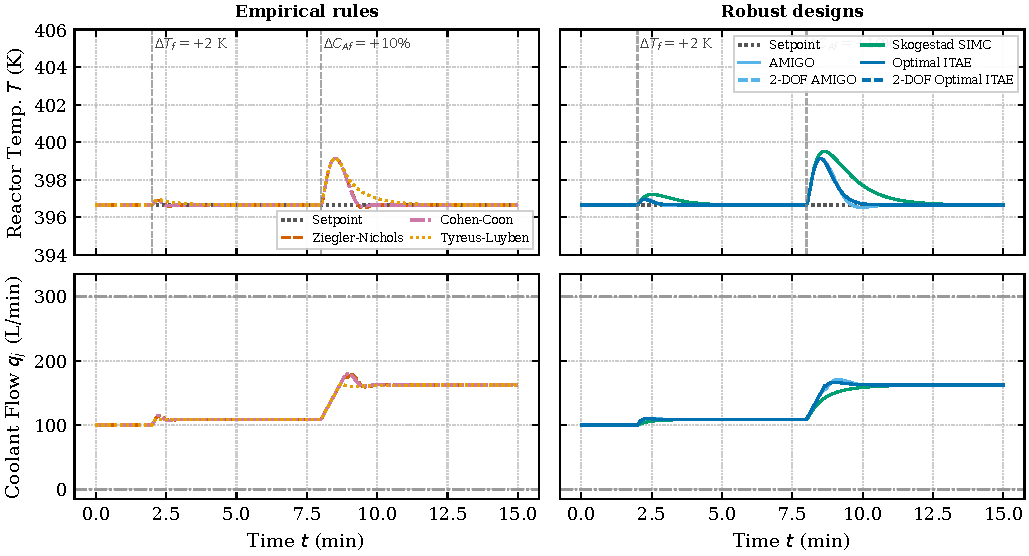
\includegraphics[width=0.92\textwidth]{figures/fig2_disturbance_rejection.pdf}
    \caption{Deterministic rejection of a $+2$~K feed temperature step at $t = 2$~min and a $+10\%$ feed concentration step at $t = 8$~min: empirical rules (left) and robust designs (right).}
    \label{fig:disturbance_rejection}
\end{figure*}

\begin{table*}[t]
\centering
\footnotesize
\caption{Regulatory performance under combined feed temperature ($+2$~K) and concentration ($+10\%$) load disturbances. $T(t_f) - T_{sp}$ is the true temperature error at $t_f = 15$~min.}
\label{tab:load_disturbance}
\resizebox{\ifdim\width>\textwidth\textwidth\else\width\fi}{!}{%
\begin{tabular}{lcccccc}
\toprule
Method & IAE & ITAE & TV (L/min) & Peak Dev (K) & Max Valve (L/min) & \(T(t_f) - T_{sp}\) (K) \\
\midrule
Ziegler-Nichols & 2.38 & 19.48 & 1116.7 & 2.51 & 177.9 & -0.07 \\
Cohen-Coon & 2.39 & 19.43 & 1117.0 & 2.49 & 178.2 & -0.06 \\
Tyreus-Luyben & 4.16 & 36.46 & 1077.6 & 2.54 & 166.2 & +0.02 \\
AMIGO & 3.01 & 24.64 & 991.1 & 2.53 & 167.5 & +0.01 \\
2-DOF AMIGO & 3.01 & 24.64 & 991.1 & 2.53 & 167.5 & +0.01 \\
Skogestad SIMC & 7.05 & 62.23 & 692.8 & 3.07 & 163.7 & +0.04 \\
Optimal ITAE ($M_s \leq 1.6$) & 3.23 & 27.04 & 1011.1 & 2.51 & 165.4 & +0.00 \\
2-DOF Optimal ITAE & 3.23 & 27.04 & 1011.1 & 2.51 & 165.4 & +0.00 \\
\bottomrule
\end{tabular}%
}
\end{table*}


\begin{table*}[t]
\centering
\footnotesize
\caption{Load profile of Section~\ref{subsec:load_results} with 30 independent noise realizations ($\sigma = 0.05$~K), without ($\tau_m = 0$) and with ($\tau_m = 0.05$~min) measurement filter: mean $\pm$ half-width of the $95\%$ $t$-interval. Errors are measured on the true temperature; the TV ceiling is $S_{\max}t_f = 1200$~L/min.}
\label{tab:load_replicated}
\resizebox{\ifdim\width>\textwidth\textwidth\else\width\fi}{!}{%
\begin{tabular}{lccccc}
\toprule
Method & \(\tau_m\) (min) & IAE & Peak dev. (K) & TV (L/min) & TV/ceiling (\%) \\
\midrule
Ziegler-Nichols & 0.00 & 2.59 $\pm$ 0.07 & 2.54 $\pm$ 0.06 & 1114 $\pm$ 4 & 93 \\
Ziegler-Nichols & 0.05 & 2.41 $\pm$ 0.05 & 2.57 $\pm$ 0.04 & 933 $\pm$ 6 & 78 \\
Cohen-Coon & 0.00 & 2.59 $\pm$ 0.08 & 2.55 $\pm$ 0.07 & 1112 $\pm$ 4 & 93 \\
Cohen-Coon & 0.05 & 2.41 $\pm$ 0.05 & 2.58 $\pm$ 0.04 & 924 $\pm$ 6 & 77 \\
Tyreus-Luyben & 0.00 & 4.31 $\pm$ 0.06 & 2.59 $\pm$ 0.05 & 1077 $\pm$ 4 & 90 \\
Tyreus-Luyben & 0.05 & 3.50 $\pm$ 0.04 & 2.58 $\pm$ 0.03 & 828 $\pm$ 7 & 69 \\
AMIGO & 0.00 & 3.13 $\pm$ 0.04 & 2.59 $\pm$ 0.03 & 997 $\pm$ 6 & 83 \\
AMIGO & 0.05 & 2.69 $\pm$ 0.02 & 2.60 $\pm$ 0.02 & 621 $\pm$ 7 & 52 \\
2-DOF AMIGO & 0.00 & 3.13 $\pm$ 0.04 & 2.59 $\pm$ 0.03 & 997 $\pm$ 6 & 83 \\
2-DOF AMIGO & 0.05 & 2.69 $\pm$ 0.02 & 2.60 $\pm$ 0.02 & 621 $\pm$ 7 & 52 \\
Skogestad SIMC & 0.00 & 7.25 $\pm$ 0.07 & 3.05 $\pm$ 0.01 & 704 $\pm$ 6 & 59 \\
Skogestad SIMC & 0.05 & 5.83 $\pm$ 0.02 & 3.03 $\pm$ 0.01 & 243 $\pm$ 3 & 20 \\
Optimal ITAE ($M_s^{\mathrm{FOPTD}} \leq 1.6$) & 0.00 & 3.33 $\pm$ 0.04 & 2.58 $\pm$ 0.03 & 1011 $\pm$ 6 & 84 \\
Optimal ITAE ($M_s^{\mathrm{FOPTD}} \leq 1.6$) & 0.05 & 2.75 $\pm$ 0.03 & 2.60 $\pm$ 0.02 & 655 $\pm$ 7 & 55 \\
2-DOF Optimal ITAE & 0.00 & 3.33 $\pm$ 0.04 & 2.58 $\pm$ 0.03 & 1011 $\pm$ 6 & 84 \\
2-DOF Optimal ITAE & 0.05 & 2.75 $\pm$ 0.03 & 2.60 $\pm$ 0.02 & 655 $\pm$ 7 & 55 \\
\bottomrule
\end{tabular}%
}
\end{table*}


The magnitudes are chosen so that the heat-removal demand leaves the valve room to act: a first campaign with $+5$~K and $+20\%$ drove every loop to within $15$~L/min of the upper stop, where saturation, not the controller, decided the response; here the largest valve opening is $162.4$--$180.0$~L/min, far from the $300$~L/min stop. All loops return to the setpoint by integral action ($|T(t_f) - T_{sp}| \le 0.01$~K). The peak deviation is $2.49$~K for ZN, CC, TL, AMIGO and Optimal ITAE and $2.86$~K for SIMC: its equality across five different tunings indicates that it is set by the plant delay and the slew rate rather than by the tuning, so it is not a discriminating metric. The deterministic IAE ranks CC ($1.98$~K$\cdot$min), ZN ($2.04$), AMIGO ($2.42$) and Optimal ITAE ($2.43$) ahead of TL ($3.02$) and SIMC ($5.70$), and the $30$ replications confirm the order with non-overlapping $95\%$ intervals in every comparison except between ZN and CC (unfiltered: $2.59 \pm 0.07$ and $2.59 \pm 0.08$; filtered: $2.41 \pm 0.05$ for both). The ranking differs from the servo ranking: Optimal ITAE, the fastest servo loop, is fourth in regulation, and the empirical rules lead. TV is reported but not used to rank: in the noise-free response it is $5$--$11\%$ of the ceiling and does discriminate ($62.4$ for SIMC to $129.3$~L/min for ZN), but with measurement noise the unfiltered empirical rules sit at $93\%$ of the $1200$~L/min ceiling ($1114 \pm 4$ and $1112 \pm 4$~L/min) and the filtered ones at $77$--$78\%$, where the ceiling, not the loop, bounds the difference. The 2-DOF variants reproduce their 1-DOF metrics exactly (e.g.\ AMIGO and 2-DOF AMIGO: $2.42$~K$\cdot$min), which confirms that setpoint weighting does not alter the disturbance response. This regulation ranking is specific to the regime of this study, in which the rate limit dominates the peak deviation; with a faster valve or a larger disturbance the peak, and the ranking, would be set by other limits.

\section{Global sensitivity under simultaneous uncertainty}\label{supp:sobol}
\subsection{Global sensitivity under simultaneous uncertainty}
\label{subsec:sobol_results}
Sobol' indices \cite{sobol2001global, saltelli2010variance} decompose the variance of a closed-loop metric $Y \in \{\mathrm{IAE}, \mathrm{TV}\}$ over uncertain factors $\boldsymbol{\xi}$:
\begin{equation}
    S_i = \frac{\mathbb{V}_{\xi_i}\!\left[\mathbb{E}(Y \mid \xi_i)\right]}{\mathbb{V}(Y)}, \qquad S_{Ti} = \frac{\mathbb{E}_{\boldsymbol{\xi}_{\sim i}}\!\left[\mathbb{V}(Y \mid \boldsymbol{\xi}_{\sim i})\right]}{\mathbb{V}(Y)},
    \label{eq:sobol}
\end{equation}
where $S_i$ is the share of variance explained by $\xi_i$ alone and $S_{Ti} \ge S_i$ adds its interactions. The factors were sampled uniformly on $E_a/R \in [0.97, 1.03]$, $UA \in [0.65, 1.05]$ (both relative to nominal), $C_{Af} \in [0.85, 1.15]$~mol/L and a pure sensor dead time $\theta_{\text{sensor}} \in [0, 0.1]$~min. Every run starts from the \emph{nominal} equilibrium and applies a $-2$~K step at $t = 0.5$~min on the perturbed plant (the half minute fills the sensor delay line), so the response contains the transient caused by the parametric deviation as well as the step. The loop is the benchmark loop: the valve limits of Section~\ref{subsec:actuator_limits}, the directional amplitude-plus-rate clamping of Eq.~\eqref{eq:clamping_antiwindup}, $\Delta t = 0.02$~min and $10$~min after the step, as in the nominal protocol. Indices were estimated with Saltelli sampling and the SALib estimators \cite{herman2017salib} ($N = 512$, $3072$ runs per tuning) for seven tunings (Fig.~\ref{fig:sobol}, Table~\ref{tab:sobol_sensitivity}); the intervals are the half-widths of the $95\%$ bootstrap intervals of SALib (100 resamples), and every table satisfies $S_{Ti} \ge S_i - 0.01$.

\paragraph{Ranges.} The box is asymmetric by design: fouling can only reduce $UA$ (to $65\%$) and the $+5\%$ allows for calibration error, whereas $E_a/R$ is known more tightly than the feed concentration. Because a Sobol' index is relative to the chosen box, Table~\ref{tab:sobol_ranges} expresses each range as the coolant flow needed to hold the new setpoint when one factor sits at a bound and the others are nominal. The $UA$ and $C_{Af}$ ranges move the heat-removal demand by about $170$ and $148$~L/min, the $E_a/R$ range by about $33$~L/min: the ranking of the factors below reflects these ranges, and a narrower $UA$ or $C_{Af}$ box would be expected to shift variance towards $E_a/R$.

\begin{figure*}[t]
    \centering
    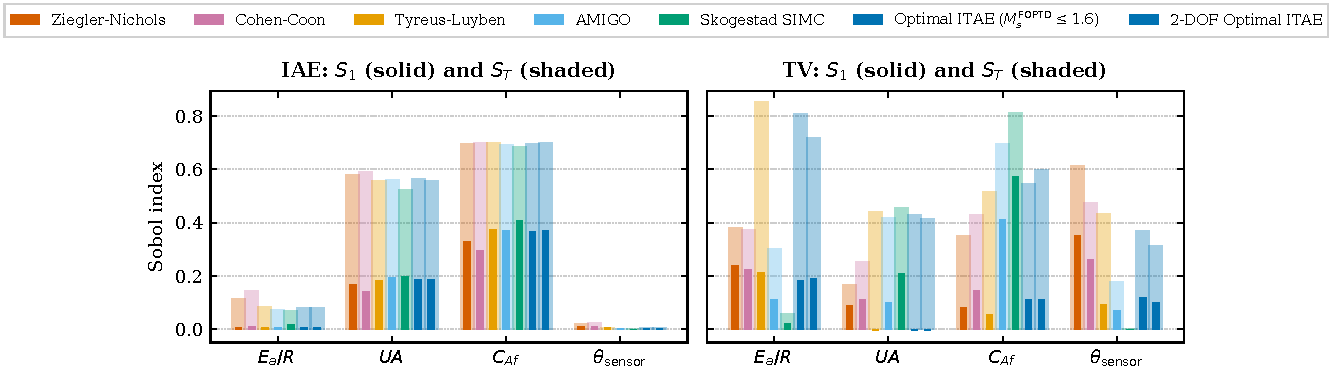
\includegraphics[width=0.92\textwidth]{figures/fig_sobol_indices.pdf}
    \caption{First-order ($S_1$, solid) and total-order ($S_T$, shaded) Sobol indices of IAE (left) and TV (right) for seven PID tunings.}
    \label{fig:sobol}
\end{figure*}

\begin{table*}[t]
\centering
\footnotesize
\caption{Global Sobol indices (Saltelli sampling, $N=512$, $3072$ closed-loop runs per controller) of IAE and TV for a $-2$~K setpoint step at $t = 0.5$~min under simultaneous uncertainty $E_a/R \in [0.97, 1.03]$, $UA \in [0.65, 1.05]\,UA_{\mathrm{nom}}$, $C_{Af} \in [0.85, 1.15]$~mol/L and sensor dead time $\theta_{\mathrm{sensor}} \in [0, 0.1]$~min. Every run starts from the nominal equilibrium. Entries are index $\pm$ half-width of the $95\%$ bootstrap interval (SALib, 100 resamples).}
\label{tab:sobol_sensitivity}
\resizebox{\ifdim\width>\textwidth\textwidth\else\width\fi}{!}{%
\begin{tabular}{lccccc}
\toprule
Controller & Parameter & $S_1$ (IAE) & $S_T$ (IAE) & $S_1$ (TV) & $S_T$ (TV) \\
\midrule
Ziegler-Nichols & $E_a/R$ & 0.006 $\pm$ 0.027 & 0.113 $\pm$ 0.032 & 0.234 $\pm$ 0.067 & 0.350 $\pm$ 0.061 \\
Ziegler-Nichols & $UA$ & 0.168 $\pm$ 0.097 & 0.559 $\pm$ 0.121 & 0.060 $\pm$ 0.054 & 0.193 $\pm$ 0.038 \\
Ziegler-Nichols & $C_{Af}$ & 0.354 $\pm$ 0.120 & 0.703 $\pm$ 0.165 & 0.111 $\pm$ 0.076 & 0.365 $\pm$ 0.053 \\
Ziegler-Nichols & $\theta_{\mathrm{sensor}}$ & 0.013 $\pm$ 0.012 & 0.017 $\pm$ 0.007 & 0.331 $\pm$ 0.073 & 0.519 $\pm$ 0.073 \\
Cohen-Coon & $E_a/R$ & 0.014 $\pm$ 0.032 & 0.138 $\pm$ 0.036 & 0.243 $\pm$ 0.075 & 0.389 $\pm$ 0.065 \\
Cohen-Coon & $UA$ & 0.148 $\pm$ 0.098 & 0.567 $\pm$ 0.122 & 0.098 $\pm$ 0.067 & 0.256 $\pm$ 0.045 \\
Cohen-Coon & $C_{Af}$ & 0.324 $\pm$ 0.118 & 0.707 $\pm$ 0.164 & 0.168 $\pm$ 0.082 & 0.424 $\pm$ 0.062 \\
Cohen-Coon & $\theta_{\mathrm{sensor}}$ & 0.016 $\pm$ 0.017 & 0.021 $\pm$ 0.007 & 0.215 $\pm$ 0.076 & 0.417 $\pm$ 0.065 \\
Tyreus-Luyben & $E_a/R$ & 0.009 $\pm$ 0.024 & 0.083 $\pm$ 0.023 & 0.292 $\pm$ 0.124 & 0.705 $\pm$ 0.180 \\
Tyreus-Luyben & $UA$ & 0.183 $\pm$ 0.093 & 0.523 $\pm$ 0.113 & 0.041 $\pm$ 0.100 & 0.475 $\pm$ 0.161 \\
Tyreus-Luyben & $C_{Af}$ & 0.414 $\pm$ 0.118 & 0.708 $\pm$ 0.162 & 0.041 $\pm$ 0.096 & 0.404 $\pm$ 0.117 \\
Tyreus-Luyben & $\theta_{\mathrm{sensor}}$ & 0.006 $\pm$ 0.008 & 0.007 $\pm$ 0.004 & 0.070 $\pm$ 0.047 & 0.320 $\pm$ 0.124 \\
AMIGO & $E_a/R$ & 0.008 $\pm$ 0.024 & 0.067 $\pm$ 0.018 & 0.174 $\pm$ 0.082 & 0.451 $\pm$ 0.138 \\
AMIGO & $UA$ & 0.198 $\pm$ 0.096 & 0.527 $\pm$ 0.115 & 0.081 $\pm$ 0.091 & 0.396 $\pm$ 0.100 \\
AMIGO & $C_{Af}$ & 0.410 $\pm$ 0.120 & 0.696 $\pm$ 0.163 & 0.334 $\pm$ 0.153 & 0.623 $\pm$ 0.108 \\
AMIGO & $\theta_{\mathrm{sensor}}$ & 0.003 $\pm$ 0.004 & 0.001 $\pm$ 0.000 & 0.111 $\pm$ 0.102 & 0.291 $\pm$ 0.135 \\
Skogestad SIMC & $E_a/R$ & 0.018 $\pm$ 0.025 & 0.063 $\pm$ 0.016 & 0.021 $\pm$ 0.027 & 0.057 $\pm$ 0.011 \\
Skogestad SIMC & $UA$ & 0.205 $\pm$ 0.086 & 0.485 $\pm$ 0.099 & 0.211 $\pm$ 0.077 & 0.449 $\pm$ 0.073 \\
Skogestad SIMC & $C_{Af}$ & 0.454 $\pm$ 0.115 & 0.695 $\pm$ 0.151 & 0.580 $\pm$ 0.093 & 0.813 $\pm$ 0.121 \\
Skogestad SIMC & $\theta_{\mathrm{sensor}}$ & 0.000 $\pm$ 0.001 & 0.000 $\pm$ 0.000 & 0.002 $\pm$ 0.002 & 0.001 $\pm$ 0.000 \\
Optimal ITAE ($M_s^{\mathrm{FOPTD}} \leq 1.6$) & $E_a/R$ & 0.008 $\pm$ 0.024 & 0.079 $\pm$ 0.022 & 0.243 $\pm$ 0.099 & 0.717 $\pm$ 0.195 \\
Optimal ITAE ($M_s^{\mathrm{FOPTD}} \leq 1.6$) & $UA$ & 0.189 $\pm$ 0.094 & 0.530 $\pm$ 0.115 & 0.021 $\pm$ 0.073 & 0.414 $\pm$ 0.134 \\
Optimal ITAE ($M_s^{\mathrm{FOPTD}} \leq 1.6$) & $C_{Af}$ & 0.407 $\pm$ 0.119 & 0.704 $\pm$ 0.163 & 0.081 $\pm$ 0.105 & 0.469 $\pm$ 0.126 \\
Optimal ITAE ($M_s^{\mathrm{FOPTD}} \leq 1.6$) & $\theta_{\mathrm{sensor}}$ & 0.005 $\pm$ 0.006 & 0.004 $\pm$ 0.003 & 0.093 $\pm$ 0.067 & 0.344 $\pm$ 0.136 \\
2-DOF Optimal ITAE & $E_a/R$ & 0.008 $\pm$ 0.024 & 0.083 $\pm$ 0.023 & 0.246 $\pm$ 0.110 & 0.634 $\pm$ 0.173 \\
2-DOF Optimal ITAE & $UA$ & 0.186 $\pm$ 0.093 & 0.525 $\pm$ 0.113 & 0.007 $\pm$ 0.087 & 0.415 $\pm$ 0.133 \\
2-DOF Optimal ITAE & $C_{Af}$ & 0.409 $\pm$ 0.119 & 0.707 $\pm$ 0.162 & 0.100 $\pm$ 0.103 & 0.554 $\pm$ 0.134 \\
2-DOF Optimal ITAE & $\theta_{\mathrm{sensor}}$ & 0.005 $\pm$ 0.007 & 0.005 $\pm$ 0.003 & 0.087 $\pm$ 0.057 & 0.257 $\pm$ 0.098 \\
\bottomrule
\end{tabular}%
}
\end{table*}


\begin{table*}[t]
\centering
\footnotesize
\caption{Uncertainty box of the Sobol analysis expressed as heat-removal demand: coolant flow needed at the $-2$~K setpoint when one factor sits at a bound and the others are nominal (nominal: $110.9$~L/min; valve stop $300$~L/min). Ranges of $E_a/R$ and $UA$ are relative to nominal.}
\label{tab:sobol_ranges}
\resizebox{\ifdim\width>\textwidth\textwidth\else\width\fi}{!}{%
\begin{tabular}{lccc}
\toprule
Factor & Range & \(u_{\mathrm{req}}\), low (L/min) & \(u_{\mathrm{req}}\), high (L/min) \\
\midrule
$E_a/R$ & [0.97, 1.03] & 124.0 & 90.8 \\
$UA$ & [0.65, 1.05] & 275.1 & 105.3 \\
$C_{Af}$ & [0.85, 1.15] & 60.3 & 208.1 \\
$\theta_{\mathrm{sensor}}$ & [0, 0.1] & -- & -- \\
\bottomrule
\end{tabular}%
}
\end{table*}


\paragraph{Reading with the intervals.} The intervals are wide ($\pm 0.11$ to $\pm 0.17$ on the total-order index of IAE for the two leading factors, up to $\pm 0.27$ for TV), and they restrict what can be read from the point estimates. For every tuning the variance of IAE is explained mainly by feed concentration ($S_T = 0.684$--$0.700$) and heat-transfer capacity ($S_T = 0.523$--$0.588$), whereas the activation energy ($S_T = 0.069$--$0.142$) and the sensor dead time ($S_T \le 0.025$) contribute little; the two leading factors are resolved from the two minor ones, but not from each other, and the seven tunings are not distinguishable in the IAE decomposition. Valve activity does tell them apart. For SIMC the variance of TV follows the physical load ($C_{Af}$: $S_T = 0.813 \pm 0.121$) and is insensitive to the sensor delay ($S_T = 0.001$), while for ZN the TV is dominated by $\theta_{\text{sensor}}$ ($S_1 = 0.351 \pm 0.089$, $S_T = 0.612 \pm 0.083$), and for TL, Optimal ITAE and 2-DOF Optimal ITAE by $E_a/R$ ($S_T = 0.851 \pm 0.266$, $0.807 \pm 0.249$, $0.719 \pm 0.222$), clearly above the $0.058 \pm 0.012$ of SIMC. The exact-loop margins of TL ($M_s^{\mathrm{lin}} = 1.15$, $\mathrm{PM} = 71^\circ$) and Optimal ITAE ($1.31$, $57^\circ$) do not mark them as low-margin loops, so low margin does not explain these differences; the cause is not identified. For every tuning $S_T$ substantially exceeds $S_1$ (e.g.\ TL, $UA$, TV: $S_1 = -0.006 \pm 0.066$, $S_T = 0.439 \pm 0.202$), and $\sum_i S_{Ti}$ of IAE reaches $1.46$ (CC): the uncertainties act jointly, so one-at-a-time robustness tests underestimate the effect of combined deviations.

\paragraph{Heat-removal demand and the feasible region.} In $11.4\%$ of the samples the setpoint requires $u_{\mathrm{req}} > 300$~L/min (Eq.~\eqref{eq:u_req}), so no controller can hold it, and these runs are expected to carry much of the variance of IAE. Only the \emph{first-order} indices could be recomputed on the feasible subset (Table~\ref{tab:sobol_feasible}, given-data RBD-FAST estimator): the Saltelli/Jansen estimators of the total-order index need the rectangular design of independent factors, which does not survive the removal of rows, and on the truncated box the factors are dependent, so the variance no longer decomposes additively and $S_T$ is not defined as before. The first-order index of $UA$ for IAE falls from $0.15$--$0.21$ over all samples to $0.03$--$0.07$ in the feasible region, and that of $C_{Af}$ from $0.29$--$0.41$ to $0.11$--$0.31$; the first-order indices of IAE add up to only $0.27$--$0.39$ there. A first-order index ignores interaction, so Table~\ref{tab:sobol_shapley} gives the Shapley effects, which divide the interaction among the factors and are defined for dependent inputs. Over $30$ seeds of the forest and of the cross-validation split, the mean effects for IAE give feed concentration $\vshapIAEcafmin$--$\vshapIAEcafmax$ and heat-transfer capacity $\vshapIAEuamin$--$\vshapIAEuamax$ of the explained variance, the activation energy $\vshapIAEeamin$--$\vshapIAEeamax$ and the sensor delay at most $\vshapIAEthmax$ (cross-validated $R^2$ of the four-factor model $\vshapIAErtwomin$--$\vshapIAErtwomax$). The half-widths of the $95\%$ intervals over seeds are at most $\vshaphwmax$: they show that the estimator is stable, not that the indices are known to that precision, since the Sobol sample itself was drawn once. Feed concentration and $UA$ therefore still lead in the feasible region, but $UA$ acts almost entirely through its interaction with the other factors. For TV the Shapley effects reproduce the picture of the total-order indices (ZN: sensor delay $\vshapTVZNth$; CC: delay $\vshapTVCCth$ and $E_a/R$ $\vshapTVCCea$; TL and the optimal tunings: $E_a/R$ $\vshapTVgroupeamin$--$\vshapTVgroupeamax$; SIMC: $C_{Af}$ $\vshapTVSIMCcaf$), with lower cross-validated $R^2$ ($\vshapTVrtwomin$--$\vshapTVrtwomax$). Table~\ref{tab:sobol_margin} tests the heat-removal-demand explanation directly. The Spearman correlation of IAE with $u_{\mathrm{req}}$ is positive for every tuning, but the share of rank variance it explains ($\rho_s^2$) is $0.18$ for CC and $0.33$ for ZN and $0.55$--$0.66$ for the other tunings, and it drops in the feasible region ($\rho_s = 0.20$ for CC to $0.74$ for SIMC). For TV the correlation is $+0.64$ for AMIGO and $+0.69$ for SIMC ($\rho_s^2 = 0.41$ and $0.48$), $+0.37$ to $+0.43$ for TL and the optimal tunings and negative for ZN and CC ($-0.18$ and $-0.37$), whose valve activity is bounded by the rate limit. The demand is therefore a partial, tuning-dependent explanation of both IAE and TV, not the whole account.

\begin{table*}[t]
\centering
\footnotesize
\caption{First-order indices from the given-data RBD-FAST estimator ($M = 10$) on all 3072 samples and on the 2721 samples with $u_{\mathrm{req}} \le u_{\max}$ (feasible region; $\pm$: half-width of the $95\%$ bootstrap interval). Total-order indices are not defined on the truncated region.}
\label{tab:sobol_feasible}
\resizebox{\ifdim\width>\textwidth\textwidth\else\width\fi}{!}{%
\begin{tabular}{lccccccccc}
\toprule
Method & Metric & $E_a/R$: all & $E_a/R$: feasible & $UA$: all & $UA$: feasible & $C_{Af}$: all & $C_{Af}$: feasible & $\theta_{\mathrm{sensor}}$: all & $\theta_{\mathrm{sensor}}$: feasible \\
\midrule
Ziegler-Nichols & IAE & 0.01 & 0.06 $\pm$ 0.05 & 0.18 & 0.04 $\pm$ 0.05 & 0.32 & 0.15 $\pm$ 0.04 & 0.00 & 0.02 $\pm$ 0.03 \\
Ziegler-Nichols & TV & 0.21 & 0.21 $\pm$ 0.04 & 0.03 & 0.01 $\pm$ 0.01 & 0.10 & 0.08 $\pm$ 0.03 & 0.33 & 0.38 $\pm$ 0.04 \\
Cohen-Coon & IAE & 0.01 & 0.11 $\pm$ 0.07 & 0.15 & 0.03 $\pm$ 0.04 & 0.29 & 0.11 $\pm$ 0.04 & 0.00 & 0.03 $\pm$ 0.03 \\
Cohen-Coon & TV & 0.22 & 0.23 $\pm$ 0.04 & 0.07 & 0.04 $\pm$ 0.02 & 0.15 & 0.12 $\pm$ 0.03 & 0.24 & 0.29 $\pm$ 0.04 \\
Tyreus-Luyben & IAE & 0.01 & 0.02 $\pm$ 0.02 & 0.20 & 0.05 $\pm$ 0.05 & 0.37 & 0.24 $\pm$ 0.03 & -0.00 & 0.00 $\pm$ 0.01 \\
Tyreus-Luyben & TV & 0.23 & 0.27 $\pm$ 0.04 & 0.00 & 0.02 $\pm$ 0.02 & 0.03 & 0.01 $\pm$ 0.03 & 0.04 & 0.05 $\pm$ 0.02 \\
AMIGO & IAE & 0.01 & 0.01 $\pm$ 0.02 & 0.21 & 0.07 $\pm$ 0.05 & 0.38 & 0.25 $\pm$ 0.03 & -0.00 & -0.00 $\pm$ 0.01 \\
AMIGO & TV & 0.09 & 0.16 $\pm$ 0.04 & 0.09 & 0.02 $\pm$ 0.02 & 0.36 & 0.24 $\pm$ 0.07 & 0.03 & 0.05 $\pm$ 0.03 \\
Skogestad SIMC & IAE & 0.02 & 0.01 $\pm$ 0.02 & 0.21 & 0.07 $\pm$ 0.05 & 0.41 & 0.31 $\pm$ 0.03 & -0.00 & -0.00 $\pm$ 0.01 \\
Skogestad SIMC & TV & 0.01 & 0.02 $\pm$ 0.02 & 0.18 & 0.04 $\pm$ 0.02 & 0.56 & 0.48 $\pm$ 0.04 & -0.00 & -0.00 $\pm$ 0.01 \\
Optimal ITAE ($M_s^{\mathrm{FOPTD}} \leq 1.6$) & IAE & 0.01 & 0.02 $\pm$ 0.02 & 0.20 & 0.06 $\pm$ 0.05 & 0.37 & 0.24 $\pm$ 0.03 & -0.00 & -0.00 $\pm$ 0.01 \\
Optimal ITAE ($M_s^{\mathrm{FOPTD}} \leq 1.6$) & TV & 0.19 & 0.24 $\pm$ 0.04 & 0.00 & 0.00 $\pm$ 0.01 & 0.06 & 0.03 $\pm$ 0.03 & 0.04 & 0.05 $\pm$ 0.03 \\
2-DOF Optimal ITAE & IAE & 0.01 & 0.02 $\pm$ 0.02 & 0.20 & 0.05 $\pm$ 0.05 & 0.37 & 0.24 $\pm$ 0.03 & -0.00 & -0.00 $\pm$ 0.01 \\
2-DOF Optimal ITAE & TV & 0.19 & 0.23 $\pm$ 0.03 & 0.00 & 0.01 $\pm$ 0.01 & 0.09 & 0.05 $\pm$ 0.03 & 0.04 & 0.05 $\pm$ 0.02 \\
\bottomrule
\end{tabular}%
}
\end{table*}


\begin{table*}[t]
\centering
\footnotesize
\caption{Shapley effects of the four uncertain factors on the feasible region ($u_{\mathrm{req}} \le u_{\max}$), where the truncated box makes the inputs dependent: shares of the explained variance (sum to one), from cross-validated random-forest conditional means; the last column is the cross-validated $R^2$ of the model with all four factors. Single run, no interval.}
\label{tab:sobol_shapley}
\resizebox{\ifdim\width>\textwidth\textwidth\else\width\fi}{!}{%
\begin{tabular}{lcccccc}
\toprule
Method & Metric & $E_a/R$ & $UA$ & $C_{Af}$ & $\theta_{\mathrm{sensor}}$ & \(R^2\) (all four) \\
\midrule
Ziegler-Nichols & IAE & 0.09 & 0.39 & 0.48 & 0.04 & 0.94 \\
Ziegler-Nichols & TV & 0.26 & 0.06 & 0.17 & 0.51 & 0.91 \\
Cohen-Coon & IAE & 0.16 & 0.36 & 0.43 & 0.04 & 0.93 \\
Cohen-Coon & TV & 0.30 & 0.11 & 0.20 & 0.38 & 0.90 \\
Tyreus-Luyben & IAE & 0.04 & 0.41 & 0.54 & 0.01 & 0.95 \\
Tyreus-Luyben & TV & 0.54 & 0.15 & 0.17 & 0.13 & 0.74 \\
AMIGO & IAE & 0.02 & 0.42 & 0.55 & 0.01 & 0.97 \\
AMIGO & TV & 0.25 & 0.18 & 0.45 & 0.11 & 0.83 \\
Skogestad SIMC & IAE & 0.03 & 0.38 & 0.59 & 0.01 & 0.95 \\
Skogestad SIMC & TV & 0.04 & 0.28 & 0.68 & 0.00 & 0.96 \\
Optimal ITAE ($M_s^{\mathrm{FOPTD}} \leq 1.6$) & IAE & 0.03 & 0.42 & 0.54 & 0.01 & 0.95 \\
Optimal ITAE ($M_s^{\mathrm{FOPTD}} \leq 1.6$) & TV & 0.50 & 0.16 & 0.21 & 0.13 & 0.70 \\
2-DOF Optimal ITAE & IAE & 0.04 & 0.41 & 0.54 & 0.01 & 0.96 \\
2-DOF Optimal ITAE & TV & 0.45 & 0.17 & 0.28 & 0.11 & 0.78 \\
\bottomrule
\end{tabular}%
}
\end{table*}


\begin{table*}[t]
\centering
\footnotesize
\caption{Spearman rank correlation, over the Sobol samples, between the closed-loop metrics and the steady coolant flow $u_{\mathrm{req}}$ that the perturbed plant needs at the new setpoint (heat-removal demand); last column: share of samples with $u_{\mathrm{req}}$ above the valve stop.}
\label{tab:sobol_margin}
\resizebox{\ifdim\width>\textwidth\textwidth\else\width\fi}{!}{%
\begin{tabular}{lccc}
\toprule
Method & \(\rho_s\)(IAE, \(u_{\mathrm{req}}\)) & \(\rho_s\)(TV, \(u_{\mathrm{req}}\)) & \(u_{\mathrm{req}} > u_{\max}\) (\%) \\
\midrule
Ziegler-Nichols & +0.57 & -0.35 & 11.4 \\
Cohen-Coon & +0.43 & -0.50 & 11.4 \\
Tyreus-Luyben & +0.73 & +0.29 & 11.4 \\
AMIGO & +0.79 & +0.61 & 11.4 \\
Skogestad SIMC & +0.81 & +0.70 & 11.4 \\
Optimal ITAE ($M_s^{\mathrm{FOPTD}} \leq 1.6$) & +0.74 & +0.36 & 11.4 \\
2-DOF Optimal ITAE & +0.73 & +0.34 & 11.4 \\
\bottomrule
\end{tabular}%
}
\end{table*}


\section{Second plant: heat exchanger}\label{supp:hx}
The second plant is built for this study as a reverse-acting, open-loop-stable process without reaction kinetics; it is not a published benchmark, and Seborg et al., Shinskey and Luyben only motivate its structure. A well-mixed shell (temperature $T_c$, coolant flow $q_c$, the manipulated input) cools a tube split into two cells in series ($T_1$, $T_2$); it is not a counter-current exchanger:
\begin{equation}
\begin{aligned}
\dot T_1 &= \tfrac{2q_p}{V_p}(T_{p,\mathrm{in}} - T_1) - \tfrac{UA(q_c)/2}{\rho_p C_{p,p} V_p/2}(T_1 - T_c), \\
\dot T_2 &= \tfrac{2q_p}{V_p}(T_1 - T_2) - \tfrac{UA(q_c)/2}{\rho_p C_{p,p} V_p/2}(T_2 - T_c), \\
\dot T_c &= \tfrac{q_c}{V_c}(T_{c,\mathrm{in}} - T_c) + \tfrac{UA(q_c)}{\rho_c C_{p,c} V_c}\bigl(\tfrac{T_1 + T_2}{2} - T_c\bigr),
\end{aligned}
\qquad UA(q_c) = UA_0\left(\frac{\max(q_c, 5)}{q_{c,ss}}\right)^{0.8},
\label{eq:hx}
\end{equation}
with output $y(t) = T_2(t - 0.20\text{ min})$ (a first-in first-out buffer of ten samples). Parameters: $V_p = 100$~L, $V_c = 40$~L, $q_p = 100$~L/min, $T_{p,\mathrm{in}} = 390$~K, $T_{c,\mathrm{in}} = 300$~K, $\rho C_p = 500$~cal/(L$\cdot$K) on both sides, $UA_0 = 6.0\times 10^4$~cal/(min$\cdot$K), $q_{c,ss} = u_{\text{bias}} = 100$~L/min; same valve, controller and $\Delta t$ as the reactor. The state is integrated by fixed-step fourth-order Runge--Kutta with four substeps per sample (\texttt{src/sim\_core/heat\_exchanger.py}). At $q_c = 100$~L/min, $T_{2,ss} = \vhxTss$~K and the eigenvalues lie between $\vhxeigfast$ and $\vhxeigslow$~min$^{-1}$; with the valve at its upper stop $T_2$ settles at $\vhxTinf$~K, below the setpoints of the steps, so the offset equilibrium of Proposition~\ref{prop:latch} exists. The transport delay was fixed before identification and not adjusted to reach a given $\theta/\tau$.

Table~\ref{tab:hx_gains} gives the identified model, the gains and $T_t^{\mathrm{cv}}$; Table~\ref{tab:hx_ablation} the seven policies on the three steps; Table~\ref{tab:hx_smax_map} the ratio $R$ against the slew limit. Sign-blind clamping never holds the valve at the upper stop on these steps (zero time at $u_{\max}$): ZN and CC oscillate through the slew limit without settling at a stop, which is why the latch does not appear, while their final errors in Table~\ref{tab:hx_ablation} reflect the phase of that oscillation at $t_f$. On the $\vhxncases$ cases of the full grid, $\rho \ge 1$ was followed by $R > 1$ in $\vhxnrhohihelp$ of $\vhxnrhohi$ (\texttt{results/jpc/hx\_rate\_demand\_grid.csv}); the exceptions are TL at every step and limit, with $R$ down to $\vhxbadRmin$, and one SIMC case.

\begin{table*}[t]
\centering
\footnotesize
\caption{Heat exchanger: FOPTD from a $+10$~L/min step ($K = -0.2036$~K/(L/min), $\tau = 0.657$~min, $\theta = 0.224$~min, $r = \theta/\tau = 0.341$, RMSE $0.0115$~K), the six loops tuned by the same rules (Optimal ITAE re-optimized on this plant under $M_s^{\mathrm{FOPTD}} \le 1.6$) and $T_t^{\mathrm{cv}}$ chosen by the criterion of Table~\ref{tab:antiwindup_tt_summary}.}
\label{tab:hx_gains}
\resizebox{\ifdim\width>\textwidth\textwidth\else\width\fi}{!}{%
\begin{tabular}{lccccc}
\toprule
Method & \(K_p\) ((L/min)/K) & \(T_i\) (min) & \(T_d\) (min) & \(M_s^{\mathrm{FOPTD}}\) & \(T_t^{\mathrm{cv}}\) (min) \\
\midrule
Ziegler-Nichols & -17.28 & 0.448 & 0.112 & 3.89 & 0.123 \\
Cohen-Coon & -20.43 & 0.485 & 0.077 & 4.28 & 0.166 \\
Tyreus-Luyben & -11.75 & 1.757 & 0.127 & 2.37 & 1.757 \\
AMIGO & -7.46 & 0.476 & 0.102 & 1.45 & 0.165 \\
Skogestad SIMC & -5.17 & 0.657 & 0.074 & 1.25 & 0.657 \\
Optimal ITAE ($M_s^{\mathrm{FOPTD}} \leq 1.6$) & -9.74 & 0.695 & 0.073 & 1.60 & 0.374 \\
\bottomrule
\end{tabular}%
}
\end{table*}


\begin{table*}[t]
\centering
\footnotesize
\caption{Heat exchanger: the seven integrator policies of Table~\ref{tab:antiwindup_ablation} (with back-calculation at both tracking constants) on $-2$, $-5$ and $+5$~K steps of the outlet temperature; IAE (K$\cdot$min) / overshoot (\%), final error and time at the upper stop of sign-blind clamping. Same valve ($[0, 300]$~L/min, $S_{\max} = 80$~L/min$^2$).}
\label{tab:hx_ablation}
\resizebox{\ifdim\width>\textwidth\textwidth\else\width\fi}{!}{%
\begin{tabular}{lccccccccccc}
\toprule
Step & Method & None & BC ($\sqrt{T_iT_d}$) & BC ($T_t^{\mathrm{cv}}$) & Sign-blind amp. & SB \(y(t_f) - y_{sp}\) (K) & SB at \(u_{\max}\) (min) & Amp. uncond. & Amp.+rate uncond. & Amp. direct. & Amp.+rate direct. (Eq.~\ref{eq:clamping_antiwindup}) \\
\midrule
$-2$ K & Ziegler-Nichols & 2.15 / 86.2 & 1.18 / 12.0 & 1.14 / 6.4 & 2.15 / 86.2 & -0.00 & 0.00 & 2.15 / 86.2 & 1.09 / 5.1 & 2.15 / 86.2 & 1.15 / 10.1 \\
 & Cohen-Coon & 4.73 / 110.8 & 1.07 / 8.9 & 1.06 / 4.8 & 4.73 / 110.8 & -0.00 & 0.00 & 4.73 / 110.8 & 1.16 / 13.2 & 4.73 / 110.8 & 1.09 / 13.2 \\
 & Tyreus-Luyben & 1.45 / 0.0 & 2.28 / 0.0 & 1.72 / 0.0 & 1.45 / 0.0 & +0.00 & 0.00 & 1.45 / 0.0 & 1.96 / 0.0 & 1.45 / 0.0 & 1.96 / 0.0 \\
 & AMIGO & 1.56 / 25.9 & 1.42 / 13.1 & 1.42 / 11.5 & 1.56 / 25.9 & +0.00 & 0.00 & 1.56 / 25.9 & 1.42 / 12.4 & 1.56 / 25.9 & 1.42 / 12.4 \\
 & Skogestad SIMC & 1.42 / 3.8 & 1.55 / 0.5 & 1.45 / 2.0 & 1.42 / 3.8 & -0.00 & 0.00 & 1.42 / 3.8 & 1.51 / 0.8 & 1.42 / 3.8 & 1.51 / 0.8 \\
 & Optimal ITAE ($M_s^{\mathrm{FOPTD}} \leq 1.6$) & 1.37 / 19.0 & 1.23 / 0.0 & 1.15 / 3.1 & 1.37 / 19.0 & -0.00 & 0.00 & 1.37 / 19.0 & 1.16 / 1.9 & 1.37 / 19.0 & 1.16 / 1.9 \\
$-5$ K & Ziegler-Nichols & 49.49 / 203.3 & 3.80 / 7.3 & 3.79 / 4.1 & 50.99 / 233.3 & -10.87 & 0.00 & 38.78 / 133.9 & 3.70 / 0.2 & 38.78 / 133.9 & 3.77 / 6.1 \\
 & Cohen-Coon & 54.98 / 182.1 & 3.62 / 0.9 & 3.68 / 0.0 & 60.58 / 186.1 & -3.17 & 0.00 & 37.96 / 129.7 & 3.97 / 6.2 & 37.96 / 129.7 & 3.69 / 6.2 \\
 & Tyreus-Luyben & 3.83 / 0.0 & 7.63 / 0.0 & 5.33 / 0.0 & 3.83 / 0.0 & +0.00 & 0.00 & 3.83 / 0.0 & 6.56 / 0.0 & 3.83 / 0.0 & 6.19 / 0.0 \\
 & AMIGO & 5.65 / 40.5 & 4.22 / 8.2 & 4.25 / 7.0 & 5.65 / 40.5 & +0.00 & 0.00 & 5.65 / 40.5 & 4.24 / 7.2 & 5.65 / 40.5 & 4.24 / 7.2 \\
 & Skogestad SIMC & 4.31 / 7.5 & 4.92 / 0.0 & 4.26 / 0.9 & 4.31 / 7.5 & -0.00 & 0.00 & 4.31 / 7.5 & 4.74 / 0.0 & 4.31 / 7.5 & 4.74 / 0.0 \\
 & Optimal ITAE ($M_s^{\mathrm{FOPTD}} \leq 1.6$) & 5.22 / 32.2 & 4.39 / 0.0 & 3.95 / 0.0 & 5.22 / 32.2 & -0.00 & 0.00 & 5.22 / 32.2 & 4.12 / 0.0 & 5.22 / 32.2 & 4.12 / 0.0 \\
$+5$ K & Ziegler-Nichols & 75.30 / 301.4 & 3.70 / 10.5 & 3.62 / 3.9 & 92.36 / 340.7 & -12.60 & 0.00 & 31.99 / 92.8 & 3.74 / 4.6 & 31.99 / 92.8 & 3.58 / 4.9 \\
 & Cohen-Coon & 80.32 / 318.2 & 3.55 / 7.3 & 3.52 / 2.3 & 95.90 / 371.6 & -18.22 & 0.00 & 33.03 / 87.1 & 4.36 / 18.7 & 33.03 / 87.1 & 3.86 / 18.7 \\
 & Tyreus-Luyben & 3.62 / 3.9 & 7.04 / 0.0 & 4.70 / 0.0 & 3.62 / 3.9 & +0.00 & 0.00 & 3.62 / 3.9 & 6.24 / 0.0 & 3.62 / 3.9 & 5.60 / 0.0 \\
 & AMIGO & 5.79 / 52.2 & 4.14 / 11.5 & 4.15 / 9.9 & 5.79 / 52.2 & +0.00 & 0.00 & 5.79 / 52.2 & 4.14 / 10.1 & 5.79 / 52.2 & 4.14 / 10.1 \\
 & Skogestad SIMC & 4.39 / 14.1 & 4.47 / 0.6 & 4.12 / 4.5 & 4.39 / 14.1 & -0.00 & 0.00 & 4.39 / 14.1 & 4.33 / 1.0 & 4.39 / 14.1 & 4.33 / 1.0 \\
 & Optimal ITAE ($M_s^{\mathrm{FOPTD}} \leq 1.6$) & 5.24 / 48.6 & 4.10 / 0.0 & 3.65 / 0.2 & 5.24 / 48.6 & +0.00 & 0.00 & 5.24 / 48.6 & 3.83 / 0.0 & 5.24 / 48.6 & 3.83 / 0.0 \\
\bottomrule
\end{tabular}%
}
\end{table*}


\begin{table*}[t]
\centering
\footnotesize
\caption{Heat exchanger: $R = \mathrm{IAE}_{\mathrm{amp}}/\mathrm{IAE}_{\mathrm{rate}}$ on the $-2$~K step against the slew limit (L/min$^2$), gains fixed; the full grid with the three steps and $\rho$ is in \texttt{results/jpc/hx\_rate\_demand\_grid.csv}.}
\label{tab:hx_smax_map}
\resizebox{\ifdim\width>\textwidth\textwidth\else\width\fi}{!}{%
\begin{tabular}{lccccccccc}
\toprule
Method & $S_{\max}=20$ & $S_{\max}=30$ & $S_{\max}=45$ & $S_{\max}=60$ & $S_{\max}=80$ & $S_{\max}=120$ & $S_{\max}=160$ & $S_{\max}=240$ & $S_{\max}=320$ \\
\midrule
Ziegler-Nichols & 11.43 & 14.29 & 12.78 & 2.80 & 1.87 & 1.48 & 1.37 & 1.25 & 1.17 \\
Cohen-Coon & 11.89 & 15.30 & 19.72 & 20.85 & 4.32 & 1.83 & 1.51 & 1.30 & 1.22 \\
Tyreus-Luyben & 0.71 & 0.60 & 0.65 & 0.70 & 0.74 & 0.80 & 0.84 & 0.90 & 0.92 \\
AMIGO & 1.64 & 1.38 & 1.24 & 1.16 & 1.10 & 1.05 & 1.03 & 1.02 & 1.01 \\
Skogestad SIMC & 1.03 & 0.95 & 0.93 & 0.94 & 0.94 & 0.96 & 0.97 & 0.98 & 0.99 \\
Optimal ITAE ($M_s^{\mathrm{FOPTD}} \leq 1.6$) & 1.42 & 1.32 & 1.27 & 1.21 & 1.18 & 1.12 & 1.09 & 1.06 & 1.04 \\
\bottomrule
\end{tabular}%
}
\end{table*}


\section{Short literature audit}\label{supp:audit}
To give a verifiable basis to any statement about how comparisons report their implementation, a short audit was run with a protocol registered before the search: OpenAlex, 2015--2026, three fixed search strings, inclusion of articles that compare control strategies on a CSTR or an equivalent chemical reactor with an actuator constraint in the methodology, candidates taken in the order of the database without regard to their results, and five items coded from the full text. Of $\vlitcandidates$ candidates, $\vlitcounted$ met the criteria and could be read in full; $\vlitabstract$ could be read only as abstracts, because the publisher blocked automated access, and are not counted. Table~\ref{tab:literature_audit} gives the counts; the full list with the reason for every exclusion is in \texttt{repository/literature\_audit.csv}. The sample is small, not systematic and coded by one reader, so it supports statements about these articles only.

\begin{table}[t]
\centering
\footnotesize
\setlength{\tabcolsep}{3pt}
\caption{Short literature audit (not a systematic review): what the articles that compare control strategies on a CSTR or equivalent reactor with an actuator constraint state about the implementation, counted over the articles read in full. Protocol, search strings and the list of every candidate are in \texttt{repository/literature\_audit.csv} and the repository report; anti-windup is not applicable to predictive controllers.}
\label{tab:literature_audit}
\begin{tabular}{lcccc}
\toprule
Item & yes & no & not applicable & not verifiable \\
\midrule
Actuator limits declared (amplitude) & 11 & 1 & 0 & 0 \\
Slew-rate limit declared & 0 & 12 & 0 & 0 \\
Backlash or deadband declared & 0 & 12 & 0 & 0 \\
Anti-windup logic declared & 2 & 5 & 5 & 0 \\
Loop action (reverse or direct) stated & 0 & 12 & 0 & 0 \\
Sampling interval and discretization method stated & 2 & 10 & 0 & 0 \\
Measurement noise or filter stated & 1 & 9 & 0 & 2 \\
\bottomrule
\end{tabular}
\end{table}


\bibliographystyle{elsarticle-num}
\bibliography{references}
\end{document}
